\documentclass[a4paper, 10pt, twoside]{report}

%%%%%%%%%%%%%%%%%%%%%%%%%%%%%%%%%%%%%%%%%%%%%%%%%%%%%%%%%%%%%%%%%%%%%%%%%
\usepackage[babel, titelside, en]{ku-forside} % KU-forside
\usepackage[a4paper]{geometry}  % Geometri-pakke: Styrer bl.a. maginer    %
\usepackage[round]{natbib}
\usepackage{blindtext}
\usepackage{mathpazo}
\usepackage{sectsty}
\usepackage{helvet}
\usepackage{pgfplots}
\usepackage{amsmath}
\usepackage{amsthm}
\usepackage{tikz}
\usetikzlibrary{arrows,shapes,positioning}
\usepackage[format=plain, labelfont={small, sf, bf}, textfont={small, sf, it}, singlelinecheck=off, margin={1cm, 0cm}, oneside, labelsep=newline]{caption}

% Change chapter headings to "Part"
\addto\captionsenglish{\renewcommand{\chaptername}{Part}}

% Change section headings to sans serif
\allsectionsfont{\normalfont\sffamily\bfseries}

% Enable definitions
\theoremstyle{definition}
\newtheorem{definition}{Definition}[section]
\newtheorem{theorem}{Theorem}[section]

% Math commands
\DeclareMathOperator*{\argmin}{arg\,min}
%
% Mini-manual til ku-forside pakken:
%
% Sprogmuligheder:     da, en
% babel loader babelpakken, med det valgte sprog
% Fakultetsmuligheder: farma, hum, jur, ku, life, nat, samf, sund, teo
% Farvemuligheder:     sh, farve
% Forsidemuligheder: lille, stor, titelside
%      titelside er identisk med designet p� ku.dk/designmanual
%      lille er giver et lille logo sammen med titlen p� den f�rste side
%      stor er giver et stort logo sammen med titlen p� den f�rste side
%
% Default er [da,nat,farve,titelside]
%
% Ex. \usepackage[babel, lille, jur, sh, en]{ku-forside} giver et lille logo i sorthvid for juridisk fakultet og loader babelpakken med engelsk som sprog.


\titel{Deep Multi-Task Learning} %
\undertitel{For Relation Extraction} %
\opgave{Master Thesis} % Findes kun under 'titelside'
\forfatter{Sune Andreas Dybro Debel}%
\dato{\today}%
\vejleder{Dirk Hovy} %  Findes kun under 'titelside'

\begin{document}
\maketitle
\thispagestyle{empty}
\newpage

\newgeometry{hmargin=4cm}
\begin{abstract}
\textit{In this thesis we investigate the usefulness of a multi-task, convolutional neural network architecture relation classification. We review the relevant theoretical and practical research literature for relation classification, supervised machine learning, convolutional neural networks, and deep multi-task learning. We test a state-of-the-art multi-task convolutional neural network architecture designed for relation classification on the SemEval 2010 Task 8 dataset. We investigate the sample complexity dynamics of learning this task simultaneously with other natural language processing tasks. We find that the architecture is ill-suited for this purpose. We discuss alternative approaches and make recommendations for further experimentation in this direction.}
\end{abstract}

\pagebreak
\newgeometry{twoside, inner=5cm, outer=3cm, vmargin=3cm}

\addtocontents{toc}{\protect\thispagestyle{empty}}

\tableofcontents
\setcounter{page}{0}
\chapter{Introduction}
\blindtext
\section{Information Extraction}
\label{information_extraction}
In natural language processing, information extraction is the problem of extracting structured information from unstructured text. Many practical information extraction problems fall in one of two categories: \textbf{named entity recognition} or \textbf{relation extraction} \citep{jurafsky09}. We introduce each of them in this section, and explain the challenges they pose.

\subsection{Named Entity Recognition}
\label{named_entity_recognition}
A named entity is roughly anything that has a proper name. The goal of named entity recognition (NER) is to label mentions of entities such as people, organizations or places occurring in natural language. The list of things these systems are tasked with recognizing is often extended to include things that aren't technically named entities such as amounts of money or calendar dates.

As an example, consider the sentence: 
$$
\text{Jim bought 300 shares of Acme Corp. in 2006.}
$$ 
A named entity recognition system designed to extract the entities \textit{person} and \textit{organization} should ideally assign the labels:
$$
	[\text{Jim}]_{person} \text{ bought 300 shares of } [\text{Acme Corp.}]_{organization} \text{ in 2006.}
$$
This is a difficult problem because of two types of ambiguity. Firstly, two distinct entities may share the same name and category, such as \textit{Francis Bacon} the painter and \textit{Francis Bacon} the philosopher. Secondly, two distinct entities can have the same name, but belong to different categories such as \textit{JFK} the former American president and \textit{JFK} the airport near New York. This means that named entity recognition systems need to have some model of the context in which these entities appear in order to produce correct output.
\\\\
Named entity recognition can be framed as a sequence labeling problem. A common approach is to apply so called tokenization to the text, i.e finding boundaries between words and punctuation, and associate each token with a label indicating which entity it belongs to. BIO-labeling (figure \ref{bio}) is a widely used labeling scheme in which token labels indicate whether the token is at the \textbf{B}eginning, \textbf{I}nside, or \textbf{O}utside an entity mention.
\begin{figure}
	\begin{center}
		\begin{tabular}{c c c c c c c c c c c}
	Jim & bought & 300 & shares & of & Acme & Corp & . & in & 2006 & . \\
	\texttt{B-PER} & \texttt{O} & \texttt{O} & \texttt{O} & \texttt{O} & \texttt{B-ORG} & \texttt{I-ORG} & \texttt{I-ORG} & \texttt{O} & \texttt{O} & \texttt{O}
	\end{tabular}
	\end{center}
	\caption{A sentence labeled with BIO labels for named entity recognition.}
	\label{bio}
\end{figure}

\subsection{Relation Extraction}
\label{relation_extract}
The goal of relation extraction is to identify relationships such as \textit{Family} or \textit{Employment} in natural language. The set of relations we would like a relation extraction system to recognize is commonly referred to as the \textbf{inventory}. Most often, the inventory is limited to relations between named entities. In some relation extraction tasks however, the goal is to more generally recognize relations between nominal expressions that include nouns and pronouns. \citep{hendrickx2009}. In both cases, the words between which a relation exists are referred to as the \textbf{arguments} of the relation.
\\\\
As an example, consider the sentence: 
$$
\text{Yesterday, New York based Foo Inc. announced their acquisition of Bar Corp.}
$$ 
Imagine we have designed a relation extraction system that recognizes the relation \textit{MergerBetween(organization, organization)} between two mentions of organizations. Ideally, we would like that system to extract the relation \textit{MergerBetween(Foo Inc., Bar Corp.)} from the above sentence.
\\\\
To simplify the relation extraction problem, it's often solved in three steps:
\begin{enumerate}
	\item \textbf{Named entity recognition} \enspace Identify the named entities in the input text.
	\item \textbf{Relation detection} \enspace For each pair of named entities in the input text, determine if a relation exists between them. This is a binary classification problem where the input is the text and the named entities detected in step 1, and the output is yes/no.
	\item \textbf{Relation classification} \enspace Classify each of the detected relations in the previous step. This a multi-label classification problem where the input is the input text and the named entities for which a relation was detected in step 2, and the output is a relation label.
\end{enumerate}
In this thesis we focus on step 3: assigning labels to detected relations. This is a difficult problem because of the high degree of ambiguity of natural language. As an example, consider the sentence 
\begin{quote}
	\textit{Susan left JFK.}
\end{quote}
Imagine that we want to design a relation extraction system that can detect the relations \textit{Physical(person, location): a person has a physical relation to a location} and \textit{Personal-Social(person, person): two persons have a social relation}. Both can reasonably be assigned the previous sentence, depending on whether \textit{JFK} refers to the airport near New York, or the former American president. Just as in named entity recognition, providing the correct label in this situation depends on context information.
\\\\
Early relation extraction systems relied on hand-crafted lexical and syntactic rules for detecting relations. \citet{hearst1992} is perhaps the earliest example of this approach. She considers the following sentence:
\begin{quote}
	\textit{Agar is a substance prepared from a mixture of red algae such as Gelidium for laboratory or industrial use.}
\end{quote}
Most people won't know what \textit{Gelidium} is. From the context we can infer that it's a type of algae however. She suggest that the following lexico-syntactic pattern between two noun phrases $NP_1$ and $NP_2$:
$$
NP_1\text{ such as }NP_2
$$
implies the relation $Hyponym(NP_1, NP_2)$. By performing a syntactic parse of the input sentence we can try to extract hyponym relations between noun phrases using such manually created rules. Because of the huge amount of variation found in natural languages, this is of course a cumbersome yet brittle approach.
\\\\
More recent solutions rely on supervised machine learning techniques to solve relation extraction problems. In this setting, a system learns to recognize relations in the inventory from annotated examples. The earliest examples of such systems relied on hand-crafted features of words in the neighborhood of the relation arguments, for example: \textit{the words separating the relation arguments are "such as"} \citep{jurafsky09}. As we will see in part \ref{neural_networks}, the promise of avoiding complicated hand-crafted features of the sentence, but having the system learn useful lexico-syntactic features on its own is the major attraction of solutions based on deep learning.

\subsection{Accuracy Measures}
Information extraction systems are often evaluated empirically by applying them to collections of text, so called corpora, in which $N$ mentions of named entities or relations are known. In these tests, accuracy measures for each class $c$ of information we wish to extract are usually defined in terms of how many times the system correctly predicted class $c$. Most metrics use the following terminology:

\begin{center}
	\begin{tabular}{r | c c}
	 & \textbf{predicted as $c$} & \textbf{predicted as not $c$}  \\ \hline
	$c$ & True positives ($tp$) & False negatives ($fn$) \\
	\textbf{not} $c$ & False positives ($fp$) & True negatives ($tn$)
\end{tabular}
\end{center}
Where for example $tp$ is the number of true positives produced for class $c$.
\\\\
The distribution of labels used in both named entity recognition and relation extraction is often highly imbalanced. Consider for example the BIO labelling scheme for named entity recognition in figure \ref{bio}. Most words will be outside a mention of a named entity, and will have the label \texttt{O}. Using simple accuracy $\frac{tp + tn}{tp + tn + fn + fp}$ as a performance metric for a system that outputs bio labels for each token in the text is therefore not very informative, since a useless system which labels all tokens with \texttt{O} would achieve high performance.
\\\\
\textbf{Precision} and \textbf{recall} are more appropriate performance metrics for this reason. Precision $\frac{tp}{tp + fp}$ is the fraction of information items for which the system predicted class $c$ that actually belonged to class $c$.
Recall $\frac{tp}{tp + fn}$ on the other hand is the fraction of information items in the corpora of class $c$ that the system correctly extracted.
\\\\
In a multi-class classification problem we are forced to decide how to average these metrics across classes. Specifically, there are two ways of averaging an accuracy measure across $C$ different classes: micro and macro averaging \citep{sokolova2009}. In macro averaging, an accuracy measure is computed for each class $c$ separately, and then averaged across all $C$ classes. For example macro-precision $p_{M}$:
$$
p_{M} = \frac{1}{C}\sum_{c=1}^C p_c
$$
Where $p_c$ is the precision of the system for class $c$. Micro averaging on the other hand, averages an accuracy by accumulating $tp$, $tn$, $fp$ and $fn$ across all $C$ classes. For example micro-precision $p_{\mu}$:
$$
p_\mu = \frac{\sum\limits_{c=1}^C tp_c}{\sum\limits_{c=1}^C tp_c + fp_c}
$$
Where for example $tp_c$ is the true positives a system produces for class $c$.
\\\\
The main difference between macro and micro averages of accuracy measures is that micro averaging gives more weight to more frequent classes. In other words, micro averaging encodes the bias that infrequent classes are unimportant, and a misclassification of an example of such a class should not penalize the accuracy measure as much as a misclassification of a more frequent class. Whether or not this a reasonable bias depends on the problem. In order to be agnostic about the frequency of semantic relations we use macro averaging for all our reporting in this thesis.
\\\\
To get a single number that summarizes the performance, precision $p$ and recall $r$ are often combined into a single metric: the $F1$ measure. $F1$ is defined as the harmonic mean of precision and recall $\frac{2pr}{p + r}$. Variations that use the micro and macro versions of precision and recall can naturally be computed as the harmonic mean of the micro or macro precision and recall respectively.

\chapter{Background}
\label{background}

In this part, we exemplify the information extraction problem and formally describe the supervised machine learning and multi-task learning setting. In addition, we describe neural networks, the concept of representation learning and its relevance to multi-task learning.

\section{Information Extraction}
\label{information_extraction}
In natural language processing, information extraction is the problem of extracting structured information from unstructured text. Many practical information extraction problems fall in one of two categories: \textbf{named entity recognition} or \textbf{relation extraction} \citep{jurafsky09}. We introduce each of them in this section, and explain the challenges they pose.

\subsection{Named Entity Recognition}
\label{named_entity_recognition}
A named entity is roughly anything that has a proper name. The goal of named entity recognition (NER) is to label mentions of entities such as people, organizations or places occurring in natural language. The list of things these systems are tasked with recognizing is often extended to include things that aren't technically named entities such as amounts of money or calendar dates.

As an example, consider the sentence: 
$$
\text{Jim bought 300 shares of Acme Corp. in 2006.}
$$ 
A named entity recognition system designed to extract the entities \textit{person} and \textit{organization} should ideally assign the labels:
$$
	[\text{Jim}]_{person} \text{ bought 300 shares of } [\text{Acme Corp.}]_{organization} \text{ in 2006.}
$$
This is a difficult problem because of two types of ambiguity. Firstly, two distinct entities may share the same name and category, such as \textit{Francis Bacon} the painter and \textit{Francis Bacon} the philosopher. Secondly, two distinct entities can have the same name, but belong to different categories such as \textit{JFK} the former American president and \textit{JFK} the airport near New York. This means that named entity recognition systems need to have some model of the context in which these entities appear in order to produce correct output.
\\\\
Named entity recognition can be framed as a sequence labeling problem. A common approach is to apply so called tokenization to the text, i.e finding boundaries between words and punctuation, and associate each token with a label indicating which entity it belongs to. BIO-labeling (figure \ref{bio}) is a widely used labeling scheme in which token labels indicate whether the token is at the \textbf{B}eginning, \textbf{I}nside, or \textbf{O}utside an entity mention.
\begin{figure}
	\begin{center}
		\begin{tabular}{c c c c c c c c c c c}
	Jim & bought & 300 & shares & of & Acme & Corp & . & in & 2006 & . \\
	\texttt{B-PER} & \texttt{O} & \texttt{O} & \texttt{O} & \texttt{O} & \texttt{B-ORG} & \texttt{I-ORG} & \texttt{I-ORG} & \texttt{O} & \texttt{O} & \texttt{O}
	\end{tabular}
	\end{center}
	\caption{A sentence labeled with BIO labels for named entity recognition.}
	\label{bio}
\end{figure}

\subsection{Relation Extraction}
\label{relation_extract}
The goal of relation extraction is to identify relationships such as \textit{Family} or \textit{Employment} in natural language. The set of relations we would like a relation extraction system to recognize is commonly referred to as the \textbf{inventory}. Most often, the inventory is limited to relations between named entities. In some relation extraction tasks however, the goal is to more generally recognize relations between nominal expressions that include nouns and pronouns. \citep{hendrickx2009}. In both cases, the words between which a relation exists are referred to as the \textbf{arguments} of the relation.
\\\\
As an example, consider the sentence: 
$$
\text{Yesterday, New York based Foo Inc. announced their acquisition of Bar Corp.}
$$ 
Imagine we have designed a relation extraction system that recognizes the relation \textit{MergerBetween(organization, organization)} between two mentions of organizations. Ideally, we would like that system to extract the relation \textit{MergerBetween(Foo Inc., Bar Corp.)} from the above sentence.
\\\\
To simplify the relation extraction problem, it's often solved in three steps:
\begin{enumerate}
	\item \textbf{Named entity recognition} \enspace Identify the named entities in the input text.
	\item \textbf{Relation detection} \enspace For each pair of named entities in the input text, determine if a relation exists between them. This is a binary classification problem where the input is the text and the named entities detected in step 1, and the output is yes/no.
	\item \textbf{Relation classification} \enspace Classify each of the detected relations in the previous step. This a multi-label classification problem where the input is the input text and the named entities for which a relation was detected in step 2, and the output is a relation label.
\end{enumerate}
In this thesis we focus on step 3: assigning labels to detected relations. This is a difficult problem because of the high degree of ambiguity of natural language. As an example, consider the sentence 
\begin{quote}
	\textit{Susan left JFK.}
\end{quote}
Imagine that we want to design a relation extraction system that can detect the relations \textit{Physical(person, location): a person has a physical relation to a location} and \textit{Personal-Social(person, person): two persons have a social relation}. Both can reasonably be assigned the previous sentence, depending on whether \textit{JFK} refers to the airport near New York, or the former American president. Just as in named entity recognition, providing the correct label in this situation depends on context information.
\\\\
Early relation extraction systems relied on hand-crafted lexical and syntactic rules for detecting relations. \citet{hearst1992} is perhaps the earliest example of this approach. She considers the following sentence:
\begin{quote}
	\textit{Agar is a substance prepared from a mixture of red algae such as Gelidium for laboratory or industrial use.}
\end{quote}
Most people won't know what \textit{Gelidium} is. From the context we can infer that it's a type of algae however. She suggest that the following lexico-syntactic pattern between two noun phrases $NP_1$ and $NP_2$:
$$
NP_1\text{ such as }NP_2
$$
implies the relation $Hyponym(NP_1, NP_2)$. By performing a syntactic parse of the input sentence we can try to extract hyponym relations between noun phrases using such manually created rules. Because of the huge amount of variation found in natural languages, this is of course a cumbersome yet brittle approach.
\\\\
More recent solutions rely on supervised machine learning techniques to solve relation extraction problems. In this setting, a system learns to recognize relations in the inventory from annotated examples. The earliest examples of such systems relied on hand-crafted features of words in the neighborhood of the relation arguments, for example: \textit{the words separating the relation arguments are "such as"} \citep{jurafsky09}. As we will see in part \ref{neural_networks}, the promise of avoiding complicated hand-crafted features of the sentence, but having the system learn useful lexico-syntactic features on its own is the major attraction of solutions based on deep learning.

\subsection{Accuracy Measures}
Information extraction systems are often evaluated empirically by applying them to collections of text, so called corpora, in which $N$ mentions of named entities or relations are known. In these tests, accuracy measures for each class $c$ of information we wish to extract are usually defined in terms of how many times the system correctly predicted class $c$. Most metrics use the following terminology:

\begin{center}
	\begin{tabular}{r | c c}
	 & \textbf{predicted as $c$} & \textbf{predicted as not $c$}  \\ \hline
	$c$ & True positives ($tp$) & False negatives ($fn$) \\
	\textbf{not} $c$ & False positives ($fp$) & True negatives ($tn$)
\end{tabular}
\end{center}
Where for example $tp$ is the number of true positives produced for class $c$.
\\\\
The distribution of labels used in both named entity recognition and relation extraction is often highly imbalanced. Consider for example the BIO labelling scheme for named entity recognition in figure \ref{bio}. Most words will be outside a mention of a named entity, and will have the label \texttt{O}. Using simple accuracy $\frac{tp + tn}{tp + tn + fn + fp}$ as a performance metric for a system that outputs bio labels for each token in the text is therefore not very informative, since a useless system which labels all tokens with \texttt{O} would achieve high performance.
\\\\
\textbf{Precision} and \textbf{recall} are more appropriate performance metrics for this reason. Precision $\frac{tp}{tp + fp}$ is the fraction of information items for which the system predicted class $c$ that actually belonged to class $c$.
Recall $\frac{tp}{tp + fn}$ on the other hand is the fraction of information items in the corpora of class $c$ that the system correctly extracted.
\\\\
In a multi-class classification problem we are forced to decide how to average these metrics across classes. Specifically, there are two ways of averaging an accuracy measure across $C$ different classes: micro and macro averaging \citep{sokolova2009}. In macro averaging, an accuracy measure is computed for each class $c$ separately, and then averaged across all $C$ classes. For example macro-precision $p_{M}$:
$$
p_{M} = \frac{1}{C}\sum_{c=1}^C p_c
$$
Where $p_c$ is the precision of the system for class $c$. Micro averaging on the other hand, averages an accuracy by accumulating $tp$, $tn$, $fp$ and $fn$ across all $C$ classes. For example micro-precision $p_{\mu}$:
$$
p_\mu = \frac{\sum\limits_{c=1}^C tp_c}{\sum\limits_{c=1}^C tp_c + fp_c}
$$
Where for example $tp_c$ is the true positives a system produces for class $c$.
\\\\
The main difference between macro and micro averages of accuracy measures is that micro averaging gives more weight to more frequent classes. In other words, micro averaging encodes the bias that infrequent classes are unimportant, and a misclassification of an example of such a class should not penalize the accuracy measure as much as a misclassification of a more frequent class. Whether or not this a reasonable bias depends on the problem. In order to be agnostic about the frequency of semantic relations we use macro averaging for all our reporting in this thesis.
\\\\
To get a single number that summarizes the performance, precision $p$ and recall $r$ are often combined into a single metric: the $F1$ measure. $F1$ is defined as the harmonic mean of precision and recall $\frac{2pr}{p + r}$. Variations that use the micro and macro versions of precision and recall can naturally be computed as the harmonic mean of the micro or macro precision and recall respectively.
\section{Supervised Machine Learning}
\label{supervised_machine_learning}

Most solutions to the information extraction problems in \ref{information_extraction} are based on supervised machine learning techniques. In this setting, a system learns to predict the named entities or relations between them given a unit of natural language by inspecting examples provided by a human annotator.

\subsection{The Supervised Learning Problem}
\label{the_supervised_learning_problem}
In general terms, a set $\mathcal{D}_{train}$ of $N$ training examples $(\mathbf{x}_i, \mathbf{y}_i)$ of inputs $\mathbf{x}_i$ and corresponding labels $\mathbf{y}_i$ is given, where each $\mathbf{x}_i$ belongs to a space $\mathcal{X}$ and each $\mathbf{y}_i$ belongs to a space $\mathcal{Y}$. At a later time, a new set of un-labeled inputs $\mathcal{D}_{test} = \{ \mathbf{x}_i \mid \mathbf{x}_i \in \mathcal{X}\}$ will be provided. The task is to learn a function $h: \mathcal{X} \mapsto \mathcal{Y}$ that performs well on $\mathcal{D}_{test}$. In particular, we are not explicitly interested in the performance of $h$ on $\mathcal{D}_{train}$ \citep{yaser12}.
\\\\
We can formalise the preference for functions $h$ that perform well on examples outside of the training set with a quantity known as \textbf{generalisation error}.

\begin{definition}[generalisation error]
	Let $P(\mathbf{x}, \mathbf{y})$ be a joint probability distribution over inputs $\mathbf{x} \in \mathcal{X}$ and labels $\mathbf{y} \in \mathcal{Y}$. Let $e(\mathbf{y}_1, \mathbf{y}_2)$ be an error measure that measures agreement between labels $\mathbf{y}_1$ and $\mathbf{y}_2$. Then the generalisation error $E$ of a function $h: \mathcal{X} \mapsto \mathcal{Y}$ is defined as:
	$$
		E(h) = \mathbb{E}_{\mathbf{x},\mathbf{y}\sim P(\mathbf{y}, \mathbf{x})}[e(h(\mathbf{x}), \mathbf{y})]
	$$
\end{definition}
Now, formally, the objective of supervised machine learning is to find a function $h^*$ that minimises $E(h)$ in a space of functions $\mathcal{H}$. Unfortunately, $P(\mathbf{x}, \mathbf{y})$ is unknown (if it was not, no learning would be required!). However, we can use $\mathcal{D}_{train}$ to estimate $E(h)$ with a quantity known as \textbf{training error}:

\begin{definition}[training error]
	Let $\mathcal{D}$ be a set of $N$ training examples $\{(\mathbf{x}_i, \mathbf{y}_i) \mid \mathbf{x}_i, \mathbf{y}_i \sim P(\mathbf{x}, \mathbf{y})\}$. Then the training error $\hat{E}$ is defined as:
	$$
		\hat{E}(h, \mathcal{D}) = \frac{1}{N}\sum\limits_{i=1}^N e(h(\mathbf{x}_i), \mathbf{y}_i)
	$$
\end{definition}
Using $\hat{E}$ to estimate $E$ is dangerous for two reasons. Firstly, $\mathcal{D}$ is a random quantity. It may happen that the samples available to us are not representative of $P(\mathbf{x}, \mathbf{y})$, leading us to choose $h$ that does not perform well in terms of $e$ on examples outside the training set.

Secondly, even if $\mathcal{D}$ is a good sample, it's possible to choose $h$ such that $\hat{E}$ is small, but $E$ is large. In particular, if $\mathcal{H}$ is very large, there likely exists a $h$ such that $\hat{E}(h, \mathcal{D}) = 0$. This is problematic for two reasons. Firstly the relationship between $\mathbf{x}$ and $\mathbf{y}$ may be noisy, that is $P(\mathbf{y} \mid \mathbf{x})$ is non-deterministic. In this case, by selecting $h$ such that $\hat{E}(h, \mathcal{D}) = 0$, we have fitted not only the general relationship between $\mathbf{x}$ and $\mathbf{y}$, but also the noise which is particular to $\mathcal{D}$.

Secondly, even if $P(\mathbf{y} \mid \mathbf{x})$ is deterministic, fitting it exactly will likely lead to poor generalisation since $\mathcal{D}$ is a finite sample. 
\\\\
Understanding the relationship between $E$, $\hat{E}$, $\mathcal{H}$ and $\mathcal{D}$ is the objective of a field of research known as \textbf{statistical learning theory}.

\subsection{Statistical Learning Theory}
In \ref{the_supervised_learning_problem} we argued informally that the relationship between $E$ and $\hat{E}$ depends on $\mathcal{D}$ and $\mathcal{H}$. The objective of statistical learning theory is to bound $E$ in terms of $\hat{E}$, $\mathcal{H}$ and $\mathcal{D}$. A central aspect of this problem is the question of what features of $\mathcal{H}$ determine how well $h^*$ fits $\mathcal{D}$, since the examples therein are finite and may be noisy.
\\\\
A \textbf{dichotomy} is an important concept in measuring how well $\mathcal{H}$ can fit an arbitrary $\mathcal{D}$.
\chapter{Neural Networks}
\label{neural_networks}

In this part we describe how to define $\mathcal{H}$ using functions called \textbf{neural networks}. These functions have the advantage of being easy to adapt to multi-task learning. We begin by describing how to design a $\mathcal{H}$ with neural networks. We then turn to the issue of how to use $\mathcal{D}$ to search this hypothesis space. Lastly, we introduce specialised neural networks that are useful for natural language processing.

\section{Feed-Forward Neural Networks}
\section{Learning Algorithm}
\label{learning_algorithm}
\subsection{Gradient Descent}
\subsection{Backpropagation}
\subsection{Regularisation}
\label{early_stopping}
\subsection{Adam}
\section{Convolutional Neural Networks}
A convolution $f * k$ is a mathematical operation that takes as input two functions $f$ and $k$.

\begin{definition}[convolution] \label{convolution}
	Let $f(x) \in \mathbb{R}$ and $k(x) \in \mathbb{R}$ be two real-valued functions defined for the entire real number line. Then the convolution $f * k$ is defined as
	$$
		(f * k)(x) = \int f(y)k(x - y)dy
	$$
\end{definition}

In practical applications involving computers, $f$ and $k$ are discrete, and the integral turns into a sum:
$$
(f * k)(x) = \sum\limits_{y=-\infty}^\infty f(y)k(x - y)
$$
Most functions in practical applications of convolutions represent signals such as images, sound or text, which are only defined over a limited range of indices $x$. In these cases, it's assumed that whenever $x$ is beyond the domain of $f$ or $k$ the output of either function is 0.
\\\\
We can think of a convolution as a weighted sum of the output of $f$ where the output of $k$ acts as the weights. This view of convolution is used heavily in signal processing applications where $k$ is chosen to produce certain properties in the convolution output such as reducing noise in $f$. In this setting $k$ is often referred to as a \textbf{kernel}. As an example, consider the noisy signal convolved with a gaussian kernel in figure \ref{gaussian_convolution}.

\begin{figure}
	\centering
	\input{img/gaussian.pgf}
	\caption{Visualisation of a noisy signal $f$ convolved with a small Gaussian kernel $k$. The output of the convolution $f * k$ captures the general trend of $f$ by averaging the outputs of $f$ at every $x$, such values of $f$ of inputs close to $x$ contribute more to the output of the convolution, than inputs far away from $x$ thanks to the weights of the Gaussian kernel.}
	\label{gaussian_convolution}
\end{figure}

\begin{figure}
	\centering
	\input{img/detector.pgf}
	\caption{Visualisation of convolutional kernel as feature detector. When the signal $f$ is similar to the kernel, the output of the convolution is maximally positive.}
	\label{feature_detector}
\end{figure}

The kernel $k$ can also act as a \textbf{feature detector}. When the output of $f$ is closely correlated with the output of $k$, the output of the convolution spikes. See for example figure \ref{feature_detector}.
\\\\
\textbf{Convolutional neural networks} are neural networks that take advantage of convolutions as feature detectors \citep{lecun1989}. By arranging the layers and weights in the network in specific ways, we can construct a network such that the output of each layer $l$ is the output of layer $l - 1$ convolved with a kernel $k$, where the weights of $k$ are exactly the neural network weights connecting the units in layer $l$ and $l - 1$.

Specifically, the weights connecting layers $l$ and $l - 1$ in a convolutional neural network should be arranged such that they are:

\begin{labeling}{shared}
	\item [\textbf{sparse}] each unit in layer $l$ receives input from a small number of units layer $l - 1$.
	\item [\textbf{shared}] the weights connecting units in layer $l$ and $l - 1$ are shared across the layer, in the same way that the same kernel weights are re-used around every index of $f$. See figure \ref{convolutional_network}.
\end{labeling}

These restrictions on the network architecture reduces the number of unique weights of the model. This improves the statistical efficiency of these types of models, i.e reduces the complexity of the induced hypothesis space \citep{goodfellow16}. Moreover, the reduction in the effective number of parameters has the effect of reducing both the memory requirements of storing the network, but also limits the number of operations required to compute the output of the network for a given input.
\\\\
Intuitively, the output at each unit $u$ in $l$ in a convolutional layer indicates how strongly the feature detected by the kernel given by its connecting weights is present in the output of units that $u$ connects to in layer $l - 1$. Since the weights are learned by gradient descent, the feature detected by units in layer $l$ is learnt as well.

Often, the simple presence or absence of a feature in the output of layer $l - 1$ is very informative for the classification task the convolutional network was built to solve. The exact position of a detected feature in layer $l - 1$ is often less informative however. For this reason, convolutional layers are often interleaved with so called \textbf{pooling layers}. The output of a pooling layer can be thought of as a summary how strongly a feature is detected in layer $l$, that discards information about the exact position at which the features was detected. Very commonly, max-pooling is used which simply outputs the maximum value over all outputs of units in layer $l$.

\begin{figure}[h]
	\centering
	\begin{tikzpicture}[->, >=stealth, swap]
			\node [neuron] (x1) at (0,0) {$x_1$};
			\node [neuron] (x2) at (1,0) {$x_2$};
			\node [neuron] (x3) at (2,0) {$x_3$};
			\node [neuron] (x4) at (3,0) {$x_4$};
			\node [neuron] (x5) at (4,0) {$x_5$};
			\node [neuron] (x6) at (5,0) {$x_6$};
			\node [neuron] (sigma1) at (1,2) {$\sigma$};
			\node [neuron] (sigma2) at (2,2) {$\sigma$};
			\node [neuron] (sigma3) at (3,2) {$\sigma$};
			\node [neuron] (sigma4) at (4,2) {$\sigma$};
			
			\draw (x1) edge[red] (sigma1);
			\draw (x2) edge[black] (sigma1);
			\draw (x3) edge[blue] (sigma1);
			
			\draw (x2) edge[red] (sigma2);
			\draw (x3) edge[black] (sigma2);
			\draw (x4) edge[blue] (sigma2);
			
			\draw (x3) edge[red] (sigma3);
			\draw (x4) edge[black] (sigma3);
			\draw (x5) edge[blue] (sigma3);
			
			\draw (x4) edge[red] (sigma4);
			\draw (x5) edge[black] (sigma4);
			\draw (x6) edge[blue] (sigma4);
	\end{tikzpicture}
	\caption{Visual representation of a one-dimensional convolution implemented as the first layer of a convolutional neural network. The connections between the input layer and the convolutional layer are sparse in that each unit is connected only to three of six inputs. The colors of the connections indicate how the weights are shared.}
	\label{convolutional_network}
\end{figure}



\section{Word Vectors}
The way text is represented in a computer doesn't in general encode any information about semantic similarities between words or sentences. Instead, text is most often represented as sequences of discrete symbols. Learning a $h$ that maps from discrete input space where distances between points don't encode similarity, such as words, to a prediction, such as the presence of a named entity, may be more difficult than learning a mapping from continuous input space to a prediction, since a continuous function can be expected to have some smoothness properties, i.e similar inputs should have similar outputs \citep{bengio2003}.
\\\\
For this reason some effort has been devoted to designing real-valued vector representation of words, so called \textbf{word vectors}, that encode semantic similarities such that words with similar meaning are close to each other in word-vector space. The notion of "meaning" of a word is a philosophically challenging one. A simple definition which leads to simple but useful algorithms is that words have similar meaning if they are used in similar contexts.

This leads to the idea of representing words as vectors of co-occurrence counts. Two words $w_i$ and $w_j$ co-occur in a context of $c$ words if $w_j$ appears somewhere in a window of $c$ words from $w_i$ in some piece of text. By representing $w_i$ as a vector $\vector{w}_i \in \mathbb{R}^V$ of co-occurrence counts for the $V$ words in some vocabulary, words that occur in similar contexts will be close to each other in co-occurrence vector space.
\\\\
The main problems with this representation is that $V$ may be very large, and $\vector{w}_i$ may be very sparse, that is, most of its components are 0 since most words never co-occur together. Recent solutions to this problem learn lower dimensional word vectors using co-occurrence statistics. \textbf{GloVe} is a recent and successful technique for learning word vectors that encode much useful syntactic and semantic information \citep{pennington2014}. In GloVe, each word $w_i$ is represented by a word vectors $\vector{w}_i$, and a context word vector $\tilde{\vector{w}}_i$. The vectors are initialized randomly

 Glove vectors are learned by minimizing the objective function:
$$
\sum\limits_{i=1}^V\sum\limits_{i=1}^V f(\matrix{X}_{ij})(\vector{w}_i^T\tilde{\vector{w}}_j + b_i + \tilde{b}_j - \ln \matrix{X}_{ij})^2
$$
Where $\matrix{X}_{ij}$ is the co-occurrence count for word $w_i$ and $w_j$, and $b_i$ and $\tilde{b}_j$ are bias terms. $f$ is a weighting function that gives low weight to infrequent terms and caps extremely frequent terms, defined as:
$$
f(x) = \begin{cases}
	(x / x_{max})^{3/4} & \text{when $x < x_{max}$} \\
	1 & \text{otherwise}
\end{cases}
$$
Minimizing this objective leads to word vectors whose dot products are close to log-co-occurrence counts for the words they represent. It can be shown that this has the effect that word vector differences encode information about ratios of log-co-occurrence probabilities which are highly informative of semantic similarity.
\\\\
It is now common practice to incorporate word vectors in neural network models for natural language processing tasks in a so called embedding layer. In this scheme, the components of the word vectors are parameters that can be trained by back propagation to yield word vector representations that are informative for a given task. These word embedding vectors, or simply word embeddings, can be initialized with small random components as any other neural network parameter, or they can be initialized with pre-learned word vectors, for example GloVe vectors.
\chapter{Multi-Task Learning}
\label{multi-task_learning}
\section{Representation Learning}
\label{representation_learning}
\section{Deep Multi-Task Learning}
\label{deep_multi-task_learning}
Neural networks have the advantage of being easy to adapt from single-task learning to multi-task learning. The simplest way of turning two single task learning problems into a multi-task learning problem using neural networks is by hard weight sharing of a subset of the weights of the networks for the learning tasks and learning them simultaneously \citep{caruana1997}. As an example, consider figure \ref{no_weight_sharing} and \ref{weight_sharing}.
\\\\
\begin{figure}[h]
	\centering
	\begin{tikzpicture}[->, >=stealth, swap]
			\node [neuron] (x11) at (0,0) {};
			\node [neuron] (x12) at (1,0) {};
			\node [neuron] (x13) at (2,0) {};
			\node [neuron] (x14) at (3,0) {};
			\node [neuron] (x15) at (4,0) {};
			\node [neuron] (sigma11) at (1,1.5) {};
			\node [neuron] (sigma12) at (2,1.5) {};
			\node [neuron] (sigma13) at (3,1.5) {};
			\node [neuron] (out1) at (2,3) {};	
			\node [] (label1) at (2,4) {Task 1};	
			\draw (x11) edge (sigma11);
			\draw (x12) edge (sigma11);
			\draw (x13) edge (sigma11);
			
			\draw (x12) edge (sigma12);
			\draw (x13) edge (sigma12);
			\draw (x14) edge (sigma12);
			
			\draw (x13) edge (sigma13);
			\draw (x14) edge (sigma13);
			\draw (x15) edge (sigma13);
			
			\draw (sigma11) edge (out1);
			\draw (sigma12) edge (out1);
			\draw (sigma13) edge (out1);
			
			\node [neuron] (x21) at (6,0) {};
			\node [neuron] (x22) at (7,0) {};
			\node [neuron] (x23) at (8,0) {};
			\node [neuron] (x24) at (9,0) {};
			\node [neuron] (x25) at (10,0) {};
			\node [neuron] (sigma21) at (7,1.5) {};
			\node [neuron] (sigma22) at (8,1.5) {};
			\node [neuron] (sigma23) at (9,1.5) {};
			\node [neuron] (out2) at (8,3) {};	
			\node [] (label2) at (8,4) {Task 2};	
			\draw (x21) edge (sigma21);
			\draw (x22) edge (sigma21);
			\draw (x23) edge (sigma21);
			
			\draw (x22) edge (sigma22);
			\draw (x23) edge (sigma22);
			\draw (x24) edge (sigma22);
			
			\draw (x23) edge (sigma23);
			\draw (x24) edge (sigma23);
			\draw (x25) edge (sigma23);
			
			\draw (sigma21) edge (out2);
			\draw (sigma22) edge (out2);
			\draw (sigma23) edge (out2);
	\end{tikzpicture}
	\caption{Visual representation of single-task learning with neural networks. A set of neural network weights are learnt separately for Task 1 and Task 2.}
	\label{no_weight_sharing}
\end{figure}

\begin{figure}[h]
	\centering
	\begin{tikzpicture}[->, >=stealth, swap]
			\node [neuron] (x1) at (0,0) {};
			\node [neuron] (x2) at (1,0) {};
			\node [neuron] (x3) at (2,0) {};
			\node [neuron] (x4) at (3,0) {};
			\node [neuron] (x5) at (4,0) {};
			\node [neuron] (sigma1) at (1,1.5) {};
			\node [neuron] (sigma2) at (2,1.5) {};
			\node [neuron] (sigma3) at (3,1.5) {};
			\node [neuron] (out1) at (1.3,3) {};	
			\node [neuron] (out2) at (2.7,3) {};
			\node [] (label1) at (1.3,4) {Task 1};
			\node [] (label2) at (2.7,4) {Task 2};
			\draw (x1) edge (sigma1);
			\draw (x2) edge (sigma1);
			\draw (x3) edge (sigma1);
			
			\draw (x2) edge (sigma2);
			\draw (x3) edge (sigma2);
			\draw (x4) edge (sigma2);
			
			\draw (x3) edge (sigma3);
			\draw (x4) edge (sigma3);
			\draw (x5) edge (sigma3);
			
			\draw (sigma1) edge (out1);
			\draw (sigma2) edge (out1);
			\draw (sigma3) edge (out1);
			
			\draw (sigma1) edge (out2);
			\draw (sigma2) edge (out2);
			\draw (sigma3) edge (out2);
	\end{tikzpicture}
	\caption{Visual representation multi-task learning with neural networks. The weights of the hidden layer is shared between the two tasks.}
	\label{weight_sharing}
\end{figure}
\noindent
Multi-task learning techniques that are based on sharing neural network weights between tasks are collectively known as \textbf{deep multi-task learning} techniques. Deep multi-task learning is closely associated with the idea of representation learning presented in section \ref{representation_learning} and the more general framework of bias learning presented in section \ref{bias_learning}. The network represents a shared representation $f(\vector{x})$ represented by $S$ shared layers, often the first layers, and hypotheses $h_1 = (g_1 \circ f)(\vector{x})$ to $h_M = (g_M \circ f)(\vector{x})$ for each learning task, where $g_m$ is $L - S$ neural network layers specific to each task.
\\\\
The exact circumstances under which deep multi-task learning leads to lower overall generalization error compared to deep single-task learning are not yet theoretically well understood. \citet{caruana1997} lists 3 suggestions for how multi-task learning can reduce generalization error:
\begin{description}
	\item [Statistical Data Amplification] The effective number of training examples available to a deep multi-task learning system is increased due to the examples in the auxiliary data. The extensions to the Vapnik-Chervonenkis bound seen in the preceding sections gives us confidence that this reduces the risk that generalization error is far away from training error.
	\item [Eavesdropping] If a hidden layer feature is useful to both Task 1 and Task 2, but much easier to learn when learning Task 2, sharing the hidden layer between the two tasks is likely to reduce generalization error for Task 1.
	\item [Representation Bias] If Task 1 and Task 2 share a common minimum in weight-space, learning the tasks with weight sharing biases the learning system to choose the shared minimum. This is effectively a form of regularization that forces the learning system to search for a good hypothesis in a hypothesis space that is restricted to hypotheses that are useful for more than one task.
\end{description}
\noindent
\citet{baxter2000} applies his bias learning framework to the case where the hypothesis space family $\mathbb{H}$ is constructed of neural networks where the first two layers are shared between tasks.

Specifically, a feature map $\phi_{\vector{w}}:\mathbb{R}^d\mapsto\mathbb{R}^{d^{(2)}}$ is a two layer neural network parameterized by $\vector{w}$ that maps an input vector $\vector{x} \in \mathbb{R}^d$ to feature vector $\phi_{\vector{w}}(\vector{x})$. Each feature $\phi_{\vector{w},j} \in \phi_{\vector{w}}$ is defined by:
$$
\phi_{\vector{w},j}(\vector{x}) = \sigma\left( w_{0j} + \sum\limits_{i=1}^{d^{(1)}} w_{ij}h_i(\vector{x}) \right)
$$
\noindent
$h_{i}$ is the output of unit $i$ in the first layer, $w_{ij}$ is the weight connecting unit $\phi_{\vector{w},j}$ and $i$ and $w_{0j}$ is the bias weight. For simplicity, \citet{baxter2000} considers only the binary threshold activation function:
$$
\sigma(a) = \begin{cases}
	+1 & \text{when } a \geq 0 \\
	-1 & \text{otherwise}
\end{cases}
$$
The output of each unit in the first layer $h_j$ is computed as
$$
h_j(\vector{x}) = \sigma\left( v_{0j} + \sum\limits_{i=1}^{d} v_{ij}x_{i} \right)
$$

where $v_{ij}$ is the weight connecting the input feature $x_i$ to unit $j$ in the first layer and $v_{0j}$ is a bias weight. The total number of weights $W$ in these two layers is thus $W = d^{(1)}(d^{(0)} + 1) + d^{(0)}(d + 1)$. The space of all such feature maps $\{\phi_{\vector{w}} \mid \vector{w} \in \mathbb{R}^W\}$ can be thought of as the representation space $\mathcal{F}$ in the representation learning framework of \citet{baxter1995}.
\\\\
\cite{baxter2000} defines a hypothesis space $\hypspace_{\vector{w}}$ as a set of binary decision functions on top the feature maps. Specifically:
$$
\hypspace_{\vector{w}} = \left\{ \sigma\left(  a_{0} + \sum\limits_{i=1}^{d^{(2)}} a_i\phi_{\vector{w},i}\right) \;\middle| \; a_{0},\dots,a_{d^{(2)}} \in \mathbb{R} \right\}
$$
where $a_i$ is the weight connecting feature $\phi_{\vector{w},i}$ and the output unit and $a_0$ is a bias weight. The set of all such hypothesis spaces can be considered a hypothesis space $\mathbb{H}$ family such that:
$$
\mathbb{H} = \{\hypspace_{\vector{w}} \mid \vector{w} \in \mathbb{R}^W\}
$$
Recall that the goal in bias learning is to select a vector $\vector{h}$ of M hypotheses $h_m$ that minimizes the average generalization error $E(\vector{h}) = \frac{1}{M}\sum_{m=1}^M E_m(h_m)$. With the limitations described above, \citet{baxter2000} is able to show that in order for the average empirical error $\hat{E}(\vector{h}, \data_M)$ to be within $\epsilon$ of the average generalization error $E(\vector{h})$ with probability $1 - \delta$, it suffices that the number of examples $N$ per task satisfies:
$$
N \geq O\left( \frac{1}{\epsilon^2}\left( \frac{W}{M} + d^{(2)} + 1\right)\log \frac{1}{\epsilon} + \frac{1}{M}\log\frac{1}{\delta} \right)
$$
Ignoring the confidence parameters $\epsilon$ and $\delta$, the sample complexity bound tells us that learning complicated neural network representations where $d^{(1)}$ and $d^{(2)}$ and therefore also $W$ are large, is harder than learning simple representations in the sense that it requires more samples to succeed. The benefit gained by multi-task learning is that we can reduce $N$ by increasing $M$, an option we don't have in the single task learning setting. This means we can afford to learn more complicated representations in the hope that this can lead to lower training error for one or more tasks and still have high confidence that generalization is possible by increasing $M$.
\section{Summary}

\chapter{Neural Networks}
\label{neural_networks}

In this part we describe how to define $\mathcal{H}$ using functions called \textbf{neural networks}. These functions have the advantage of being easy to adapt to multi-task learning. We begin by describing how to design a $\mathcal{H}$ with neural networks. We then turn to the issue of how to use $\mathcal{D}$ to search this hypothesis space. Lastly, we introduce specialised neural networks that are useful for natural language processing.

\section{Feed-Forward Neural Networks}
\section{Learning Algorithm}
\label{learning_algorithm}
\subsection{Gradient Descent}
\subsection{Backpropagation}
\subsection{Regularisation}
\label{early_stopping}
\subsection{Adam}
\section{Convolutional Neural Networks}
A convolution $f * k$ is a mathematical operation that takes as input two functions $f$ and $k$.

\begin{definition}[convolution] \label{convolution}
	Let $f(x) \in \mathbb{R}$ and $k(x) \in \mathbb{R}$ be two real-valued functions defined for the entire real number line. Then the convolution $f * k$ is defined as
	$$
		(f * k)(x) = \int f(y)k(x - y)dy
	$$
\end{definition}

In practical applications involving computers, $f$ and $k$ are discrete, and the integral turns into a sum:
$$
(f * k)(x) = \sum\limits_{y=-\infty}^\infty f(y)k(x - y)
$$
Most functions in practical applications of convolutions represent signals such as images, sound or text, which are only defined over a limited range of indices $x$. In these cases, it's assumed that whenever $x$ is beyond the domain of $f$ or $k$ the output of either function is 0.
\\\\
We can think of a convolution as a weighted sum of the output of $f$ where the output of $k$ acts as the weights. This view of convolution is used heavily in signal processing applications where $k$ is chosen to produce certain properties in the convolution output such as reducing noise in $f$. In this setting $k$ is often referred to as a \textbf{kernel}. As an example, consider the noisy signal convolved with a gaussian kernel in figure \ref{gaussian_convolution}.

\begin{figure}
	\centering
	%% Creator: Matplotlib, PGF backend
%%
%% To include the figure in your LaTeX document, write
%%   \input{<filename>.pgf}
%%
%% Make sure the required packages are loaded in your preamble
%%   \usepackage{pgf}
%%
%% Figures using additional raster images can only be included by \input if
%% they are in the same directory as the main LaTeX file. For loading figures
%% from other directories you can use the `import` package
%%   \usepackage{import}
%% and then include the figures with
%%   \import{<path to file>}{<filename>.pgf}
%%
%% Matplotlib used the following preamble
%%   \usepackage{fontspec}
%%   \setmainfont{Palatino}
%%   \setsansfont{Lucida Grande}
%%   \setmonofont{Andale Mono}
%%
\begingroup%
\makeatletter%
\begin{pgfpicture}%
\pgfpathrectangle{\pgfpointorigin}{\pgfqpoint{4.940612in}{2.730000in}}%
\pgfusepath{use as bounding box, clip}%
\begin{pgfscope}%
\pgfsetbuttcap%
\pgfsetmiterjoin%
\definecolor{currentfill}{rgb}{1.000000,1.000000,1.000000}%
\pgfsetfillcolor{currentfill}%
\pgfsetlinewidth{0.000000pt}%
\definecolor{currentstroke}{rgb}{1.000000,1.000000,1.000000}%
\pgfsetstrokecolor{currentstroke}%
\pgfsetdash{}{0pt}%
\pgfpathmoveto{\pgfqpoint{0.000000in}{0.000000in}}%
\pgfpathlineto{\pgfqpoint{4.940612in}{0.000000in}}%
\pgfpathlineto{\pgfqpoint{4.940612in}{2.730000in}}%
\pgfpathlineto{\pgfqpoint{0.000000in}{2.730000in}}%
\pgfpathclose%
\pgfusepath{fill}%
\end{pgfscope}%
\begin{pgfscope}%
\pgfsetbuttcap%
\pgfsetmiterjoin%
\definecolor{currentfill}{rgb}{1.000000,1.000000,1.000000}%
\pgfsetfillcolor{currentfill}%
\pgfsetlinewidth{0.000000pt}%
\definecolor{currentstroke}{rgb}{0.000000,0.000000,0.000000}%
\pgfsetstrokecolor{currentstroke}%
\pgfsetstrokeopacity{0.000000}%
\pgfsetdash{}{0pt}%
\pgfpathmoveto{\pgfqpoint{0.273112in}{0.017500in}}%
\pgfpathlineto{\pgfqpoint{4.923112in}{0.017500in}}%
\pgfpathlineto{\pgfqpoint{4.923112in}{2.712500in}}%
\pgfpathlineto{\pgfqpoint{0.273112in}{2.712500in}}%
\pgfpathclose%
\pgfusepath{fill}%
\end{pgfscope}%
\begin{pgfscope}%
\pgfsetbuttcap%
\pgfsetroundjoin%
\definecolor{currentfill}{rgb}{0.000000,0.000000,0.000000}%
\pgfsetfillcolor{currentfill}%
\pgfsetlinewidth{0.803000pt}%
\definecolor{currentstroke}{rgb}{0.000000,0.000000,0.000000}%
\pgfsetstrokecolor{currentstroke}%
\pgfsetdash{}{0pt}%
\pgfsys@defobject{currentmarker}{\pgfqpoint{0.000000in}{-0.048611in}}{\pgfqpoint{0.000000in}{0.000000in}}{%
\pgfpathmoveto{\pgfqpoint{0.000000in}{0.000000in}}%
\pgfpathlineto{\pgfqpoint{0.000000in}{-0.048611in}}%
\pgfusepath{stroke,fill}%
}%
\begin{pgfscope}%
\pgfsys@transformshift{0.484476in}{1.339482in}%
\pgfsys@useobject{currentmarker}{}%
\end{pgfscope}%
\end{pgfscope}%
\begin{pgfscope}%
\pgftext[x=0.484476in,y=1.242260in,,top]{\rmfamily\fontsize{8.000000}{9.600000}\selectfont 0}%
\end{pgfscope}%
\begin{pgfscope}%
\pgfsetbuttcap%
\pgfsetroundjoin%
\definecolor{currentfill}{rgb}{0.000000,0.000000,0.000000}%
\pgfsetfillcolor{currentfill}%
\pgfsetlinewidth{0.803000pt}%
\definecolor{currentstroke}{rgb}{0.000000,0.000000,0.000000}%
\pgfsetstrokecolor{currentstroke}%
\pgfsetdash{}{0pt}%
\pgfsys@defobject{currentmarker}{\pgfqpoint{0.000000in}{-0.048611in}}{\pgfqpoint{0.000000in}{0.000000in}}{%
\pgfpathmoveto{\pgfqpoint{0.000000in}{0.000000in}}%
\pgfpathlineto{\pgfqpoint{0.000000in}{-0.048611in}}%
\pgfusepath{stroke,fill}%
}%
\begin{pgfscope}%
\pgfsys@transformshift{1.495785in}{1.339482in}%
\pgfsys@useobject{currentmarker}{}%
\end{pgfscope}%
\end{pgfscope}%
\begin{pgfscope}%
\pgftext[x=1.495785in,y=1.242260in,,top]{\rmfamily\fontsize{8.000000}{9.600000}\selectfont 5}%
\end{pgfscope}%
\begin{pgfscope}%
\pgfsetbuttcap%
\pgfsetroundjoin%
\definecolor{currentfill}{rgb}{0.000000,0.000000,0.000000}%
\pgfsetfillcolor{currentfill}%
\pgfsetlinewidth{0.803000pt}%
\definecolor{currentstroke}{rgb}{0.000000,0.000000,0.000000}%
\pgfsetstrokecolor{currentstroke}%
\pgfsetdash{}{0pt}%
\pgfsys@defobject{currentmarker}{\pgfqpoint{0.000000in}{-0.048611in}}{\pgfqpoint{0.000000in}{0.000000in}}{%
\pgfpathmoveto{\pgfqpoint{0.000000in}{0.000000in}}%
\pgfpathlineto{\pgfqpoint{0.000000in}{-0.048611in}}%
\pgfusepath{stroke,fill}%
}%
\begin{pgfscope}%
\pgfsys@transformshift{2.507094in}{1.339482in}%
\pgfsys@useobject{currentmarker}{}%
\end{pgfscope}%
\end{pgfscope}%
\begin{pgfscope}%
\pgftext[x=2.507094in,y=1.242260in,,top]{\rmfamily\fontsize{8.000000}{9.600000}\selectfont 10}%
\end{pgfscope}%
\begin{pgfscope}%
\pgfsetbuttcap%
\pgfsetroundjoin%
\definecolor{currentfill}{rgb}{0.000000,0.000000,0.000000}%
\pgfsetfillcolor{currentfill}%
\pgfsetlinewidth{0.803000pt}%
\definecolor{currentstroke}{rgb}{0.000000,0.000000,0.000000}%
\pgfsetstrokecolor{currentstroke}%
\pgfsetdash{}{0pt}%
\pgfsys@defobject{currentmarker}{\pgfqpoint{0.000000in}{-0.048611in}}{\pgfqpoint{0.000000in}{0.000000in}}{%
\pgfpathmoveto{\pgfqpoint{0.000000in}{0.000000in}}%
\pgfpathlineto{\pgfqpoint{0.000000in}{-0.048611in}}%
\pgfusepath{stroke,fill}%
}%
\begin{pgfscope}%
\pgfsys@transformshift{3.518403in}{1.339482in}%
\pgfsys@useobject{currentmarker}{}%
\end{pgfscope}%
\end{pgfscope}%
\begin{pgfscope}%
\pgftext[x=3.518403in,y=1.242260in,,top]{\rmfamily\fontsize{8.000000}{9.600000}\selectfont 15}%
\end{pgfscope}%
\begin{pgfscope}%
\pgfsetbuttcap%
\pgfsetroundjoin%
\definecolor{currentfill}{rgb}{0.000000,0.000000,0.000000}%
\pgfsetfillcolor{currentfill}%
\pgfsetlinewidth{0.803000pt}%
\definecolor{currentstroke}{rgb}{0.000000,0.000000,0.000000}%
\pgfsetstrokecolor{currentstroke}%
\pgfsetdash{}{0pt}%
\pgfsys@defobject{currentmarker}{\pgfqpoint{0.000000in}{-0.048611in}}{\pgfqpoint{0.000000in}{0.000000in}}{%
\pgfpathmoveto{\pgfqpoint{0.000000in}{0.000000in}}%
\pgfpathlineto{\pgfqpoint{0.000000in}{-0.048611in}}%
\pgfusepath{stroke,fill}%
}%
\begin{pgfscope}%
\pgfsys@transformshift{4.529713in}{1.339482in}%
\pgfsys@useobject{currentmarker}{}%
\end{pgfscope}%
\end{pgfscope}%
\begin{pgfscope}%
\pgftext[x=4.529713in,y=1.242260in,,top]{\rmfamily\fontsize{8.000000}{9.600000}\selectfont 20}%
\end{pgfscope}%
\begin{pgfscope}%
\pgfsetbuttcap%
\pgfsetroundjoin%
\definecolor{currentfill}{rgb}{0.000000,0.000000,0.000000}%
\pgfsetfillcolor{currentfill}%
\pgfsetlinewidth{0.803000pt}%
\definecolor{currentstroke}{rgb}{0.000000,0.000000,0.000000}%
\pgfsetstrokecolor{currentstroke}%
\pgfsetdash{}{0pt}%
\pgfsys@defobject{currentmarker}{\pgfqpoint{-0.048611in}{0.000000in}}{\pgfqpoint{0.000000in}{0.000000in}}{%
\pgfpathmoveto{\pgfqpoint{0.000000in}{0.000000in}}%
\pgfpathlineto{\pgfqpoint{-0.048611in}{0.000000in}}%
\pgfusepath{stroke,fill}%
}%
\begin{pgfscope}%
\pgfsys@transformshift{0.273112in}{0.298820in}%
\pgfsys@useobject{currentmarker}{}%
\end{pgfscope}%
\end{pgfscope}%
\begin{pgfscope}%
\pgftext[x=0.000000in,y=0.258401in,left,base]{\rmfamily\fontsize{8.000000}{9.600000}\selectfont -1.0}%
\end{pgfscope}%
\begin{pgfscope}%
\pgfsetbuttcap%
\pgfsetroundjoin%
\definecolor{currentfill}{rgb}{0.000000,0.000000,0.000000}%
\pgfsetfillcolor{currentfill}%
\pgfsetlinewidth{0.803000pt}%
\definecolor{currentstroke}{rgb}{0.000000,0.000000,0.000000}%
\pgfsetstrokecolor{currentstroke}%
\pgfsetdash{}{0pt}%
\pgfsys@defobject{currentmarker}{\pgfqpoint{-0.048611in}{0.000000in}}{\pgfqpoint{0.000000in}{0.000000in}}{%
\pgfpathmoveto{\pgfqpoint{0.000000in}{0.000000in}}%
\pgfpathlineto{\pgfqpoint{-0.048611in}{0.000000in}}%
\pgfusepath{stroke,fill}%
}%
\begin{pgfscope}%
\pgfsys@transformshift{0.273112in}{0.819151in}%
\pgfsys@useobject{currentmarker}{}%
\end{pgfscope}%
\end{pgfscope}%
\begin{pgfscope}%
\pgftext[x=0.000000in,y=0.778732in,left,base]{\rmfamily\fontsize{8.000000}{9.600000}\selectfont -0.5}%
\end{pgfscope}%
\begin{pgfscope}%
\pgfsetbuttcap%
\pgfsetroundjoin%
\definecolor{currentfill}{rgb}{0.000000,0.000000,0.000000}%
\pgfsetfillcolor{currentfill}%
\pgfsetlinewidth{0.803000pt}%
\definecolor{currentstroke}{rgb}{0.000000,0.000000,0.000000}%
\pgfsetstrokecolor{currentstroke}%
\pgfsetdash{}{0pt}%
\pgfsys@defobject{currentmarker}{\pgfqpoint{-0.048611in}{0.000000in}}{\pgfqpoint{0.000000in}{0.000000in}}{%
\pgfpathmoveto{\pgfqpoint{0.000000in}{0.000000in}}%
\pgfpathlineto{\pgfqpoint{-0.048611in}{0.000000in}}%
\pgfusepath{stroke,fill}%
}%
\begin{pgfscope}%
\pgfsys@transformshift{0.273112in}{1.339482in}%
\pgfsys@useobject{currentmarker}{}%
\end{pgfscope}%
\end{pgfscope}%
\begin{pgfscope}%
\pgftext[x=0.037001in,y=1.299063in,left,base]{\rmfamily\fontsize{8.000000}{9.600000}\selectfont 0.0}%
\end{pgfscope}%
\begin{pgfscope}%
\pgfsetbuttcap%
\pgfsetroundjoin%
\definecolor{currentfill}{rgb}{0.000000,0.000000,0.000000}%
\pgfsetfillcolor{currentfill}%
\pgfsetlinewidth{0.803000pt}%
\definecolor{currentstroke}{rgb}{0.000000,0.000000,0.000000}%
\pgfsetstrokecolor{currentstroke}%
\pgfsetdash{}{0pt}%
\pgfsys@defobject{currentmarker}{\pgfqpoint{-0.048611in}{0.000000in}}{\pgfqpoint{0.000000in}{0.000000in}}{%
\pgfpathmoveto{\pgfqpoint{0.000000in}{0.000000in}}%
\pgfpathlineto{\pgfqpoint{-0.048611in}{0.000000in}}%
\pgfusepath{stroke,fill}%
}%
\begin{pgfscope}%
\pgfsys@transformshift{0.273112in}{1.859813in}%
\pgfsys@useobject{currentmarker}{}%
\end{pgfscope}%
\end{pgfscope}%
\begin{pgfscope}%
\pgftext[x=0.037001in,y=1.819394in,left,base]{\rmfamily\fontsize{8.000000}{9.600000}\selectfont 0.5}%
\end{pgfscope}%
\begin{pgfscope}%
\pgfsetbuttcap%
\pgfsetroundjoin%
\definecolor{currentfill}{rgb}{0.000000,0.000000,0.000000}%
\pgfsetfillcolor{currentfill}%
\pgfsetlinewidth{0.803000pt}%
\definecolor{currentstroke}{rgb}{0.000000,0.000000,0.000000}%
\pgfsetstrokecolor{currentstroke}%
\pgfsetdash{}{0pt}%
\pgfsys@defobject{currentmarker}{\pgfqpoint{-0.048611in}{0.000000in}}{\pgfqpoint{0.000000in}{0.000000in}}{%
\pgfpathmoveto{\pgfqpoint{0.000000in}{0.000000in}}%
\pgfpathlineto{\pgfqpoint{-0.048611in}{0.000000in}}%
\pgfusepath{stroke,fill}%
}%
\begin{pgfscope}%
\pgfsys@transformshift{0.273112in}{2.380144in}%
\pgfsys@useobject{currentmarker}{}%
\end{pgfscope}%
\end{pgfscope}%
\begin{pgfscope}%
\pgftext[x=0.037001in,y=2.339725in,left,base]{\rmfamily\fontsize{8.000000}{9.600000}\selectfont 1.0}%
\end{pgfscope}%
\begin{pgfscope}%
\pgfpathrectangle{\pgfqpoint{0.273112in}{0.017500in}}{\pgfqpoint{4.650000in}{2.695000in}} %
\pgfusepath{clip}%
\pgfsetrectcap%
\pgfsetroundjoin%
\pgfsetlinewidth{1.505625pt}%
\definecolor{currentstroke}{rgb}{0.121569,0.466667,0.705882}%
\pgfsetstrokecolor{currentstroke}%
\pgfsetdash{}{0pt}%
\pgfpathmoveto{\pgfqpoint{0.484476in}{1.342494in}}%
\pgfpathlineto{\pgfqpoint{0.504702in}{1.563380in}}%
\pgfpathlineto{\pgfqpoint{0.524928in}{1.672009in}}%
\pgfpathlineto{\pgfqpoint{0.545154in}{1.577821in}}%
\pgfpathlineto{\pgfqpoint{0.565380in}{1.866027in}}%
\pgfpathlineto{\pgfqpoint{0.585607in}{2.135902in}}%
\pgfpathlineto{\pgfqpoint{0.605833in}{2.015192in}}%
\pgfpathlineto{\pgfqpoint{0.626059in}{1.862277in}}%
\pgfpathlineto{\pgfqpoint{0.646285in}{2.151491in}}%
\pgfpathlineto{\pgfqpoint{0.666511in}{2.256866in}}%
\pgfpathlineto{\pgfqpoint{0.686737in}{2.426698in}}%
\pgfpathlineto{\pgfqpoint{0.706964in}{2.272827in}}%
\pgfpathlineto{\pgfqpoint{0.727190in}{2.360620in}}%
\pgfpathlineto{\pgfqpoint{0.747416in}{2.423446in}}%
\pgfpathlineto{\pgfqpoint{0.767642in}{2.355340in}}%
\pgfpathlineto{\pgfqpoint{0.787868in}{2.314282in}}%
\pgfpathlineto{\pgfqpoint{0.808095in}{2.305891in}}%
\pgfpathlineto{\pgfqpoint{0.848547in}{2.335951in}}%
\pgfpathlineto{\pgfqpoint{0.868773in}{2.385512in}}%
\pgfpathlineto{\pgfqpoint{0.888999in}{2.197513in}}%
\pgfpathlineto{\pgfqpoint{0.909225in}{2.203119in}}%
\pgfpathlineto{\pgfqpoint{0.929452in}{2.181757in}}%
\pgfpathlineto{\pgfqpoint{0.949678in}{2.386380in}}%
\pgfpathlineto{\pgfqpoint{0.969904in}{1.972695in}}%
\pgfpathlineto{\pgfqpoint{0.990130in}{1.874828in}}%
\pgfpathlineto{\pgfqpoint{1.010356in}{1.976399in}}%
\pgfpathlineto{\pgfqpoint{1.030583in}{1.822837in}}%
\pgfpathlineto{\pgfqpoint{1.050809in}{1.697954in}}%
\pgfpathlineto{\pgfqpoint{1.071035in}{1.606750in}}%
\pgfpathlineto{\pgfqpoint{1.091261in}{1.504783in}}%
\pgfpathlineto{\pgfqpoint{1.111487in}{1.311026in}}%
\pgfpathlineto{\pgfqpoint{1.131714in}{1.062012in}}%
\pgfpathlineto{\pgfqpoint{1.151940in}{1.200992in}}%
\pgfpathlineto{\pgfqpoint{1.172166in}{0.993618in}}%
\pgfpathlineto{\pgfqpoint{1.192392in}{1.051367in}}%
\pgfpathlineto{\pgfqpoint{1.212618in}{0.874360in}}%
\pgfpathlineto{\pgfqpoint{1.232844in}{0.853500in}}%
\pgfpathlineto{\pgfqpoint{1.253071in}{0.790833in}}%
\pgfpathlineto{\pgfqpoint{1.273297in}{0.583068in}}%
\pgfpathlineto{\pgfqpoint{1.293523in}{0.494741in}}%
\pgfpathlineto{\pgfqpoint{1.313749in}{0.351154in}}%
\pgfpathlineto{\pgfqpoint{1.333975in}{0.404441in}}%
\pgfpathlineto{\pgfqpoint{1.354202in}{0.508554in}}%
\pgfpathlineto{\pgfqpoint{1.374428in}{0.335281in}}%
\pgfpathlineto{\pgfqpoint{1.394654in}{0.353123in}}%
\pgfpathlineto{\pgfqpoint{1.414880in}{0.241914in}}%
\pgfpathlineto{\pgfqpoint{1.435106in}{0.287999in}}%
\pgfpathlineto{\pgfqpoint{1.455332in}{0.213156in}}%
\pgfpathlineto{\pgfqpoint{1.475559in}{0.433382in}}%
\pgfpathlineto{\pgfqpoint{1.495785in}{0.302171in}}%
\pgfpathlineto{\pgfqpoint{1.516011in}{0.406628in}}%
\pgfpathlineto{\pgfqpoint{1.536237in}{0.435672in}}%
\pgfpathlineto{\pgfqpoint{1.556463in}{0.433679in}}%
\pgfpathlineto{\pgfqpoint{1.576690in}{0.311704in}}%
\pgfpathlineto{\pgfqpoint{1.596916in}{0.561284in}}%
\pgfpathlineto{\pgfqpoint{1.617142in}{0.686262in}}%
\pgfpathlineto{\pgfqpoint{1.637368in}{0.695184in}}%
\pgfpathlineto{\pgfqpoint{1.657594in}{0.846040in}}%
\pgfpathlineto{\pgfqpoint{1.677821in}{0.938923in}}%
\pgfpathlineto{\pgfqpoint{1.698047in}{1.099422in}}%
\pgfpathlineto{\pgfqpoint{1.718273in}{1.274146in}}%
\pgfpathlineto{\pgfqpoint{1.738499in}{1.355037in}}%
\pgfpathlineto{\pgfqpoint{1.758725in}{1.430275in}}%
\pgfpathlineto{\pgfqpoint{1.778951in}{1.483734in}}%
\pgfpathlineto{\pgfqpoint{1.799178in}{1.241312in}}%
\pgfpathlineto{\pgfqpoint{1.819404in}{1.663793in}}%
\pgfpathlineto{\pgfqpoint{1.839630in}{1.843370in}}%
\pgfpathlineto{\pgfqpoint{1.859856in}{1.872066in}}%
\pgfpathlineto{\pgfqpoint{1.880082in}{2.017885in}}%
\pgfpathlineto{\pgfqpoint{1.900309in}{1.923459in}}%
\pgfpathlineto{\pgfqpoint{1.920535in}{2.099815in}}%
\pgfpathlineto{\pgfqpoint{1.940761in}{2.288232in}}%
\pgfpathlineto{\pgfqpoint{1.960987in}{2.313282in}}%
\pgfpathlineto{\pgfqpoint{1.981213in}{2.447756in}}%
\pgfpathlineto{\pgfqpoint{2.001439in}{2.319778in}}%
\pgfpathlineto{\pgfqpoint{2.021666in}{2.468400in}}%
\pgfpathlineto{\pgfqpoint{2.041892in}{2.333721in}}%
\pgfpathlineto{\pgfqpoint{2.082344in}{2.590000in}}%
\pgfpathlineto{\pgfqpoint{2.102570in}{2.266738in}}%
\pgfpathlineto{\pgfqpoint{2.122797in}{2.343581in}}%
\pgfpathlineto{\pgfqpoint{2.143023in}{2.337600in}}%
\pgfpathlineto{\pgfqpoint{2.163249in}{2.432308in}}%
\pgfpathlineto{\pgfqpoint{2.183475in}{2.109139in}}%
\pgfpathlineto{\pgfqpoint{2.203701in}{2.119898in}}%
\pgfpathlineto{\pgfqpoint{2.223928in}{2.170949in}}%
\pgfpathlineto{\pgfqpoint{2.244154in}{2.102113in}}%
\pgfpathlineto{\pgfqpoint{2.264380in}{1.904063in}}%
\pgfpathlineto{\pgfqpoint{2.284606in}{1.993987in}}%
\pgfpathlineto{\pgfqpoint{2.304832in}{1.966802in}}%
\pgfpathlineto{\pgfqpoint{2.325058in}{1.552661in}}%
\pgfpathlineto{\pgfqpoint{2.345285in}{1.536507in}}%
\pgfpathlineto{\pgfqpoint{2.365511in}{1.303714in}}%
\pgfpathlineto{\pgfqpoint{2.385737in}{1.413558in}}%
\pgfpathlineto{\pgfqpoint{2.405963in}{1.325914in}}%
\pgfpathlineto{\pgfqpoint{2.426189in}{0.931695in}}%
\pgfpathlineto{\pgfqpoint{2.446416in}{1.043449in}}%
\pgfpathlineto{\pgfqpoint{2.466642in}{1.042744in}}%
\pgfpathlineto{\pgfqpoint{2.486868in}{0.780236in}}%
\pgfpathlineto{\pgfqpoint{2.507094in}{0.735991in}}%
\pgfpathlineto{\pgfqpoint{2.527320in}{0.619364in}}%
\pgfpathlineto{\pgfqpoint{2.547546in}{0.510970in}}%
\pgfpathlineto{\pgfqpoint{2.567773in}{0.564385in}}%
\pgfpathlineto{\pgfqpoint{2.587999in}{0.354859in}}%
\pgfpathlineto{\pgfqpoint{2.608225in}{0.233638in}}%
\pgfpathlineto{\pgfqpoint{2.628451in}{0.406487in}}%
\pgfpathlineto{\pgfqpoint{2.648677in}{0.328320in}}%
\pgfpathlineto{\pgfqpoint{2.668904in}{0.269420in}}%
\pgfpathlineto{\pgfqpoint{2.689130in}{0.232275in}}%
\pgfpathlineto{\pgfqpoint{2.709356in}{0.293929in}}%
\pgfpathlineto{\pgfqpoint{2.729582in}{0.179730in}}%
\pgfpathlineto{\pgfqpoint{2.749808in}{0.405980in}}%
\pgfpathlineto{\pgfqpoint{2.770035in}{0.277302in}}%
\pgfpathlineto{\pgfqpoint{2.790261in}{0.446832in}}%
\pgfpathlineto{\pgfqpoint{2.810487in}{0.471473in}}%
\pgfpathlineto{\pgfqpoint{2.830713in}{0.452264in}}%
\pgfpathlineto{\pgfqpoint{2.850939in}{0.585376in}}%
\pgfpathlineto{\pgfqpoint{2.871165in}{0.603508in}}%
\pgfpathlineto{\pgfqpoint{2.891392in}{0.851430in}}%
\pgfpathlineto{\pgfqpoint{2.911618in}{0.933995in}}%
\pgfpathlineto{\pgfqpoint{2.931844in}{0.900181in}}%
\pgfpathlineto{\pgfqpoint{2.952070in}{1.161663in}}%
\pgfpathlineto{\pgfqpoint{2.972296in}{1.158935in}}%
\pgfpathlineto{\pgfqpoint{2.992523in}{1.326610in}}%
\pgfpathlineto{\pgfqpoint{3.012749in}{1.320229in}}%
\pgfpathlineto{\pgfqpoint{3.032975in}{1.475868in}}%
\pgfpathlineto{\pgfqpoint{3.053201in}{1.508283in}}%
\pgfpathlineto{\pgfqpoint{3.073427in}{1.702779in}}%
\pgfpathlineto{\pgfqpoint{3.093653in}{1.593989in}}%
\pgfpathlineto{\pgfqpoint{3.113880in}{1.883792in}}%
\pgfpathlineto{\pgfqpoint{3.134106in}{1.897127in}}%
\pgfpathlineto{\pgfqpoint{3.154332in}{1.940100in}}%
\pgfpathlineto{\pgfqpoint{3.174558in}{2.006459in}}%
\pgfpathlineto{\pgfqpoint{3.194784in}{2.058391in}}%
\pgfpathlineto{\pgfqpoint{3.215011in}{2.456733in}}%
\pgfpathlineto{\pgfqpoint{3.235237in}{2.322482in}}%
\pgfpathlineto{\pgfqpoint{3.255463in}{2.252628in}}%
\pgfpathlineto{\pgfqpoint{3.275689in}{2.218237in}}%
\pgfpathlineto{\pgfqpoint{3.295915in}{2.334972in}}%
\pgfpathlineto{\pgfqpoint{3.316142in}{2.192402in}}%
\pgfpathlineto{\pgfqpoint{3.336368in}{2.268027in}}%
\pgfpathlineto{\pgfqpoint{3.356594in}{2.384195in}}%
\pgfpathlineto{\pgfqpoint{3.376820in}{2.299501in}}%
\pgfpathlineto{\pgfqpoint{3.397046in}{2.262746in}}%
\pgfpathlineto{\pgfqpoint{3.417272in}{2.342916in}}%
\pgfpathlineto{\pgfqpoint{3.437499in}{2.275572in}}%
\pgfpathlineto{\pgfqpoint{3.457725in}{2.122694in}}%
\pgfpathlineto{\pgfqpoint{3.477951in}{2.247142in}}%
\pgfpathlineto{\pgfqpoint{3.498177in}{2.105530in}}%
\pgfpathlineto{\pgfqpoint{3.518403in}{2.046919in}}%
\pgfpathlineto{\pgfqpoint{3.538630in}{1.913832in}}%
\pgfpathlineto{\pgfqpoint{3.558856in}{2.011710in}}%
\pgfpathlineto{\pgfqpoint{3.579082in}{1.842392in}}%
\pgfpathlineto{\pgfqpoint{3.599308in}{1.714908in}}%
\pgfpathlineto{\pgfqpoint{3.619534in}{1.621781in}}%
\pgfpathlineto{\pgfqpoint{3.639760in}{1.557089in}}%
\pgfpathlineto{\pgfqpoint{3.659987in}{1.188636in}}%
\pgfpathlineto{\pgfqpoint{3.680213in}{1.361905in}}%
\pgfpathlineto{\pgfqpoint{3.720665in}{1.047300in}}%
\pgfpathlineto{\pgfqpoint{3.740891in}{0.991873in}}%
\pgfpathlineto{\pgfqpoint{3.761118in}{0.689041in}}%
\pgfpathlineto{\pgfqpoint{3.781344in}{0.686652in}}%
\pgfpathlineto{\pgfqpoint{3.801570in}{0.755776in}}%
\pgfpathlineto{\pgfqpoint{3.821796in}{0.413662in}}%
\pgfpathlineto{\pgfqpoint{3.842022in}{0.641259in}}%
\pgfpathlineto{\pgfqpoint{3.862249in}{0.531600in}}%
\pgfpathlineto{\pgfqpoint{3.882475in}{0.395746in}}%
\pgfpathlineto{\pgfqpoint{3.922927in}{0.298346in}}%
\pgfpathlineto{\pgfqpoint{3.943153in}{0.236679in}}%
\pgfpathlineto{\pgfqpoint{3.963379in}{0.140000in}}%
\pgfpathlineto{\pgfqpoint{3.983606in}{0.302881in}}%
\pgfpathlineto{\pgfqpoint{4.003832in}{0.375860in}}%
\pgfpathlineto{\pgfqpoint{4.024058in}{0.417671in}}%
\pgfpathlineto{\pgfqpoint{4.044284in}{0.278610in}}%
\pgfpathlineto{\pgfqpoint{4.064510in}{0.387513in}}%
\pgfpathlineto{\pgfqpoint{4.084737in}{0.508133in}}%
\pgfpathlineto{\pgfqpoint{4.104963in}{0.519643in}}%
\pgfpathlineto{\pgfqpoint{4.125189in}{0.393775in}}%
\pgfpathlineto{\pgfqpoint{4.145415in}{0.607086in}}%
\pgfpathlineto{\pgfqpoint{4.165641in}{0.584939in}}%
\pgfpathlineto{\pgfqpoint{4.185867in}{0.870329in}}%
\pgfpathlineto{\pgfqpoint{4.206094in}{0.971070in}}%
\pgfpathlineto{\pgfqpoint{4.226320in}{0.992057in}}%
\pgfpathlineto{\pgfqpoint{4.246546in}{1.071416in}}%
\pgfpathlineto{\pgfqpoint{4.266772in}{1.158036in}}%
\pgfpathlineto{\pgfqpoint{4.286998in}{1.142903in}}%
\pgfpathlineto{\pgfqpoint{4.307225in}{1.340004in}}%
\pgfpathlineto{\pgfqpoint{4.327451in}{1.467626in}}%
\pgfpathlineto{\pgfqpoint{4.347677in}{1.647833in}}%
\pgfpathlineto{\pgfqpoint{4.367903in}{1.856265in}}%
\pgfpathlineto{\pgfqpoint{4.388129in}{1.975271in}}%
\pgfpathlineto{\pgfqpoint{4.408356in}{1.941777in}}%
\pgfpathlineto{\pgfqpoint{4.428582in}{1.901101in}}%
\pgfpathlineto{\pgfqpoint{4.448808in}{2.105610in}}%
\pgfpathlineto{\pgfqpoint{4.469034in}{1.996311in}}%
\pgfpathlineto{\pgfqpoint{4.489260in}{2.235889in}}%
\pgfpathlineto{\pgfqpoint{4.509486in}{2.280050in}}%
\pgfpathlineto{\pgfqpoint{4.529713in}{2.226883in}}%
\pgfpathlineto{\pgfqpoint{4.549939in}{2.418028in}}%
\pgfpathlineto{\pgfqpoint{4.570165in}{2.317160in}}%
\pgfpathlineto{\pgfqpoint{4.590391in}{2.355634in}}%
\pgfpathlineto{\pgfqpoint{4.610617in}{2.262542in}}%
\pgfpathlineto{\pgfqpoint{4.630844in}{2.429857in}}%
\pgfpathlineto{\pgfqpoint{4.651070in}{2.248228in}}%
\pgfpathlineto{\pgfqpoint{4.671296in}{2.392245in}}%
\pgfpathlineto{\pgfqpoint{4.691522in}{2.311186in}}%
\pgfpathlineto{\pgfqpoint{4.711748in}{2.223940in}}%
\pgfpathlineto{\pgfqpoint{4.711748in}{2.223940in}}%
\pgfusepath{stroke}%
\end{pgfscope}%
\begin{pgfscope}%
\pgfpathrectangle{\pgfqpoint{0.273112in}{0.017500in}}{\pgfqpoint{4.650000in}{2.695000in}} %
\pgfusepath{clip}%
\pgfsetrectcap%
\pgfsetroundjoin%
\pgfsetlinewidth{1.505625pt}%
\definecolor{currentstroke}{rgb}{1.000000,0.498039,0.054902}%
\pgfsetstrokecolor{currentstroke}%
\pgfsetdash{}{0pt}%
\pgfpathmoveto{\pgfqpoint{0.484476in}{1.339482in}}%
\pgfpathlineto{\pgfqpoint{2.446416in}{1.339665in}}%
\pgfpathlineto{\pgfqpoint{2.466642in}{1.340538in}}%
\pgfpathlineto{\pgfqpoint{2.486868in}{1.344214in}}%
\pgfpathlineto{\pgfqpoint{2.507094in}{1.355997in}}%
\pgfpathlineto{\pgfqpoint{2.527320in}{1.384375in}}%
\pgfpathlineto{\pgfqpoint{2.547546in}{1.434520in}}%
\pgfpathlineto{\pgfqpoint{2.567773in}{1.496173in}}%
\pgfpathlineto{\pgfqpoint{2.587999in}{1.540677in}}%
\pgfpathlineto{\pgfqpoint{2.608225in}{1.540677in}}%
\pgfpathlineto{\pgfqpoint{2.628451in}{1.496173in}}%
\pgfpathlineto{\pgfqpoint{2.648677in}{1.434520in}}%
\pgfpathlineto{\pgfqpoint{2.668904in}{1.384375in}}%
\pgfpathlineto{\pgfqpoint{2.689130in}{1.355997in}}%
\pgfpathlineto{\pgfqpoint{2.709356in}{1.344214in}}%
\pgfpathlineto{\pgfqpoint{2.729582in}{1.340538in}}%
\pgfpathlineto{\pgfqpoint{2.749808in}{1.339665in}}%
\pgfpathlineto{\pgfqpoint{2.830713in}{1.339482in}}%
\pgfpathlineto{\pgfqpoint{4.711748in}{1.339482in}}%
\pgfpathlineto{\pgfqpoint{4.711748in}{1.339482in}}%
\pgfusepath{stroke}%
\end{pgfscope}%
\begin{pgfscope}%
\pgfpathrectangle{\pgfqpoint{0.273112in}{0.017500in}}{\pgfqpoint{4.650000in}{2.695000in}} %
\pgfusepath{clip}%
\pgfsetrectcap%
\pgfsetroundjoin%
\pgfsetlinewidth{1.505625pt}%
\definecolor{currentstroke}{rgb}{0.172549,0.627451,0.172549}%
\pgfsetstrokecolor{currentstroke}%
\pgfsetdash{}{0pt}%
\pgfpathmoveto{\pgfqpoint{0.484476in}{1.427203in}}%
\pgfpathlineto{\pgfqpoint{0.504702in}{1.494310in}}%
\pgfpathlineto{\pgfqpoint{0.524928in}{1.579955in}}%
\pgfpathlineto{\pgfqpoint{0.545154in}{1.678136in}}%
\pgfpathlineto{\pgfqpoint{0.565380in}{1.780536in}}%
\pgfpathlineto{\pgfqpoint{0.585607in}{1.876388in}}%
\pgfpathlineto{\pgfqpoint{0.605833in}{1.958253in}}%
\pgfpathlineto{\pgfqpoint{0.646285in}{2.100299in}}%
\pgfpathlineto{\pgfqpoint{0.666511in}{2.174426in}}%
\pgfpathlineto{\pgfqpoint{0.686737in}{2.243817in}}%
\pgfpathlineto{\pgfqpoint{0.706964in}{2.297522in}}%
\pgfpathlineto{\pgfqpoint{0.727190in}{2.331189in}}%
\pgfpathlineto{\pgfqpoint{0.747416in}{2.346982in}}%
\pgfpathlineto{\pgfqpoint{0.767642in}{2.349250in}}%
\pgfpathlineto{\pgfqpoint{0.787868in}{2.343124in}}%
\pgfpathlineto{\pgfqpoint{0.828321in}{2.325438in}}%
\pgfpathlineto{\pgfqpoint{0.848547in}{2.315264in}}%
\pgfpathlineto{\pgfqpoint{0.868773in}{2.299307in}}%
\pgfpathlineto{\pgfqpoint{0.888999in}{2.275706in}}%
\pgfpathlineto{\pgfqpoint{0.909225in}{2.245898in}}%
\pgfpathlineto{\pgfqpoint{0.929452in}{2.209440in}}%
\pgfpathlineto{\pgfqpoint{0.949678in}{2.161008in}}%
\pgfpathlineto{\pgfqpoint{0.969904in}{2.096017in}}%
\pgfpathlineto{\pgfqpoint{0.990130in}{2.017210in}}%
\pgfpathlineto{\pgfqpoint{1.010356in}{1.931498in}}%
\pgfpathlineto{\pgfqpoint{1.030583in}{1.841630in}}%
\pgfpathlineto{\pgfqpoint{1.050809in}{1.744504in}}%
\pgfpathlineto{\pgfqpoint{1.071035in}{1.636499in}}%
\pgfpathlineto{\pgfqpoint{1.091261in}{1.518343in}}%
\pgfpathlineto{\pgfqpoint{1.111487in}{1.396518in}}%
\pgfpathlineto{\pgfqpoint{1.131714in}{1.281175in}}%
\pgfpathlineto{\pgfqpoint{1.151940in}{1.180447in}}%
\pgfpathlineto{\pgfqpoint{1.172166in}{1.095058in}}%
\pgfpathlineto{\pgfqpoint{1.212618in}{0.942879in}}%
\pgfpathlineto{\pgfqpoint{1.232844in}{0.861240in}}%
\pgfpathlineto{\pgfqpoint{1.253071in}{0.771224in}}%
\pgfpathlineto{\pgfqpoint{1.273297in}{0.675927in}}%
\pgfpathlineto{\pgfqpoint{1.293523in}{0.584735in}}%
\pgfpathlineto{\pgfqpoint{1.313749in}{0.509126in}}%
\pgfpathlineto{\pgfqpoint{1.333975in}{0.454607in}}%
\pgfpathlineto{\pgfqpoint{1.354202in}{0.416462in}}%
\pgfpathlineto{\pgfqpoint{1.394654in}{0.353900in}}%
\pgfpathlineto{\pgfqpoint{1.414880in}{0.326687in}}%
\pgfpathlineto{\pgfqpoint{1.435106in}{0.310471in}}%
\pgfpathlineto{\pgfqpoint{1.455332in}{0.310107in}}%
\pgfpathlineto{\pgfqpoint{1.475559in}{0.324242in}}%
\pgfpathlineto{\pgfqpoint{1.495785in}{0.346826in}}%
\pgfpathlineto{\pgfqpoint{1.536237in}{0.396300in}}%
\pgfpathlineto{\pgfqpoint{1.556463in}{0.424457in}}%
\pgfpathlineto{\pgfqpoint{1.576690in}{0.464313in}}%
\pgfpathlineto{\pgfqpoint{1.596916in}{0.523228in}}%
\pgfpathlineto{\pgfqpoint{1.617142in}{0.602185in}}%
\pgfpathlineto{\pgfqpoint{1.637368in}{0.696608in}}%
\pgfpathlineto{\pgfqpoint{1.657594in}{0.801864in}}%
\pgfpathlineto{\pgfqpoint{1.677821in}{0.915493in}}%
\pgfpathlineto{\pgfqpoint{1.718273in}{1.149534in}}%
\pgfpathlineto{\pgfqpoint{1.738499in}{1.252378in}}%
\pgfpathlineto{\pgfqpoint{1.758725in}{1.337390in}}%
\pgfpathlineto{\pgfqpoint{1.778951in}{1.410415in}}%
\pgfpathlineto{\pgfqpoint{1.799178in}{1.486611in}}%
\pgfpathlineto{\pgfqpoint{1.819404in}{1.578907in}}%
\pgfpathlineto{\pgfqpoint{1.859856in}{1.796436in}}%
\pgfpathlineto{\pgfqpoint{1.880082in}{1.897566in}}%
\pgfpathlineto{\pgfqpoint{1.900309in}{1.989463in}}%
\pgfpathlineto{\pgfqpoint{1.940761in}{2.166109in}}%
\pgfpathlineto{\pgfqpoint{1.960987in}{2.246752in}}%
\pgfpathlineto{\pgfqpoint{1.981213in}{2.311490in}}%
\pgfpathlineto{\pgfqpoint{2.001439in}{2.356825in}}%
\pgfpathlineto{\pgfqpoint{2.021666in}{2.386196in}}%
\pgfpathlineto{\pgfqpoint{2.041892in}{2.405009in}}%
\pgfpathlineto{\pgfqpoint{2.062118in}{2.414767in}}%
\pgfpathlineto{\pgfqpoint{2.082344in}{2.412695in}}%
\pgfpathlineto{\pgfqpoint{2.102570in}{2.397071in}}%
\pgfpathlineto{\pgfqpoint{2.122797in}{2.370627in}}%
\pgfpathlineto{\pgfqpoint{2.143023in}{2.336823in}}%
\pgfpathlineto{\pgfqpoint{2.163249in}{2.295706in}}%
\pgfpathlineto{\pgfqpoint{2.183475in}{2.246685in}}%
\pgfpathlineto{\pgfqpoint{2.223928in}{2.137247in}}%
\pgfpathlineto{\pgfqpoint{2.244154in}{2.080306in}}%
\pgfpathlineto{\pgfqpoint{2.264380in}{2.016900in}}%
\pgfpathlineto{\pgfqpoint{2.284606in}{1.940097in}}%
\pgfpathlineto{\pgfqpoint{2.304832in}{1.844209in}}%
\pgfpathlineto{\pgfqpoint{2.325058in}{1.729887in}}%
\pgfpathlineto{\pgfqpoint{2.345285in}{1.606771in}}%
\pgfpathlineto{\pgfqpoint{2.365511in}{1.487293in}}%
\pgfpathlineto{\pgfqpoint{2.385737in}{1.376912in}}%
\pgfpathlineto{\pgfqpoint{2.426189in}{1.171773in}}%
\pgfpathlineto{\pgfqpoint{2.466642in}{0.977833in}}%
\pgfpathlineto{\pgfqpoint{2.527320in}{0.692005in}}%
\pgfpathlineto{\pgfqpoint{2.547546in}{0.603742in}}%
\pgfpathlineto{\pgfqpoint{2.567773in}{0.523572in}}%
\pgfpathlineto{\pgfqpoint{2.587999in}{0.453488in}}%
\pgfpathlineto{\pgfqpoint{2.608225in}{0.396728in}}%
\pgfpathlineto{\pgfqpoint{2.628451in}{0.354966in}}%
\pgfpathlineto{\pgfqpoint{2.648677in}{0.325362in}}%
\pgfpathlineto{\pgfqpoint{2.668904in}{0.303294in}}%
\pgfpathlineto{\pgfqpoint{2.689130in}{0.287665in}}%
\pgfpathlineto{\pgfqpoint{2.709356in}{0.281733in}}%
\pgfpathlineto{\pgfqpoint{2.729582in}{0.289292in}}%
\pgfpathlineto{\pgfqpoint{2.749808in}{0.311227in}}%
\pgfpathlineto{\pgfqpoint{2.770035in}{0.345192in}}%
\pgfpathlineto{\pgfqpoint{2.790261in}{0.387674in}}%
\pgfpathlineto{\pgfqpoint{2.810487in}{0.436683in}}%
\pgfpathlineto{\pgfqpoint{2.830713in}{0.493505in}}%
\pgfpathlineto{\pgfqpoint{2.850939in}{0.561906in}}%
\pgfpathlineto{\pgfqpoint{2.871165in}{0.644419in}}%
\pgfpathlineto{\pgfqpoint{2.891392in}{0.738889in}}%
\pgfpathlineto{\pgfqpoint{2.952070in}{1.039900in}}%
\pgfpathlineto{\pgfqpoint{2.972296in}{1.136669in}}%
\pgfpathlineto{\pgfqpoint{2.992523in}{1.230094in}}%
\pgfpathlineto{\pgfqpoint{3.032975in}{1.408064in}}%
\pgfpathlineto{\pgfqpoint{3.113880in}{1.754589in}}%
\pgfpathlineto{\pgfqpoint{3.174558in}{2.008226in}}%
\pgfpathlineto{\pgfqpoint{3.194784in}{2.095064in}}%
\pgfpathlineto{\pgfqpoint{3.215011in}{2.174142in}}%
\pgfpathlineto{\pgfqpoint{3.235237in}{2.231948in}}%
\pgfpathlineto{\pgfqpoint{3.255463in}{2.262063in}}%
\pgfpathlineto{\pgfqpoint{3.275689in}{2.270877in}}%
\pgfpathlineto{\pgfqpoint{3.295915in}{2.271387in}}%
\pgfpathlineto{\pgfqpoint{3.316142in}{2.273708in}}%
\pgfpathlineto{\pgfqpoint{3.336368in}{2.280934in}}%
\pgfpathlineto{\pgfqpoint{3.356594in}{2.290106in}}%
\pgfpathlineto{\pgfqpoint{3.376820in}{2.295530in}}%
\pgfpathlineto{\pgfqpoint{3.397046in}{2.292485in}}%
\pgfpathlineto{\pgfqpoint{3.417272in}{2.278848in}}%
\pgfpathlineto{\pgfqpoint{3.437499in}{2.254501in}}%
\pgfpathlineto{\pgfqpoint{3.457725in}{2.220461in}}%
\pgfpathlineto{\pgfqpoint{3.477951in}{2.178017in}}%
\pgfpathlineto{\pgfqpoint{3.498177in}{2.128011in}}%
\pgfpathlineto{\pgfqpoint{3.518403in}{2.071236in}}%
\pgfpathlineto{\pgfqpoint{3.538630in}{2.008524in}}%
\pgfpathlineto{\pgfqpoint{3.558856in}{1.938956in}}%
\pgfpathlineto{\pgfqpoint{3.579082in}{1.859128in}}%
\pgfpathlineto{\pgfqpoint{3.599308in}{1.765982in}}%
\pgfpathlineto{\pgfqpoint{3.619534in}{1.660302in}}%
\pgfpathlineto{\pgfqpoint{3.659987in}{1.434065in}}%
\pgfpathlineto{\pgfqpoint{3.740891in}{0.994369in}}%
\pgfpathlineto{\pgfqpoint{3.761118in}{0.882530in}}%
\pgfpathlineto{\pgfqpoint{3.781344in}{0.781661in}}%
\pgfpathlineto{\pgfqpoint{3.801570in}{0.697175in}}%
\pgfpathlineto{\pgfqpoint{3.821796in}{0.628236in}}%
\pgfpathlineto{\pgfqpoint{3.842022in}{0.569370in}}%
\pgfpathlineto{\pgfqpoint{3.862249in}{0.513410in}}%
\pgfpathlineto{\pgfqpoint{3.902701in}{0.395749in}}%
\pgfpathlineto{\pgfqpoint{3.922927in}{0.341235in}}%
\pgfpathlineto{\pgfqpoint{3.943153in}{0.301154in}}%
\pgfpathlineto{\pgfqpoint{3.963379in}{0.283231in}}%
\pgfpathlineto{\pgfqpoint{3.983606in}{0.288769in}}%
\pgfpathlineto{\pgfqpoint{4.003832in}{0.310766in}}%
\pgfpathlineto{\pgfqpoint{4.044284in}{0.367408in}}%
\pgfpathlineto{\pgfqpoint{4.064510in}{0.397063in}}%
\pgfpathlineto{\pgfqpoint{4.084737in}{0.430033in}}%
\pgfpathlineto{\pgfqpoint{4.104963in}{0.467466in}}%
\pgfpathlineto{\pgfqpoint{4.125189in}{0.512804in}}%
\pgfpathlineto{\pgfqpoint{4.145415in}{0.573098in}}%
\pgfpathlineto{\pgfqpoint{4.165641in}{0.653267in}}%
\pgfpathlineto{\pgfqpoint{4.185867in}{0.749600in}}%
\pgfpathlineto{\pgfqpoint{4.206094in}{0.850753in}}%
\pgfpathlineto{\pgfqpoint{4.226320in}{0.945768in}}%
\pgfpathlineto{\pgfqpoint{4.246546in}{1.031531in}}%
\pgfpathlineto{\pgfqpoint{4.266772in}{1.113937in}}%
\pgfpathlineto{\pgfqpoint{4.286998in}{1.203511in}}%
\pgfpathlineto{\pgfqpoint{4.307225in}{1.309189in}}%
\pgfpathlineto{\pgfqpoint{4.327451in}{1.432886in}}%
\pgfpathlineto{\pgfqpoint{4.347677in}{1.566962in}}%
\pgfpathlineto{\pgfqpoint{4.367903in}{1.696547in}}%
\pgfpathlineto{\pgfqpoint{4.388129in}{1.806843in}}%
\pgfpathlineto{\pgfqpoint{4.408356in}{1.891701in}}%
\pgfpathlineto{\pgfqpoint{4.428582in}{1.956794in}}%
\pgfpathlineto{\pgfqpoint{4.448808in}{2.014180in}}%
\pgfpathlineto{\pgfqpoint{4.469034in}{2.073243in}}%
\pgfpathlineto{\pgfqpoint{4.509486in}{2.196660in}}%
\pgfpathlineto{\pgfqpoint{4.529713in}{2.249547in}}%
\pgfpathlineto{\pgfqpoint{4.549939in}{2.289357in}}%
\pgfpathlineto{\pgfqpoint{4.570165in}{2.314488in}}%
\pgfpathlineto{\pgfqpoint{4.590391in}{2.326860in}}%
\pgfpathlineto{\pgfqpoint{4.610617in}{2.330228in}}%
\pgfpathlineto{\pgfqpoint{4.630844in}{2.325892in}}%
\pgfpathlineto{\pgfqpoint{4.651070in}{2.307629in}}%
\pgfpathlineto{\pgfqpoint{4.671296in}{2.259608in}}%
\pgfpathlineto{\pgfqpoint{4.691522in}{2.162126in}}%
\pgfpathlineto{\pgfqpoint{4.711748in}{2.007358in}}%
\pgfpathlineto{\pgfqpoint{4.711748in}{2.007358in}}%
\pgfusepath{stroke}%
\end{pgfscope}%
\begin{pgfscope}%
\pgfsetrectcap%
\pgfsetmiterjoin%
\pgfsetlinewidth{0.501875pt}%
\definecolor{currentstroke}{rgb}{0.000000,0.000000,0.000000}%
\pgfsetstrokecolor{currentstroke}%
\pgfsetdash{}{0pt}%
\pgfpathmoveto{\pgfqpoint{0.273112in}{0.017500in}}%
\pgfpathlineto{\pgfqpoint{0.273112in}{2.712500in}}%
\pgfusepath{stroke}%
\end{pgfscope}%
\begin{pgfscope}%
\pgfsetrectcap%
\pgfsetmiterjoin%
\pgfsetlinewidth{0.501875pt}%
\definecolor{currentstroke}{rgb}{0.000000,0.000000,0.000000}%
\pgfsetstrokecolor{currentstroke}%
\pgfsetdash{}{0pt}%
\pgfpathmoveto{\pgfqpoint{0.273112in}{1.339482in}}%
\pgfpathlineto{\pgfqpoint{4.923112in}{1.339482in}}%
\pgfusepath{stroke}%
\end{pgfscope}%
\begin{pgfscope}%
\pgfsetrectcap%
\pgfsetroundjoin%
\pgfsetlinewidth{1.505625pt}%
\definecolor{currentstroke}{rgb}{0.121569,0.466667,0.705882}%
\pgfsetstrokecolor{currentstroke}%
\pgfsetdash{}{0pt}%
\pgfpathmoveto{\pgfqpoint{0.385612in}{0.583906in}}%
\pgfpathlineto{\pgfqpoint{0.635612in}{0.583906in}}%
\pgfusepath{stroke}%
\end{pgfscope}%
\begin{pgfscope}%
\pgftext[x=0.735612in,y=0.540156in,left,base]{\rmfamily\fontsize{9.000000}{10.800000}\selectfont \(\displaystyle f(x)\)}%
\end{pgfscope}%
\begin{pgfscope}%
\pgfsetrectcap%
\pgfsetroundjoin%
\pgfsetlinewidth{1.505625pt}%
\definecolor{currentstroke}{rgb}{1.000000,0.498039,0.054902}%
\pgfsetstrokecolor{currentstroke}%
\pgfsetdash{}{0pt}%
\pgfpathmoveto{\pgfqpoint{0.385612in}{0.396040in}}%
\pgfpathlineto{\pgfqpoint{0.635612in}{0.396040in}}%
\pgfusepath{stroke}%
\end{pgfscope}%
\begin{pgfscope}%
\pgftext[x=0.735612in,y=0.352290in,left,base]{\rmfamily\fontsize{9.000000}{10.800000}\selectfont \(\displaystyle k(x)\)}%
\end{pgfscope}%
\begin{pgfscope}%
\pgfsetrectcap%
\pgfsetroundjoin%
\pgfsetlinewidth{1.505625pt}%
\definecolor{currentstroke}{rgb}{0.172549,0.627451,0.172549}%
\pgfsetstrokecolor{currentstroke}%
\pgfsetdash{}{0pt}%
\pgfpathmoveto{\pgfqpoint{0.385612in}{0.208174in}}%
\pgfpathlineto{\pgfqpoint{0.635612in}{0.208174in}}%
\pgfusepath{stroke}%
\end{pgfscope}%
\begin{pgfscope}%
\pgftext[x=0.735612in,y=0.164424in,left,base]{\rmfamily\fontsize{9.000000}{10.800000}\selectfont \(\displaystyle (f * k)(x)\)}%
\end{pgfscope}%
\end{pgfpicture}%
\makeatother%
\endgroup%

	\caption{Visualisation of a noisy signal $f$ convolved with a small Gaussian kernel $k$. The output of the convolution $f * k$ captures the general trend of $f$ by averaging the outputs of $f$ at every $x$, such values of $f$ of inputs close to $x$ contribute more to the output of the convolution, than inputs far away from $x$ thanks to the weights of the Gaussian kernel.}
	\label{gaussian_convolution}
\end{figure}

\begin{figure}
	\centering
	%% Creator: Matplotlib, PGF backend
%%
%% To include the figure in your LaTeX document, write
%%   \input{<filename>.pgf}
%%
%% Make sure the required packages are loaded in your preamble
%%   \usepackage{pgf}
%%
%% Figures using additional raster images can only be included by \input if
%% they are in the same directory as the main LaTeX file. For loading figures
%% from other directories you can use the `import` package
%%   \usepackage{import}
%% and then include the figures with
%%   \import{<path to file>}{<filename>.pgf}
%%
%% Matplotlib used the following preamble
%%   \usepackage{fontspec}
%%   \setmainfont{Palatino}
%%   \setsansfont{Lucida Grande}
%%   \setmonofont{Andale Mono}
%%
\begingroup%
\makeatletter%
\begin{pgfpicture}%
\pgfpathrectangle{\pgfpointorigin}{\pgfqpoint{4.940612in}{2.730000in}}%
\pgfusepath{use as bounding box, clip}%
\begin{pgfscope}%
\pgfsetbuttcap%
\pgfsetmiterjoin%
\definecolor{currentfill}{rgb}{1.000000,1.000000,1.000000}%
\pgfsetfillcolor{currentfill}%
\pgfsetlinewidth{0.000000pt}%
\definecolor{currentstroke}{rgb}{1.000000,1.000000,1.000000}%
\pgfsetstrokecolor{currentstroke}%
\pgfsetdash{}{0pt}%
\pgfpathmoveto{\pgfqpoint{0.000000in}{0.000000in}}%
\pgfpathlineto{\pgfqpoint{4.940612in}{0.000000in}}%
\pgfpathlineto{\pgfqpoint{4.940612in}{2.730000in}}%
\pgfpathlineto{\pgfqpoint{0.000000in}{2.730000in}}%
\pgfpathclose%
\pgfusepath{fill}%
\end{pgfscope}%
\begin{pgfscope}%
\pgfsetbuttcap%
\pgfsetmiterjoin%
\definecolor{currentfill}{rgb}{1.000000,1.000000,1.000000}%
\pgfsetfillcolor{currentfill}%
\pgfsetlinewidth{0.000000pt}%
\definecolor{currentstroke}{rgb}{0.000000,0.000000,0.000000}%
\pgfsetstrokecolor{currentstroke}%
\pgfsetstrokeopacity{0.000000}%
\pgfsetdash{}{0pt}%
\pgfpathmoveto{\pgfqpoint{0.273112in}{0.017500in}}%
\pgfpathlineto{\pgfqpoint{4.923112in}{0.017500in}}%
\pgfpathlineto{\pgfqpoint{4.923112in}{2.712500in}}%
\pgfpathlineto{\pgfqpoint{0.273112in}{2.712500in}}%
\pgfpathclose%
\pgfusepath{fill}%
\end{pgfscope}%
\begin{pgfscope}%
\pgfsetbuttcap%
\pgfsetroundjoin%
\definecolor{currentfill}{rgb}{0.000000,0.000000,0.000000}%
\pgfsetfillcolor{currentfill}%
\pgfsetlinewidth{0.803000pt}%
\definecolor{currentstroke}{rgb}{0.000000,0.000000,0.000000}%
\pgfsetstrokecolor{currentstroke}%
\pgfsetdash{}{0pt}%
\pgfsys@defobject{currentmarker}{\pgfqpoint{0.000000in}{-0.048611in}}{\pgfqpoint{0.000000in}{0.000000in}}{%
\pgfpathmoveto{\pgfqpoint{0.000000in}{0.000000in}}%
\pgfpathlineto{\pgfqpoint{0.000000in}{-0.048611in}}%
\pgfusepath{stroke,fill}%
}%
\begin{pgfscope}%
\pgfsys@transformshift{0.484476in}{1.363400in}%
\pgfsys@useobject{currentmarker}{}%
\end{pgfscope}%
\end{pgfscope}%
\begin{pgfscope}%
\pgftext[x=0.484476in,y=1.266178in,,top]{\rmfamily\fontsize{8.000000}{9.600000}\selectfont 0}%
\end{pgfscope}%
\begin{pgfscope}%
\pgfsetbuttcap%
\pgfsetroundjoin%
\definecolor{currentfill}{rgb}{0.000000,0.000000,0.000000}%
\pgfsetfillcolor{currentfill}%
\pgfsetlinewidth{0.803000pt}%
\definecolor{currentstroke}{rgb}{0.000000,0.000000,0.000000}%
\pgfsetstrokecolor{currentstroke}%
\pgfsetdash{}{0pt}%
\pgfsys@defobject{currentmarker}{\pgfqpoint{0.000000in}{-0.048611in}}{\pgfqpoint{0.000000in}{0.000000in}}{%
\pgfpathmoveto{\pgfqpoint{0.000000in}{0.000000in}}%
\pgfpathlineto{\pgfqpoint{0.000000in}{-0.048611in}}%
\pgfusepath{stroke,fill}%
}%
\begin{pgfscope}%
\pgfsys@transformshift{1.515518in}{1.363400in}%
\pgfsys@useobject{currentmarker}{}%
\end{pgfscope}%
\end{pgfscope}%
\begin{pgfscope}%
\pgftext[x=1.515518in,y=1.266178in,,top]{\rmfamily\fontsize{8.000000}{9.600000}\selectfont 5}%
\end{pgfscope}%
\begin{pgfscope}%
\pgfsetbuttcap%
\pgfsetroundjoin%
\definecolor{currentfill}{rgb}{0.000000,0.000000,0.000000}%
\pgfsetfillcolor{currentfill}%
\pgfsetlinewidth{0.803000pt}%
\definecolor{currentstroke}{rgb}{0.000000,0.000000,0.000000}%
\pgfsetstrokecolor{currentstroke}%
\pgfsetdash{}{0pt}%
\pgfsys@defobject{currentmarker}{\pgfqpoint{0.000000in}{-0.048611in}}{\pgfqpoint{0.000000in}{0.000000in}}{%
\pgfpathmoveto{\pgfqpoint{0.000000in}{0.000000in}}%
\pgfpathlineto{\pgfqpoint{0.000000in}{-0.048611in}}%
\pgfusepath{stroke,fill}%
}%
\begin{pgfscope}%
\pgfsys@transformshift{2.546560in}{1.363400in}%
\pgfsys@useobject{currentmarker}{}%
\end{pgfscope}%
\end{pgfscope}%
\begin{pgfscope}%
\pgftext[x=2.546560in,y=1.266178in,,top]{\rmfamily\fontsize{8.000000}{9.600000}\selectfont 10}%
\end{pgfscope}%
\begin{pgfscope}%
\pgfsetbuttcap%
\pgfsetroundjoin%
\definecolor{currentfill}{rgb}{0.000000,0.000000,0.000000}%
\pgfsetfillcolor{currentfill}%
\pgfsetlinewidth{0.803000pt}%
\definecolor{currentstroke}{rgb}{0.000000,0.000000,0.000000}%
\pgfsetstrokecolor{currentstroke}%
\pgfsetdash{}{0pt}%
\pgfsys@defobject{currentmarker}{\pgfqpoint{0.000000in}{-0.048611in}}{\pgfqpoint{0.000000in}{0.000000in}}{%
\pgfpathmoveto{\pgfqpoint{0.000000in}{0.000000in}}%
\pgfpathlineto{\pgfqpoint{0.000000in}{-0.048611in}}%
\pgfusepath{stroke,fill}%
}%
\begin{pgfscope}%
\pgfsys@transformshift{3.577602in}{1.363400in}%
\pgfsys@useobject{currentmarker}{}%
\end{pgfscope}%
\end{pgfscope}%
\begin{pgfscope}%
\pgftext[x=3.577602in,y=1.266178in,,top]{\rmfamily\fontsize{8.000000}{9.600000}\selectfont 15}%
\end{pgfscope}%
\begin{pgfscope}%
\pgfsetbuttcap%
\pgfsetroundjoin%
\definecolor{currentfill}{rgb}{0.000000,0.000000,0.000000}%
\pgfsetfillcolor{currentfill}%
\pgfsetlinewidth{0.803000pt}%
\definecolor{currentstroke}{rgb}{0.000000,0.000000,0.000000}%
\pgfsetstrokecolor{currentstroke}%
\pgfsetdash{}{0pt}%
\pgfsys@defobject{currentmarker}{\pgfqpoint{0.000000in}{-0.048611in}}{\pgfqpoint{0.000000in}{0.000000in}}{%
\pgfpathmoveto{\pgfqpoint{0.000000in}{0.000000in}}%
\pgfpathlineto{\pgfqpoint{0.000000in}{-0.048611in}}%
\pgfusepath{stroke,fill}%
}%
\begin{pgfscope}%
\pgfsys@transformshift{4.608644in}{1.363400in}%
\pgfsys@useobject{currentmarker}{}%
\end{pgfscope}%
\end{pgfscope}%
\begin{pgfscope}%
\pgftext[x=4.608644in,y=1.266178in,,top]{\rmfamily\fontsize{8.000000}{9.600000}\selectfont 20}%
\end{pgfscope}%
\begin{pgfscope}%
\pgfsetbuttcap%
\pgfsetroundjoin%
\definecolor{currentfill}{rgb}{0.000000,0.000000,0.000000}%
\pgfsetfillcolor{currentfill}%
\pgfsetlinewidth{0.803000pt}%
\definecolor{currentstroke}{rgb}{0.000000,0.000000,0.000000}%
\pgfsetstrokecolor{currentstroke}%
\pgfsetdash{}{0pt}%
\pgfsys@defobject{currentmarker}{\pgfqpoint{-0.048611in}{0.000000in}}{\pgfqpoint{0.000000in}{0.000000in}}{%
\pgfpathmoveto{\pgfqpoint{0.000000in}{0.000000in}}%
\pgfpathlineto{\pgfqpoint{-0.048611in}{0.000000in}}%
\pgfusepath{stroke,fill}%
}%
\begin{pgfscope}%
\pgfsys@transformshift{0.273112in}{0.247149in}%
\pgfsys@useobject{currentmarker}{}%
\end{pgfscope}%
\end{pgfscope}%
\begin{pgfscope}%
\pgftext[x=0.000000in,y=0.206731in,left,base]{\rmfamily\fontsize{8.000000}{9.600000}\selectfont -1.0}%
\end{pgfscope}%
\begin{pgfscope}%
\pgfsetbuttcap%
\pgfsetroundjoin%
\definecolor{currentfill}{rgb}{0.000000,0.000000,0.000000}%
\pgfsetfillcolor{currentfill}%
\pgfsetlinewidth{0.803000pt}%
\definecolor{currentstroke}{rgb}{0.000000,0.000000,0.000000}%
\pgfsetstrokecolor{currentstroke}%
\pgfsetdash{}{0pt}%
\pgfsys@defobject{currentmarker}{\pgfqpoint{-0.048611in}{0.000000in}}{\pgfqpoint{0.000000in}{0.000000in}}{%
\pgfpathmoveto{\pgfqpoint{0.000000in}{0.000000in}}%
\pgfpathlineto{\pgfqpoint{-0.048611in}{0.000000in}}%
\pgfusepath{stroke,fill}%
}%
\begin{pgfscope}%
\pgfsys@transformshift{0.273112in}{0.805275in}%
\pgfsys@useobject{currentmarker}{}%
\end{pgfscope}%
\end{pgfscope}%
\begin{pgfscope}%
\pgftext[x=0.000000in,y=0.764856in,left,base]{\rmfamily\fontsize{8.000000}{9.600000}\selectfont -0.5}%
\end{pgfscope}%
\begin{pgfscope}%
\pgfsetbuttcap%
\pgfsetroundjoin%
\definecolor{currentfill}{rgb}{0.000000,0.000000,0.000000}%
\pgfsetfillcolor{currentfill}%
\pgfsetlinewidth{0.803000pt}%
\definecolor{currentstroke}{rgb}{0.000000,0.000000,0.000000}%
\pgfsetstrokecolor{currentstroke}%
\pgfsetdash{}{0pt}%
\pgfsys@defobject{currentmarker}{\pgfqpoint{-0.048611in}{0.000000in}}{\pgfqpoint{0.000000in}{0.000000in}}{%
\pgfpathmoveto{\pgfqpoint{0.000000in}{0.000000in}}%
\pgfpathlineto{\pgfqpoint{-0.048611in}{0.000000in}}%
\pgfusepath{stroke,fill}%
}%
\begin{pgfscope}%
\pgfsys@transformshift{0.273112in}{1.363400in}%
\pgfsys@useobject{currentmarker}{}%
\end{pgfscope}%
\end{pgfscope}%
\begin{pgfscope}%
\pgftext[x=0.037001in,y=1.322982in,left,base]{\rmfamily\fontsize{8.000000}{9.600000}\selectfont 0.0}%
\end{pgfscope}%
\begin{pgfscope}%
\pgfsetbuttcap%
\pgfsetroundjoin%
\definecolor{currentfill}{rgb}{0.000000,0.000000,0.000000}%
\pgfsetfillcolor{currentfill}%
\pgfsetlinewidth{0.803000pt}%
\definecolor{currentstroke}{rgb}{0.000000,0.000000,0.000000}%
\pgfsetstrokecolor{currentstroke}%
\pgfsetdash{}{0pt}%
\pgfsys@defobject{currentmarker}{\pgfqpoint{-0.048611in}{0.000000in}}{\pgfqpoint{0.000000in}{0.000000in}}{%
\pgfpathmoveto{\pgfqpoint{0.000000in}{0.000000in}}%
\pgfpathlineto{\pgfqpoint{-0.048611in}{0.000000in}}%
\pgfusepath{stroke,fill}%
}%
\begin{pgfscope}%
\pgfsys@transformshift{0.273112in}{1.921526in}%
\pgfsys@useobject{currentmarker}{}%
\end{pgfscope}%
\end{pgfscope}%
\begin{pgfscope}%
\pgftext[x=0.037001in,y=1.881107in,left,base]{\rmfamily\fontsize{8.000000}{9.600000}\selectfont 0.5}%
\end{pgfscope}%
\begin{pgfscope}%
\pgfsetbuttcap%
\pgfsetroundjoin%
\definecolor{currentfill}{rgb}{0.000000,0.000000,0.000000}%
\pgfsetfillcolor{currentfill}%
\pgfsetlinewidth{0.803000pt}%
\definecolor{currentstroke}{rgb}{0.000000,0.000000,0.000000}%
\pgfsetstrokecolor{currentstroke}%
\pgfsetdash{}{0pt}%
\pgfsys@defobject{currentmarker}{\pgfqpoint{-0.048611in}{0.000000in}}{\pgfqpoint{0.000000in}{0.000000in}}{%
\pgfpathmoveto{\pgfqpoint{0.000000in}{0.000000in}}%
\pgfpathlineto{\pgfqpoint{-0.048611in}{0.000000in}}%
\pgfusepath{stroke,fill}%
}%
\begin{pgfscope}%
\pgfsys@transformshift{0.273112in}{2.479651in}%
\pgfsys@useobject{currentmarker}{}%
\end{pgfscope}%
\end{pgfscope}%
\begin{pgfscope}%
\pgftext[x=0.037001in,y=2.439233in,left,base]{\rmfamily\fontsize{8.000000}{9.600000}\selectfont 1.0}%
\end{pgfscope}%
\begin{pgfscope}%
\pgfpathrectangle{\pgfqpoint{0.273112in}{0.017500in}}{\pgfqpoint{4.650000in}{2.695000in}} %
\pgfusepath{clip}%
\pgfsetrectcap%
\pgfsetroundjoin%
\pgfsetlinewidth{1.505625pt}%
\definecolor{currentstroke}{rgb}{0.121569,0.466667,0.705882}%
\pgfsetstrokecolor{currentstroke}%
\pgfsetdash{}{0pt}%
\pgfpathmoveto{\pgfqpoint{0.484476in}{2.496926in}}%
\pgfpathlineto{\pgfqpoint{0.587580in}{2.494929in}}%
\pgfpathlineto{\pgfqpoint{0.690684in}{2.522853in}}%
\pgfpathlineto{\pgfqpoint{0.793788in}{2.465674in}}%
\pgfpathlineto{\pgfqpoint{0.896892in}{2.527517in}}%
\pgfpathlineto{\pgfqpoint{0.999997in}{2.519146in}}%
\pgfpathlineto{\pgfqpoint{1.103101in}{2.463161in}}%
\pgfpathlineto{\pgfqpoint{1.206205in}{0.232021in}}%
\pgfpathlineto{\pgfqpoint{1.309309in}{0.334294in}}%
\pgfpathlineto{\pgfqpoint{1.412413in}{0.259927in}}%
\pgfpathlineto{\pgfqpoint{1.515518in}{0.305857in}}%
\pgfpathlineto{\pgfqpoint{1.618622in}{0.181358in}}%
\pgfpathlineto{\pgfqpoint{1.721726in}{0.419503in}}%
\pgfpathlineto{\pgfqpoint{1.824830in}{2.538113in}}%
\pgfpathlineto{\pgfqpoint{1.927935in}{2.472396in}}%
\pgfpathlineto{\pgfqpoint{2.031039in}{2.489780in}}%
\pgfpathlineto{\pgfqpoint{2.134143in}{2.381770in}}%
\pgfpathlineto{\pgfqpoint{2.237247in}{2.517509in}}%
\pgfpathlineto{\pgfqpoint{2.340351in}{2.423620in}}%
\pgfpathlineto{\pgfqpoint{2.443456in}{0.140000in}}%
\pgfpathlineto{\pgfqpoint{2.546560in}{0.238764in}}%
\pgfpathlineto{\pgfqpoint{2.649664in}{0.248770in}}%
\pgfpathlineto{\pgfqpoint{2.752768in}{0.316290in}}%
\pgfpathlineto{\pgfqpoint{2.855872in}{0.148266in}}%
\pgfpathlineto{\pgfqpoint{2.958977in}{0.155742in}}%
\pgfpathlineto{\pgfqpoint{3.062081in}{0.275348in}}%
\pgfpathlineto{\pgfqpoint{3.165185in}{2.580516in}}%
\pgfpathlineto{\pgfqpoint{3.268289in}{2.417650in}}%
\pgfpathlineto{\pgfqpoint{3.371394in}{2.419745in}}%
\pgfpathlineto{\pgfqpoint{3.474498in}{2.590000in}}%
\pgfpathlineto{\pgfqpoint{3.577602in}{2.386289in}}%
\pgfpathlineto{\pgfqpoint{3.680706in}{2.451887in}}%
\pgfpathlineto{\pgfqpoint{3.783810in}{0.141115in}}%
\pgfpathlineto{\pgfqpoint{3.886915in}{0.286349in}}%
\pgfpathlineto{\pgfqpoint{3.990019in}{0.300951in}}%
\pgfpathlineto{\pgfqpoint{4.093123in}{0.299599in}}%
\pgfpathlineto{\pgfqpoint{4.196227in}{0.294299in}}%
\pgfpathlineto{\pgfqpoint{4.299331in}{0.209721in}}%
\pgfpathlineto{\pgfqpoint{4.402436in}{2.433698in}}%
\pgfpathlineto{\pgfqpoint{4.505540in}{2.401005in}}%
\pgfpathlineto{\pgfqpoint{4.608644in}{2.475492in}}%
\pgfpathlineto{\pgfqpoint{4.711748in}{2.505983in}}%
\pgfusepath{stroke}%
\end{pgfscope}%
\begin{pgfscope}%
\pgfpathrectangle{\pgfqpoint{0.273112in}{0.017500in}}{\pgfqpoint{4.650000in}{2.695000in}} %
\pgfusepath{clip}%
\pgfsetrectcap%
\pgfsetroundjoin%
\pgfsetlinewidth{1.505625pt}%
\definecolor{currentstroke}{rgb}{1.000000,0.498039,0.054902}%
\pgfsetstrokecolor{currentstroke}%
\pgfsetdash{}{0pt}%
\pgfpathmoveto{\pgfqpoint{0.484476in}{1.363400in}}%
\pgfpathlineto{\pgfqpoint{0.587580in}{1.363400in}}%
\pgfpathlineto{\pgfqpoint{0.690684in}{1.363400in}}%
\pgfpathlineto{\pgfqpoint{0.793788in}{1.363400in}}%
\pgfpathlineto{\pgfqpoint{0.896892in}{1.363400in}}%
\pgfpathlineto{\pgfqpoint{0.999997in}{1.363400in}}%
\pgfpathlineto{\pgfqpoint{1.103101in}{1.363400in}}%
\pgfpathlineto{\pgfqpoint{1.206205in}{1.363400in}}%
\pgfpathlineto{\pgfqpoint{1.309309in}{1.363400in}}%
\pgfpathlineto{\pgfqpoint{1.412413in}{1.363400in}}%
\pgfpathlineto{\pgfqpoint{1.515518in}{1.363400in}}%
\pgfpathlineto{\pgfqpoint{1.618622in}{1.363400in}}%
\pgfpathlineto{\pgfqpoint{1.721726in}{1.363400in}}%
\pgfpathlineto{\pgfqpoint{1.824830in}{1.363400in}}%
\pgfpathlineto{\pgfqpoint{1.927935in}{1.363400in}}%
\pgfpathlineto{\pgfqpoint{2.031039in}{1.363400in}}%
\pgfpathlineto{\pgfqpoint{2.134143in}{1.363400in}}%
\pgfpathlineto{\pgfqpoint{2.237247in}{1.363400in}}%
\pgfpathlineto{\pgfqpoint{2.340351in}{1.549442in}}%
\pgfpathlineto{\pgfqpoint{2.443456in}{1.549442in}}%
\pgfpathlineto{\pgfqpoint{2.546560in}{1.549442in}}%
\pgfpathlineto{\pgfqpoint{2.649664in}{1.549442in}}%
\pgfpathlineto{\pgfqpoint{2.752768in}{1.549442in}}%
\pgfpathlineto{\pgfqpoint{2.855872in}{1.549442in}}%
\pgfpathlineto{\pgfqpoint{2.958977in}{1.363400in}}%
\pgfpathlineto{\pgfqpoint{3.062081in}{1.363400in}}%
\pgfpathlineto{\pgfqpoint{3.165185in}{1.363400in}}%
\pgfpathlineto{\pgfqpoint{3.268289in}{1.363400in}}%
\pgfpathlineto{\pgfqpoint{3.371394in}{1.363400in}}%
\pgfpathlineto{\pgfqpoint{3.474498in}{1.363400in}}%
\pgfpathlineto{\pgfqpoint{3.577602in}{1.363400in}}%
\pgfpathlineto{\pgfqpoint{3.680706in}{1.363400in}}%
\pgfpathlineto{\pgfqpoint{3.783810in}{1.363400in}}%
\pgfpathlineto{\pgfqpoint{3.886915in}{1.363400in}}%
\pgfpathlineto{\pgfqpoint{3.990019in}{1.363400in}}%
\pgfpathlineto{\pgfqpoint{4.093123in}{1.363400in}}%
\pgfpathlineto{\pgfqpoint{4.196227in}{1.363400in}}%
\pgfpathlineto{\pgfqpoint{4.299331in}{1.363400in}}%
\pgfpathlineto{\pgfqpoint{4.402436in}{1.363400in}}%
\pgfpathlineto{\pgfqpoint{4.505540in}{1.363400in}}%
\pgfpathlineto{\pgfqpoint{4.608644in}{1.363400in}}%
\pgfpathlineto{\pgfqpoint{4.711748in}{1.363400in}}%
\pgfusepath{stroke}%
\end{pgfscope}%
\begin{pgfscope}%
\pgfpathrectangle{\pgfqpoint{0.273112in}{0.017500in}}{\pgfqpoint{4.650000in}{2.695000in}} %
\pgfusepath{clip}%
\pgfsetrectcap%
\pgfsetroundjoin%
\pgfsetlinewidth{1.505625pt}%
\definecolor{currentstroke}{rgb}{0.172549,0.627451,0.172549}%
\pgfsetstrokecolor{currentstroke}%
\pgfsetdash{}{0pt}%
\pgfpathmoveto{\pgfqpoint{0.484476in}{1.934152in}}%
\pgfpathlineto{\pgfqpoint{0.587580in}{2.117864in}}%
\pgfpathlineto{\pgfqpoint{0.690684in}{2.311883in}}%
\pgfpathlineto{\pgfqpoint{0.793788in}{2.504508in}}%
\pgfpathlineto{\pgfqpoint{0.896892in}{2.498880in}}%
\pgfpathlineto{\pgfqpoint{0.999997in}{2.121729in}}%
\pgfpathlineto{\pgfqpoint{1.103101in}{1.756969in}}%
\pgfpathlineto{\pgfqpoint{1.206205in}{1.389345in}}%
\pgfpathlineto{\pgfqpoint{1.309309in}{1.019068in}}%
\pgfpathlineto{\pgfqpoint{1.412413in}{0.629436in}}%
\pgfpathlineto{\pgfqpoint{1.515518in}{0.288827in}}%
\pgfpathlineto{\pgfqpoint{1.618622in}{0.673175in}}%
\pgfpathlineto{\pgfqpoint{1.721726in}{1.029526in}}%
\pgfpathlineto{\pgfqpoint{1.824830in}{1.401168in}}%
\pgfpathlineto{\pgfqpoint{1.927935in}{1.747153in}}%
\pgfpathlineto{\pgfqpoint{2.031039in}{2.136512in}}%
\pgfpathlineto{\pgfqpoint{2.134143in}{2.470532in}}%
\pgfpathlineto{\pgfqpoint{2.237247in}{2.070846in}}%
\pgfpathlineto{\pgfqpoint{2.340351in}{1.698574in}}%
\pgfpathlineto{\pgfqpoint{2.443456in}{1.325072in}}%
\pgfpathlineto{\pgfqpoint{2.546560in}{0.980826in}}%
\pgfpathlineto{\pgfqpoint{2.649664in}{0.585952in}}%
\pgfpathlineto{\pgfqpoint{2.752768in}{0.207972in}}%
\pgfpathlineto{\pgfqpoint{2.855872in}{0.230530in}}%
\pgfpathlineto{\pgfqpoint{2.958977in}{0.620822in}}%
\pgfpathlineto{\pgfqpoint{3.062081in}{0.982302in}}%
\pgfpathlineto{\pgfqpoint{3.165185in}{1.332878in}}%
\pgfpathlineto{\pgfqpoint{3.268289in}{1.739834in}}%
\pgfpathlineto{\pgfqpoint{3.371394in}{2.111591in}}%
\pgfpathlineto{\pgfqpoint{3.474498in}{2.474348in}}%
\pgfpathlineto{\pgfqpoint{3.577602in}{2.067781in}}%
\pgfpathlineto{\pgfqpoint{3.680706in}{1.712564in}}%
\pgfpathlineto{\pgfqpoint{3.783810in}{1.359432in}}%
\pgfpathlineto{\pgfqpoint{3.886915in}{0.977699in}}%
\pgfpathlineto{\pgfqpoint{3.990019in}{0.629033in}}%
\pgfpathlineto{\pgfqpoint{4.093123in}{0.255339in}}%
\pgfpathlineto{\pgfqpoint{4.196227in}{0.637436in}}%
\pgfpathlineto{\pgfqpoint{4.299331in}{0.989879in}}%
\pgfpathlineto{\pgfqpoint{4.402436in}{1.352302in}}%
\pgfpathlineto{\pgfqpoint{4.505540in}{1.720033in}}%
\pgfpathlineto{\pgfqpoint{4.608644in}{1.898217in}}%
\pgfpathlineto{\pgfqpoint{4.711748in}{2.090497in}}%
\pgfusepath{stroke}%
\end{pgfscope}%
\begin{pgfscope}%
\pgfsetrectcap%
\pgfsetmiterjoin%
\pgfsetlinewidth{0.501875pt}%
\definecolor{currentstroke}{rgb}{0.000000,0.000000,0.000000}%
\pgfsetstrokecolor{currentstroke}%
\pgfsetdash{}{0pt}%
\pgfpathmoveto{\pgfqpoint{0.273112in}{0.017500in}}%
\pgfpathlineto{\pgfqpoint{0.273112in}{2.712500in}}%
\pgfusepath{stroke}%
\end{pgfscope}%
\begin{pgfscope}%
\pgfsetrectcap%
\pgfsetmiterjoin%
\pgfsetlinewidth{0.501875pt}%
\definecolor{currentstroke}{rgb}{0.000000,0.000000,0.000000}%
\pgfsetstrokecolor{currentstroke}%
\pgfsetdash{}{0pt}%
\pgfpathmoveto{\pgfqpoint{0.273112in}{1.363400in}}%
\pgfpathlineto{\pgfqpoint{4.923112in}{1.363400in}}%
\pgfusepath{stroke}%
\end{pgfscope}%
\begin{pgfscope}%
\pgfsetrectcap%
\pgfsetroundjoin%
\pgfsetlinewidth{1.505625pt}%
\definecolor{currentstroke}{rgb}{0.121569,0.466667,0.705882}%
\pgfsetstrokecolor{currentstroke}%
\pgfsetdash{}{0pt}%
\pgfpathmoveto{\pgfqpoint{0.385612in}{0.583906in}}%
\pgfpathlineto{\pgfqpoint{0.635612in}{0.583906in}}%
\pgfusepath{stroke}%
\end{pgfscope}%
\begin{pgfscope}%
\pgftext[x=0.735612in,y=0.540156in,left,base]{\rmfamily\fontsize{9.000000}{10.800000}\selectfont \(\displaystyle f(x)\)}%
\end{pgfscope}%
\begin{pgfscope}%
\pgfsetrectcap%
\pgfsetroundjoin%
\pgfsetlinewidth{1.505625pt}%
\definecolor{currentstroke}{rgb}{1.000000,0.498039,0.054902}%
\pgfsetstrokecolor{currentstroke}%
\pgfsetdash{}{0pt}%
\pgfpathmoveto{\pgfqpoint{0.385612in}{0.396040in}}%
\pgfpathlineto{\pgfqpoint{0.635612in}{0.396040in}}%
\pgfusepath{stroke}%
\end{pgfscope}%
\begin{pgfscope}%
\pgftext[x=0.735612in,y=0.352290in,left,base]{\rmfamily\fontsize{9.000000}{10.800000}\selectfont \(\displaystyle k(x)\)}%
\end{pgfscope}%
\begin{pgfscope}%
\pgfsetrectcap%
\pgfsetroundjoin%
\pgfsetlinewidth{1.505625pt}%
\definecolor{currentstroke}{rgb}{0.172549,0.627451,0.172549}%
\pgfsetstrokecolor{currentstroke}%
\pgfsetdash{}{0pt}%
\pgfpathmoveto{\pgfqpoint{0.385612in}{0.208174in}}%
\pgfpathlineto{\pgfqpoint{0.635612in}{0.208174in}}%
\pgfusepath{stroke}%
\end{pgfscope}%
\begin{pgfscope}%
\pgftext[x=0.735612in,y=0.164424in,left,base]{\rmfamily\fontsize{9.000000}{10.800000}\selectfont \(\displaystyle (f * k)(x)\)}%
\end{pgfscope}%
\end{pgfpicture}%
\makeatother%
\endgroup%

	\caption{Visualisation of convolutional kernel as feature detector. When the signal $f$ is similar to the kernel, the output of the convolution is maximally positive.}
	\label{feature_detector}
\end{figure}

The kernel $k$ can also act as a \textbf{feature detector}. When the output of $f$ is closely correlated with the output of $k$, the output of the convolution spikes. See for example figure \ref{feature_detector}.
\\\\
\textbf{Convolutional neural networks} are neural networks that take advantage of convolutions as feature detectors \citep{lecun1989}. By arranging the layers and weights in the network in specific ways, we can construct a network such that the output of each layer $l$ is the output of layer $l - 1$ convolved with a kernel $k$, where the weights of $k$ are exactly the neural network weights connecting the units in layer $l$ and $l - 1$.

Specifically, the weights connecting layers $l$ and $l - 1$ in a convolutional neural network should be arranged such that they are:

\begin{labeling}{shared}
	\item [\textbf{sparse}] each unit in layer $l$ receives input from a small number of units layer $l - 1$.
	\item [\textbf{shared}] the weights connecting units in layer $l$ and $l - 1$ are shared across the layer, in the same way that the same kernel weights are re-used around every index of $f$. See figure \ref{convolutional_network}.
\end{labeling}

These restrictions on the network architecture reduces the number of unique weights of the model. This improves the statistical efficiency of these types of models, i.e reduces the complexity of the induced hypothesis space \citep{goodfellow16}. Moreover, the reduction in the effective number of parameters has the effect of reducing both the memory requirements of storing the network, but also limits the number of operations required to compute the output of the network for a given input.
\\\\
Intuitively, the output at each unit $u$ in $l$ in a convolutional layer indicates how strongly the feature detected by the kernel given by its connecting weights is present in the output of units that $u$ connects to in layer $l - 1$. Since the weights are learned by gradient descent, the feature detected by units in layer $l$ is learnt as well.

Often, the simple presence or absence of a feature in the output of layer $l - 1$ is very informative for the classification task the convolutional network was built to solve. The exact position of a detected feature in layer $l - 1$ is often less informative however. For this reason, convolutional layers are often interleaved with so called \textbf{pooling layers}. The output of a pooling layer can be thought of as a summary how strongly a feature is detected in layer $l$, that discards information about the exact position at which the features was detected. Very commonly, max-pooling is used which simply outputs the maximum value over all outputs of units in layer $l$.

\begin{figure}[h]
	\centering
	\begin{tikzpicture}[->, >=stealth, swap]
			\node [neuron] (x1) at (0,0) {$x_1$};
			\node [neuron] (x2) at (1,0) {$x_2$};
			\node [neuron] (x3) at (2,0) {$x_3$};
			\node [neuron] (x4) at (3,0) {$x_4$};
			\node [neuron] (x5) at (4,0) {$x_5$};
			\node [neuron] (x6) at (5,0) {$x_6$};
			\node [neuron] (sigma1) at (1,2) {$\sigma$};
			\node [neuron] (sigma2) at (2,2) {$\sigma$};
			\node [neuron] (sigma3) at (3,2) {$\sigma$};
			\node [neuron] (sigma4) at (4,2) {$\sigma$};
			
			\draw (x1) edge[red] (sigma1);
			\draw (x2) edge[black] (sigma1);
			\draw (x3) edge[blue] (sigma1);
			
			\draw (x2) edge[red] (sigma2);
			\draw (x3) edge[black] (sigma2);
			\draw (x4) edge[blue] (sigma2);
			
			\draw (x3) edge[red] (sigma3);
			\draw (x4) edge[black] (sigma3);
			\draw (x5) edge[blue] (sigma3);
			
			\draw (x4) edge[red] (sigma4);
			\draw (x5) edge[black] (sigma4);
			\draw (x6) edge[blue] (sigma4);
	\end{tikzpicture}
	\caption{Visual representation of a one-dimensional convolution implemented as the first layer of a convolutional neural network. The connections between the input layer and the convolutional layer are sparse in that each unit is connected only to three of six inputs. The colors of the connections indicate how the weights are shared.}
	\label{convolutional_network}
\end{figure}



\section{Word Vectors}
The way text is represented in a computer doesn't in general encode any information about semantic similarities between words or sentences. Instead, text is most often represented as sequences of discrete symbols. Learning a $h$ that maps from discrete input space where distances between points don't encode similarity, such as words, to a prediction, such as the presence of a named entity, may be more difficult than learning a mapping from continuous input space to a prediction, since a continuous function can be expected to have some smoothness properties, i.e similar inputs should have similar outputs \citep{bengio2003}.
\\\\
For this reason some effort has been devoted to designing real-valued vector representation of words, so called \textbf{word vectors}, that encode semantic similarities such that words with similar meaning are close to each other in word-vector space. The notion of "meaning" of a word is a philosophically challenging one. A simple definition which leads to simple but useful algorithms is that words have similar meaning if they are used in similar contexts.

This leads to the idea of representing words as vectors of co-occurrence counts. Two words $w_i$ and $w_j$ co-occur in a context of $c$ words if $w_j$ appears somewhere in a window of $c$ words from $w_i$ in some piece of text. By representing $w_i$ as a vector $\vector{w}_i \in \mathbb{R}^V$ of co-occurrence counts for the $V$ words in some vocabulary, words that occur in similar contexts will be close to each other in co-occurrence vector space.
\\\\
The main problems with this representation is that $V$ may be very large, and $\vector{w}_i$ may be very sparse, that is, most of its components are 0 since most words never co-occur together. Recent solutions to this problem learn lower dimensional word vectors using co-occurrence statistics. \textbf{GloVe} is a recent and successful technique for learning word vectors that encode much useful syntactic and semantic information \citep{pennington2014}. In GloVe, each word $w_i$ is represented by a word vectors $\vector{w}_i$, and a context word vector $\tilde{\vector{w}}_i$. The vectors are initialized randomly

 Glove vectors are learned by minimizing the objective function:
$$
\sum\limits_{i=1}^V\sum\limits_{i=1}^V f(\matrix{X}_{ij})(\vector{w}_i^T\tilde{\vector{w}}_j + b_i + \tilde{b}_j - \ln \matrix{X}_{ij})^2
$$
Where $\matrix{X}_{ij}$ is the co-occurrence count for word $w_i$ and $w_j$, and $b_i$ and $\tilde{b}_j$ are bias terms. $f$ is a weighting function that gives low weight to infrequent terms and caps extremely frequent terms, defined as:
$$
f(x) = \begin{cases}
	(x / x_{max})^{3/4} & \text{when $x < x_{max}$} \\
	1 & \text{otherwise}
\end{cases}
$$
Minimizing this objective leads to word vectors whose dot products are close to log-co-occurrence counts for the words they represent. It can be shown that this has the effect that word vector differences encode information about ratios of log-co-occurrence probabilities which are highly informative of semantic similarity.
\\\\
It is now common practice to incorporate word vectors in neural network models for natural language processing tasks in a so called embedding layer. In this scheme, the components of the word vectors are parameters that can be trained by back propagation to yield word vector representations that are informative for a given task. These word embedding vectors, or simply word embeddings, can be initialized with small random components as any other neural network parameter, or they can be initialized with pre-learned word vectors, for example GloVe vectors.
\chapter{Multi-Task Learning}
\label{multi-task_learning}
\chapter{Experiment}
\label{experiment}
In this section we explain our experimentation with deep multi-task learning for relation classification. We begin by describing related work on deep multi-task learning for natural language processing tasks and relation extraction. We focus on papers that have had a direct impact on architectural and algorithmic choices in our own experimentation. We then describe in some detail the benchmark relation classification dataset which will act as our target task. We continue by describing each auxiliary task used in our experiments. Finally, we describe the target and auxiliary neural network architecture and algorithm used to jointly train and probe generalization performance.
\section{Related Work}
To our knowledge, there hasn't been any experimental work done on deep multi-task learning for relation classification despite the popularity of these techniques in natural language processing in general. The work of \citet{jiang2009} is perhaps most closely related to our own. She demonstrates a technique for sharing weights between logistic regression classifiers trained for binary classification of a target relation and auxiliary relation when there is only a small number of seed training instances available for the target task. 

The input to these binary classifiers are engineered linguistic features based on syntactic and dependency parse trees. She finds that sharing components of the weight vectors for each of these classifiers improves the F1 score on a validation set compared to learning the weight vectors in a single-task fashion.

Moreover, she finds that the benefit of weight sharing decreases as the number of seed instances is increased. In particular, she finds that when the number of target examples exceed a 1000 samples single task learning produces better results than multi-task learning.
\\\\
\citet{collobert2011} is one of the earliest works that detail how to solve natural language processing tasks with neural networks. They focus on neural networks for sequence prediction problems. Specifically, they use two different neural network architectures for predicting tags for words by considering a window of neighboring words around the target word, transform this window into a matrix of concatenated word-vectors and feed this into a neural network. The major contribution of this technique was to show that state-of-the-art performance was possible for these tagging tasks without manual feature engineering, but simply by learning word vectors and convolutional filters directly from the words.

\citet{collobert2011} also experimented with deep multi-task learning through hard weight sharing and found that weight sharing in general increased performance on most of the tasks they considered.
\\\\
\citet{bingel2017} performs a thorough experiment on deep multi-task learning using recurrent neural networks for sequence prediction problems in natural language processing. They run experiments of 90 different configurations of target and auxiliary task and compare generalization error for the target task when compared to single-task learning. Their goal is to investigate correlation between dataset statistics and characteristics in single-task learning that are good predictors for gains in multi-task learning.

They find that the best predictor for multi-task learning gains is single-task learning curves over gradient descent iterations. Specifically, if the target task generalization error quickly plateaus, learning it simultaneously with an auxiliary task that doesn't plateau is likely to improve generalization. They speculate this happens because the inclusion of an auxiliary task can move neural network weights out of local minima during training.
\\\\
Neural networks have also been tested for sentence classification problems such as relation classification. \citet{kim2014} design a convolutional neural network for sentence classification and tests it on a number of sentence classification tasks such as sentiment analysis and semantic category prediction in a single-task learning setting. His architecture achieves state-of-the-art performance on a number of these tasks without any manual feature engineering.

\citet{nguyen2015} and adapts the work of \citet{kim2014} to the relation classification problem. Their addition to the architecture is a mechanism for marking the relation arguments in the input. This leads to state-of-the-art performance. They do not consider multi-task learning.
\\\\
\citet{zhang2015} investigate the performance of recurrent neural networks on the relation extraction problem. They suggest a simple bi-directional recurrent architecture where the relation arguments are marked simply by special tokens that indicate the beginning and end of each argument. With this architecture they achieve almost state-of-the-art results close to the results of \citet{nguyen2015}. They find that for sentences where the relation arguments are far apart, the recurrent architecture outperforms the convolutional architecture.
\section{Target Task}
\label{target_task}
We have chosen a target relation classification dataset which will act as a benchmark across our experiments in order to empirically investigate the dynamics of sample complexity for multi-task relation classification. The SemEval 2010 Task 8 dataset has arguably become somewhat of a standard for relation classification papers, and so is a reasonable choice for the role of target task in this context \citep{hendrickx2009}.
\\\\
The SemEval 2010 Task 8 dataset consists of 10,717 English sentences. Each sentence is annotated with exactly one of the following semantic relations:

\begin{description}[labelindent=4em,leftmargin=4em]
	\item [Cause-Effect] An event or object leads to an
effect. Example: \emph{those [cancers] were caused
by radiation [exposures].}
	\item [Instrument-Agency] An agent uses an instrument. Example: \emph{[phone] [operator].}
	\item [Product-Producer] A producer causes a product to exist. Example: \emph{a [factory] manufactures [suits].}
	\item [Content-Container] An object is physically stored in a delineated area of space. Example: \emph{a [bottle] full of [honey] was weighed}
	\item [Entity-Origin] An entity is coming or is derived from an origin (e.g., position or material). Example: \emph{[letters] from foreign [countries].}
	\item [Entity-Destination] An entity is moving towards a destination. Example: \emph{the [boy] went to [bed].}
	\item [Component-Whole] An object is a component of a larger whole. Example: \emph{my [apartment] has a large [kitchen].}
	\item [Member-Collection] A member forms a nonfunctional part of a collection. Example: \emph{there are many [trees] in the [forest].}
	\item [Message-Topic] A message, written or spoken, is about a topic. Example: \emph{the [lecture] was about [semantics].}
	\item [Other] Any other relation.
\end{description}
\noindent
SemEval 2010 Task 8 is not a traditional relation classification task. In particular, the objective of traditional relation extraction is to identify semantic relationships between named entities. In the SemEval dataset however, the annotated relationships are between head words of nominal phrases, for example \textit{Message-Topic(lecture, semantics)} in the sentence \textit{the lecture was about semantics} where neither \textit{lecture} nor \textit{semantics} are named entities.
\\\\
Moreover, the annotation process for the SemEval dataset includes some restrictions which are designed to make the resulting learning problem easier. Firstly, the annotators exclude sentences where relationships depend on discourse knowledge, for example when one of the arguments are pronouns. Secondly, sentences where the relation arguments occur in different sentential clauses are excluded. For example, we could argue that the relationship \textit{Instrument-Agency(man, unicycle)} exists in the sentence \textit{the man, who rides a unicycle, came to see me.}, but since the arguments occur in different sentential clauses it would be excluded from the SemEval dataset.
\\\\
The annotators aimed for a uniform distribution of relations in the SemEval dataset. To this end, they initially collected approximately 1200 sentences for each relation category by pattern based web search. This ultimately lead to the distribution shown in figure \ref{semeval_dist}. One consequence of this selection procedure is that the label distribution does not follow the distribution of relations found in natural language data in the wild.
\\\\
Ideally, we'd like to be able to make conclusions about the usefulness of multi-task learning for relation classification in general and not just on SemEval 2010 Task 8 based on the results in this thesis. This is possible to the extent that the SemEval data is a realistic sample and that the target relations are general enough that they are useful for a wide range of domains. As discussed above, both of these qualities can be called into question.
\\\\
\citet{handschuh2016} provides a brief discussion of the generality of SemEval 2010 Task 8. In addition to the limitations we have already pointed out, they highlight that the relations in the SemEval dataset are mainly concerned with relations between concrete, physical objects. Taken together, the limitations of SemEval 2010 Task 8 could indicate that a need exists for authoring a more general relation classification task that is more appropriate as a benchmark. At this time however, we use the SemEval dataset as target task in our experiments because of its prevalence in the research literature, despite these points of criticism.

\begin{figure}
	\center
	%% Creator: Matplotlib, PGF backend
%%
%% To include the figure in your LaTeX document, write
%%   \input{<filename>.pgf}
%%
%% Make sure the required packages are loaded in your preamble
%%   \usepackage{pgf}
%%
%% Figures using additional raster images can only be included by \input if
%% they are in the same directory as the main LaTeX file. For loading figures
%% from other directories you can use the `import` package
%%   \usepackage{import}
%% and then include the figures with
%%   \import{<path to file>}{<filename>.pgf}
%%
%% Matplotlib used the following preamble
%%   \usepackage{fontspec}
%%   \setmainfont{Palatino}
%%   \setsansfont{Lucida Grande}
%%   \setmonofont{Andale Mono}
%%
\begingroup%
\makeatletter%
\begin{pgfpicture}%
\pgfpathrectangle{\pgfpointorigin}{\pgfqpoint{4.849939in}{3.853687in}}%
\pgfusepath{use as bounding box, clip}%
\begin{pgfscope}%
\pgfsetbuttcap%
\pgfsetmiterjoin%
\definecolor{currentfill}{rgb}{1.000000,1.000000,1.000000}%
\pgfsetfillcolor{currentfill}%
\pgfsetlinewidth{0.000000pt}%
\definecolor{currentstroke}{rgb}{1.000000,1.000000,1.000000}%
\pgfsetstrokecolor{currentstroke}%
\pgfsetdash{}{0pt}%
\pgfpathmoveto{\pgfqpoint{0.000000in}{0.000000in}}%
\pgfpathlineto{\pgfqpoint{4.849939in}{0.000000in}}%
\pgfpathlineto{\pgfqpoint{4.849939in}{3.853687in}}%
\pgfpathlineto{\pgfqpoint{0.000000in}{3.853687in}}%
\pgfpathclose%
\pgfusepath{fill}%
\end{pgfscope}%
\begin{pgfscope}%
\pgfsetbuttcap%
\pgfsetmiterjoin%
\definecolor{currentfill}{rgb}{1.000000,1.000000,1.000000}%
\pgfsetfillcolor{currentfill}%
\pgfsetlinewidth{0.000000pt}%
\definecolor{currentstroke}{rgb}{0.000000,0.000000,0.000000}%
\pgfsetstrokecolor{currentstroke}%
\pgfsetstrokeopacity{0.000000}%
\pgfsetdash{}{0pt}%
\pgfpathmoveto{\pgfqpoint{0.347222in}{1.059136in}}%
\pgfpathlineto{\pgfqpoint{4.832439in}{1.059136in}}%
\pgfpathlineto{\pgfqpoint{4.832439in}{3.813269in}}%
\pgfpathlineto{\pgfqpoint{0.347222in}{3.813269in}}%
\pgfpathclose%
\pgfusepath{fill}%
\end{pgfscope}%
\begin{pgfscope}%
\pgfpathrectangle{\pgfqpoint{0.347222in}{1.059136in}}{\pgfqpoint{4.485217in}{2.754132in}} %
\pgfusepath{clip}%
\pgfsetbuttcap%
\pgfsetmiterjoin%
\definecolor{currentfill}{rgb}{0.121569,0.466667,0.705882}%
\pgfsetfillcolor{currentfill}%
\pgfsetlinewidth{0.000000pt}%
\definecolor{currentstroke}{rgb}{0.000000,0.000000,0.000000}%
\pgfsetstrokecolor{currentstroke}%
\pgfsetstrokeopacity{0.000000}%
\pgfsetdash{}{0pt}%
\pgfpathmoveto{\pgfqpoint{0.551096in}{1.059136in}}%
\pgfpathlineto{\pgfqpoint{0.883950in}{1.059136in}}%
\pgfpathlineto{\pgfqpoint{0.883950in}{2.766698in}}%
\pgfpathlineto{\pgfqpoint{0.551096in}{2.766698in}}%
\pgfpathclose%
\pgfusepath{fill}%
\end{pgfscope}%
\begin{pgfscope}%
\pgfpathrectangle{\pgfqpoint{0.347222in}{1.059136in}}{\pgfqpoint{4.485217in}{2.754132in}} %
\pgfusepath{clip}%
\pgfsetbuttcap%
\pgfsetmiterjoin%
\definecolor{currentfill}{rgb}{0.121569,0.466667,0.705882}%
\pgfsetfillcolor{currentfill}%
\pgfsetlinewidth{0.000000pt}%
\definecolor{currentstroke}{rgb}{0.000000,0.000000,0.000000}%
\pgfsetstrokecolor{currentstroke}%
\pgfsetstrokeopacity{0.000000}%
\pgfsetdash{}{0pt}%
\pgfpathmoveto{\pgfqpoint{0.967164in}{1.059136in}}%
\pgfpathlineto{\pgfqpoint{1.300019in}{1.059136in}}%
\pgfpathlineto{\pgfqpoint{1.300019in}{2.670304in}}%
\pgfpathlineto{\pgfqpoint{0.967164in}{2.670304in}}%
\pgfpathclose%
\pgfusepath{fill}%
\end{pgfscope}%
\begin{pgfscope}%
\pgfpathrectangle{\pgfqpoint{0.347222in}{1.059136in}}{\pgfqpoint{4.485217in}{2.754132in}} %
\pgfusepath{clip}%
\pgfsetbuttcap%
\pgfsetmiterjoin%
\definecolor{currentfill}{rgb}{0.121569,0.466667,0.705882}%
\pgfsetfillcolor{currentfill}%
\pgfsetlinewidth{0.000000pt}%
\definecolor{currentstroke}{rgb}{0.000000,0.000000,0.000000}%
\pgfsetstrokecolor{currentstroke}%
\pgfsetstrokeopacity{0.000000}%
\pgfsetdash{}{0pt}%
\pgfpathmoveto{\pgfqpoint{1.383232in}{1.059136in}}%
\pgfpathlineto{\pgfqpoint{1.716087in}{1.059136in}}%
\pgfpathlineto{\pgfqpoint{1.716087in}{2.518826in}}%
\pgfpathlineto{\pgfqpoint{1.383232in}{2.518826in}}%
\pgfpathclose%
\pgfusepath{fill}%
\end{pgfscope}%
\begin{pgfscope}%
\pgfpathrectangle{\pgfqpoint{0.347222in}{1.059136in}}{\pgfqpoint{4.485217in}{2.754132in}} %
\pgfusepath{clip}%
\pgfsetbuttcap%
\pgfsetmiterjoin%
\definecolor{currentfill}{rgb}{0.121569,0.466667,0.705882}%
\pgfsetfillcolor{currentfill}%
\pgfsetlinewidth{0.000000pt}%
\definecolor{currentstroke}{rgb}{0.000000,0.000000,0.000000}%
\pgfsetstrokecolor{currentstroke}%
\pgfsetstrokeopacity{0.000000}%
\pgfsetdash{}{0pt}%
\pgfpathmoveto{\pgfqpoint{1.799301in}{1.059136in}}%
\pgfpathlineto{\pgfqpoint{2.132155in}{1.059136in}}%
\pgfpathlineto{\pgfqpoint{2.132155in}{2.312266in}}%
\pgfpathlineto{\pgfqpoint{1.799301in}{2.312266in}}%
\pgfpathclose%
\pgfusepath{fill}%
\end{pgfscope}%
\begin{pgfscope}%
\pgfpathrectangle{\pgfqpoint{0.347222in}{1.059136in}}{\pgfqpoint{4.485217in}{2.754132in}} %
\pgfusepath{clip}%
\pgfsetbuttcap%
\pgfsetmiterjoin%
\definecolor{currentfill}{rgb}{0.121569,0.466667,0.705882}%
\pgfsetfillcolor{currentfill}%
\pgfsetlinewidth{0.000000pt}%
\definecolor{currentstroke}{rgb}{0.000000,0.000000,0.000000}%
\pgfsetstrokecolor{currentstroke}%
\pgfsetstrokeopacity{0.000000}%
\pgfsetdash{}{0pt}%
\pgfpathmoveto{\pgfqpoint{2.215369in}{1.059136in}}%
\pgfpathlineto{\pgfqpoint{2.548224in}{1.059136in}}%
\pgfpathlineto{\pgfqpoint{2.548224in}{2.270954in}}%
\pgfpathlineto{\pgfqpoint{2.215369in}{2.270954in}}%
\pgfpathclose%
\pgfusepath{fill}%
\end{pgfscope}%
\begin{pgfscope}%
\pgfpathrectangle{\pgfqpoint{0.347222in}{1.059136in}}{\pgfqpoint{4.485217in}{2.754132in}} %
\pgfusepath{clip}%
\pgfsetbuttcap%
\pgfsetmiterjoin%
\definecolor{currentfill}{rgb}{0.121569,0.466667,0.705882}%
\pgfsetfillcolor{currentfill}%
\pgfsetlinewidth{0.000000pt}%
\definecolor{currentstroke}{rgb}{0.000000,0.000000,0.000000}%
\pgfsetstrokecolor{currentstroke}%
\pgfsetstrokeopacity{0.000000}%
\pgfsetdash{}{0pt}%
\pgfpathmoveto{\pgfqpoint{2.631437in}{1.059136in}}%
\pgfpathlineto{\pgfqpoint{2.964292in}{1.059136in}}%
\pgfpathlineto{\pgfqpoint{2.964292in}{2.243413in}}%
\pgfpathlineto{\pgfqpoint{2.631437in}{2.243413in}}%
\pgfpathclose%
\pgfusepath{fill}%
\end{pgfscope}%
\begin{pgfscope}%
\pgfpathrectangle{\pgfqpoint{0.347222in}{1.059136in}}{\pgfqpoint{4.485217in}{2.754132in}} %
\pgfusepath{clip}%
\pgfsetbuttcap%
\pgfsetmiterjoin%
\definecolor{currentfill}{rgb}{0.121569,0.466667,0.705882}%
\pgfsetfillcolor{currentfill}%
\pgfsetlinewidth{0.000000pt}%
\definecolor{currentstroke}{rgb}{0.000000,0.000000,0.000000}%
\pgfsetstrokecolor{currentstroke}%
\pgfsetstrokeopacity{0.000000}%
\pgfsetdash{}{0pt}%
\pgfpathmoveto{\pgfqpoint{3.047506in}{1.059136in}}%
\pgfpathlineto{\pgfqpoint{3.380360in}{1.059136in}}%
\pgfpathlineto{\pgfqpoint{3.380360in}{2.215872in}}%
\pgfpathlineto{\pgfqpoint{3.047506in}{2.215872in}}%
\pgfpathclose%
\pgfusepath{fill}%
\end{pgfscope}%
\begin{pgfscope}%
\pgfpathrectangle{\pgfqpoint{0.347222in}{1.059136in}}{\pgfqpoint{4.485217in}{2.754132in}} %
\pgfusepath{clip}%
\pgfsetbuttcap%
\pgfsetmiterjoin%
\definecolor{currentfill}{rgb}{0.121569,0.466667,0.705882}%
\pgfsetfillcolor{currentfill}%
\pgfsetlinewidth{0.000000pt}%
\definecolor{currentstroke}{rgb}{0.000000,0.000000,0.000000}%
\pgfsetstrokecolor{currentstroke}%
\pgfsetstrokeopacity{0.000000}%
\pgfsetdash{}{0pt}%
\pgfpathmoveto{\pgfqpoint{3.463574in}{1.059136in}}%
\pgfpathlineto{\pgfqpoint{3.796429in}{1.059136in}}%
\pgfpathlineto{\pgfqpoint{3.796429in}{1.995541in}}%
\pgfpathlineto{\pgfqpoint{3.463574in}{1.995541in}}%
\pgfpathclose%
\pgfusepath{fill}%
\end{pgfscope}%
\begin{pgfscope}%
\pgfpathrectangle{\pgfqpoint{0.347222in}{1.059136in}}{\pgfqpoint{4.485217in}{2.754132in}} %
\pgfusepath{clip}%
\pgfsetbuttcap%
\pgfsetmiterjoin%
\definecolor{currentfill}{rgb}{0.121569,0.466667,0.705882}%
\pgfsetfillcolor{currentfill}%
\pgfsetlinewidth{0.000000pt}%
\definecolor{currentstroke}{rgb}{0.000000,0.000000,0.000000}%
\pgfsetstrokecolor{currentstroke}%
\pgfsetstrokeopacity{0.000000}%
\pgfsetdash{}{0pt}%
\pgfpathmoveto{\pgfqpoint{3.879642in}{1.059136in}}%
\pgfpathlineto{\pgfqpoint{4.212497in}{1.059136in}}%
\pgfpathlineto{\pgfqpoint{4.212497in}{1.912917in}}%
\pgfpathlineto{\pgfqpoint{3.879642in}{1.912917in}}%
\pgfpathclose%
\pgfusepath{fill}%
\end{pgfscope}%
\begin{pgfscope}%
\pgfpathrectangle{\pgfqpoint{0.347222in}{1.059136in}}{\pgfqpoint{4.485217in}{2.754132in}} %
\pgfusepath{clip}%
\pgfsetbuttcap%
\pgfsetmiterjoin%
\definecolor{currentfill}{rgb}{0.121569,0.466667,0.705882}%
\pgfsetfillcolor{currentfill}%
\pgfsetlinewidth{0.000000pt}%
\definecolor{currentstroke}{rgb}{0.000000,0.000000,0.000000}%
\pgfsetstrokecolor{currentstroke}%
\pgfsetstrokeopacity{0.000000}%
\pgfsetdash{}{0pt}%
\pgfpathmoveto{\pgfqpoint{4.295711in}{1.059136in}}%
\pgfpathlineto{\pgfqpoint{4.628565in}{1.059136in}}%
\pgfpathlineto{\pgfqpoint{4.628565in}{3.455231in}}%
\pgfpathlineto{\pgfqpoint{4.295711in}{3.455231in}}%
\pgfpathclose%
\pgfusepath{fill}%
\end{pgfscope}%
\begin{pgfscope}%
\pgfsetbuttcap%
\pgfsetroundjoin%
\definecolor{currentfill}{rgb}{0.000000,0.000000,0.000000}%
\pgfsetfillcolor{currentfill}%
\pgfsetlinewidth{0.803000pt}%
\definecolor{currentstroke}{rgb}{0.000000,0.000000,0.000000}%
\pgfsetstrokecolor{currentstroke}%
\pgfsetdash{}{0pt}%
\pgfsys@defobject{currentmarker}{\pgfqpoint{0.000000in}{-0.048611in}}{\pgfqpoint{0.000000in}{0.000000in}}{%
\pgfpathmoveto{\pgfqpoint{0.000000in}{0.000000in}}%
\pgfpathlineto{\pgfqpoint{0.000000in}{-0.048611in}}%
\pgfusepath{stroke,fill}%
}%
\begin{pgfscope}%
\pgfsys@transformshift{0.717523in}{1.059136in}%
\pgfsys@useobject{currentmarker}{}%
\end{pgfscope}%
\end{pgfscope}%
\begin{pgfscope}%
\pgftext[x=0.742642in,y=0.344564in,left,base,rotate=90.000000]{\rmfamily\fontsize{8.000000}{9.600000}\selectfont Cause-Effect}%
\end{pgfscope}%
\begin{pgfscope}%
\pgfsetbuttcap%
\pgfsetroundjoin%
\definecolor{currentfill}{rgb}{0.000000,0.000000,0.000000}%
\pgfsetfillcolor{currentfill}%
\pgfsetlinewidth{0.803000pt}%
\definecolor{currentstroke}{rgb}{0.000000,0.000000,0.000000}%
\pgfsetstrokecolor{currentstroke}%
\pgfsetdash{}{0pt}%
\pgfsys@defobject{currentmarker}{\pgfqpoint{0.000000in}{-0.048611in}}{\pgfqpoint{0.000000in}{0.000000in}}{%
\pgfpathmoveto{\pgfqpoint{0.000000in}{0.000000in}}%
\pgfpathlineto{\pgfqpoint{0.000000in}{-0.048611in}}%
\pgfusepath{stroke,fill}%
}%
\begin{pgfscope}%
\pgfsys@transformshift{1.133591in}{1.059136in}%
\pgfsys@useobject{currentmarker}{}%
\end{pgfscope}%
\end{pgfscope}%
\begin{pgfscope}%
\pgftext[x=1.161478in,y=0.019152in,left,base,rotate=90.000000]{\rmfamily\fontsize{8.000000}{9.600000}\selectfont Component-Whole}%
\end{pgfscope}%
\begin{pgfscope}%
\pgfsetbuttcap%
\pgfsetroundjoin%
\definecolor{currentfill}{rgb}{0.000000,0.000000,0.000000}%
\pgfsetfillcolor{currentfill}%
\pgfsetlinewidth{0.803000pt}%
\definecolor{currentstroke}{rgb}{0.000000,0.000000,0.000000}%
\pgfsetstrokecolor{currentstroke}%
\pgfsetdash{}{0pt}%
\pgfsys@defobject{currentmarker}{\pgfqpoint{0.000000in}{-0.048611in}}{\pgfqpoint{0.000000in}{0.000000in}}{%
\pgfpathmoveto{\pgfqpoint{0.000000in}{0.000000in}}%
\pgfpathlineto{\pgfqpoint{0.000000in}{-0.048611in}}%
\pgfusepath{stroke,fill}%
}%
\begin{pgfscope}%
\pgfsys@transformshift{1.549660in}{1.059136in}%
\pgfsys@useobject{currentmarker}{}%
\end{pgfscope}%
\end{pgfscope}%
\begin{pgfscope}%
\pgftext[x=1.574562in,y=0.056749in,left,base,rotate=90.000000]{\rmfamily\fontsize{8.000000}{9.600000}\selectfont Entity-Destination}%
\end{pgfscope}%
\begin{pgfscope}%
\pgfsetbuttcap%
\pgfsetroundjoin%
\definecolor{currentfill}{rgb}{0.000000,0.000000,0.000000}%
\pgfsetfillcolor{currentfill}%
\pgfsetlinewidth{0.803000pt}%
\definecolor{currentstroke}{rgb}{0.000000,0.000000,0.000000}%
\pgfsetstrokecolor{currentstroke}%
\pgfsetdash{}{0pt}%
\pgfsys@defobject{currentmarker}{\pgfqpoint{0.000000in}{-0.048611in}}{\pgfqpoint{0.000000in}{0.000000in}}{%
\pgfpathmoveto{\pgfqpoint{0.000000in}{0.000000in}}%
\pgfpathlineto{\pgfqpoint{0.000000in}{-0.048611in}}%
\pgfusepath{stroke,fill}%
}%
\begin{pgfscope}%
\pgfsys@transformshift{1.965728in}{1.059136in}%
\pgfsys@useobject{currentmarker}{}%
\end{pgfscope}%
\end{pgfscope}%
\begin{pgfscope}%
\pgftext[x=1.990631in,y=0.303385in,left,base,rotate=90.000000]{\rmfamily\fontsize{8.000000}{9.600000}\selectfont Entity-Origin}%
\end{pgfscope}%
\begin{pgfscope}%
\pgfsetbuttcap%
\pgfsetroundjoin%
\definecolor{currentfill}{rgb}{0.000000,0.000000,0.000000}%
\pgfsetfillcolor{currentfill}%
\pgfsetlinewidth{0.803000pt}%
\definecolor{currentstroke}{rgb}{0.000000,0.000000,0.000000}%
\pgfsetstrokecolor{currentstroke}%
\pgfsetdash{}{0pt}%
\pgfsys@defobject{currentmarker}{\pgfqpoint{0.000000in}{-0.048611in}}{\pgfqpoint{0.000000in}{0.000000in}}{%
\pgfpathmoveto{\pgfqpoint{0.000000in}{0.000000in}}%
\pgfpathlineto{\pgfqpoint{0.000000in}{-0.048611in}}%
\pgfusepath{stroke,fill}%
}%
\begin{pgfscope}%
\pgfsys@transformshift{2.381796in}{1.059136in}%
\pgfsys@useobject{currentmarker}{}%
\end{pgfscope}%
\end{pgfscope}%
\begin{pgfscope}%
\pgftext[x=2.406916in,y=0.083767in,left,base,rotate=90.000000]{\rmfamily\fontsize{8.000000}{9.600000}\selectfont Product-Producer}%
\end{pgfscope}%
\begin{pgfscope}%
\pgfsetbuttcap%
\pgfsetroundjoin%
\definecolor{currentfill}{rgb}{0.000000,0.000000,0.000000}%
\pgfsetfillcolor{currentfill}%
\pgfsetlinewidth{0.803000pt}%
\definecolor{currentstroke}{rgb}{0.000000,0.000000,0.000000}%
\pgfsetstrokecolor{currentstroke}%
\pgfsetdash{}{0pt}%
\pgfsys@defobject{currentmarker}{\pgfqpoint{0.000000in}{-0.048611in}}{\pgfqpoint{0.000000in}{0.000000in}}{%
\pgfpathmoveto{\pgfqpoint{0.000000in}{0.000000in}}%
\pgfpathlineto{\pgfqpoint{0.000000in}{-0.048611in}}%
\pgfusepath{stroke,fill}%
}%
\begin{pgfscope}%
\pgfsys@transformshift{2.797865in}{1.059136in}%
\pgfsys@useobject{currentmarker}{}%
\end{pgfscope}%
\end{pgfscope}%
\begin{pgfscope}%
\pgftext[x=2.822984in,y=0.011339in,left,base,rotate=90.000000]{\rmfamily\fontsize{8.000000}{9.600000}\selectfont Member-Collection}%
\end{pgfscope}%
\begin{pgfscope}%
\pgfsetbuttcap%
\pgfsetroundjoin%
\definecolor{currentfill}{rgb}{0.000000,0.000000,0.000000}%
\pgfsetfillcolor{currentfill}%
\pgfsetlinewidth{0.803000pt}%
\definecolor{currentstroke}{rgb}{0.000000,0.000000,0.000000}%
\pgfsetstrokecolor{currentstroke}%
\pgfsetdash{}{0pt}%
\pgfsys@defobject{currentmarker}{\pgfqpoint{0.000000in}{-0.048611in}}{\pgfqpoint{0.000000in}{0.000000in}}{%
\pgfpathmoveto{\pgfqpoint{0.000000in}{0.000000in}}%
\pgfpathlineto{\pgfqpoint{0.000000in}{-0.048611in}}%
\pgfusepath{stroke,fill}%
}%
\begin{pgfscope}%
\pgfsys@transformshift{3.213933in}{1.059136in}%
\pgfsys@useobject{currentmarker}{}%
\end{pgfscope}%
\end{pgfscope}%
\begin{pgfscope}%
\pgftext[x=3.238944in,y=0.234863in,left,base,rotate=90.000000]{\rmfamily\fontsize{8.000000}{9.600000}\selectfont Message-Topic}%
\end{pgfscope}%
\begin{pgfscope}%
\pgfsetbuttcap%
\pgfsetroundjoin%
\definecolor{currentfill}{rgb}{0.000000,0.000000,0.000000}%
\pgfsetfillcolor{currentfill}%
\pgfsetlinewidth{0.803000pt}%
\definecolor{currentstroke}{rgb}{0.000000,0.000000,0.000000}%
\pgfsetstrokecolor{currentstroke}%
\pgfsetdash{}{0pt}%
\pgfsys@defobject{currentmarker}{\pgfqpoint{0.000000in}{-0.048611in}}{\pgfqpoint{0.000000in}{0.000000in}}{%
\pgfpathmoveto{\pgfqpoint{0.000000in}{0.000000in}}%
\pgfpathlineto{\pgfqpoint{0.000000in}{-0.048611in}}%
\pgfusepath{stroke,fill}%
}%
\begin{pgfscope}%
\pgfsys@transformshift{3.630001in}{1.059136in}%
\pgfsys@useobject{currentmarker}{}%
\end{pgfscope}%
\end{pgfscope}%
\begin{pgfscope}%
\pgftext[x=3.655121in,y=0.040419in,left,base,rotate=90.000000]{\rmfamily\fontsize{8.000000}{9.600000}\selectfont Content-Container}%
\end{pgfscope}%
\begin{pgfscope}%
\pgfsetbuttcap%
\pgfsetroundjoin%
\definecolor{currentfill}{rgb}{0.000000,0.000000,0.000000}%
\pgfsetfillcolor{currentfill}%
\pgfsetlinewidth{0.803000pt}%
\definecolor{currentstroke}{rgb}{0.000000,0.000000,0.000000}%
\pgfsetstrokecolor{currentstroke}%
\pgfsetdash{}{0pt}%
\pgfsys@defobject{currentmarker}{\pgfqpoint{0.000000in}{-0.048611in}}{\pgfqpoint{0.000000in}{0.000000in}}{%
\pgfpathmoveto{\pgfqpoint{0.000000in}{0.000000in}}%
\pgfpathlineto{\pgfqpoint{0.000000in}{-0.048611in}}%
\pgfusepath{stroke,fill}%
}%
\begin{pgfscope}%
\pgfsys@transformshift{4.046070in}{1.059136in}%
\pgfsys@useobject{currentmarker}{}%
\end{pgfscope}%
\end{pgfscope}%
\begin{pgfscope}%
\pgftext[x=4.070972in,y=-0.000000in,left,base,rotate=90.000000]{\rmfamily\fontsize{8.000000}{9.600000}\selectfont Instrument-Agency}%
\end{pgfscope}%
\begin{pgfscope}%
\pgfsetbuttcap%
\pgfsetroundjoin%
\definecolor{currentfill}{rgb}{0.000000,0.000000,0.000000}%
\pgfsetfillcolor{currentfill}%
\pgfsetlinewidth{0.803000pt}%
\definecolor{currentstroke}{rgb}{0.000000,0.000000,0.000000}%
\pgfsetstrokecolor{currentstroke}%
\pgfsetdash{}{0pt}%
\pgfsys@defobject{currentmarker}{\pgfqpoint{0.000000in}{-0.048611in}}{\pgfqpoint{0.000000in}{0.000000in}}{%
\pgfpathmoveto{\pgfqpoint{0.000000in}{0.000000in}}%
\pgfpathlineto{\pgfqpoint{0.000000in}{-0.048611in}}%
\pgfusepath{stroke,fill}%
}%
\begin{pgfscope}%
\pgfsys@transformshift{4.462138in}{1.059136in}%
\pgfsys@useobject{currentmarker}{}%
\end{pgfscope}%
\end{pgfscope}%
\begin{pgfscope}%
\pgftext[x=4.487257in,y=0.676541in,left,base,rotate=90.000000]{\rmfamily\fontsize{8.000000}{9.600000}\selectfont Other}%
\end{pgfscope}%
\begin{pgfscope}%
\pgfsetbuttcap%
\pgfsetroundjoin%
\definecolor{currentfill}{rgb}{0.000000,0.000000,0.000000}%
\pgfsetfillcolor{currentfill}%
\pgfsetlinewidth{0.803000pt}%
\definecolor{currentstroke}{rgb}{0.000000,0.000000,0.000000}%
\pgfsetstrokecolor{currentstroke}%
\pgfsetdash{}{0pt}%
\pgfsys@defobject{currentmarker}{\pgfqpoint{-0.048611in}{0.000000in}}{\pgfqpoint{0.000000in}{0.000000in}}{%
\pgfpathmoveto{\pgfqpoint{0.000000in}{0.000000in}}%
\pgfpathlineto{\pgfqpoint{-0.048611in}{0.000000in}}%
\pgfusepath{stroke,fill}%
}%
\begin{pgfscope}%
\pgfsys@transformshift{0.347222in}{1.059136in}%
\pgfsys@useobject{currentmarker}{}%
\end{pgfscope}%
\end{pgfscope}%
\begin{pgfscope}%
\pgftext[x=0.000000in,y=1.018717in,left,base]{\rmfamily\fontsize{8.000000}{9.600000}\selectfont 0.000}%
\end{pgfscope}%
\begin{pgfscope}%
\pgfsetbuttcap%
\pgfsetroundjoin%
\definecolor{currentfill}{rgb}{0.000000,0.000000,0.000000}%
\pgfsetfillcolor{currentfill}%
\pgfsetlinewidth{0.803000pt}%
\definecolor{currentstroke}{rgb}{0.000000,0.000000,0.000000}%
\pgfsetstrokecolor{currentstroke}%
\pgfsetdash{}{0pt}%
\pgfsys@defobject{currentmarker}{\pgfqpoint{-0.048611in}{0.000000in}}{\pgfqpoint{0.000000in}{0.000000in}}{%
\pgfpathmoveto{\pgfqpoint{0.000000in}{0.000000in}}%
\pgfpathlineto{\pgfqpoint{-0.048611in}{0.000000in}}%
\pgfusepath{stroke,fill}%
}%
\begin{pgfscope}%
\pgfsys@transformshift{0.347222in}{1.403403in}%
\pgfsys@useobject{currentmarker}{}%
\end{pgfscope}%
\end{pgfscope}%
\begin{pgfscope}%
\pgftext[x=0.000000in,y=1.362984in,left,base]{\rmfamily\fontsize{8.000000}{9.600000}\selectfont 0.025}%
\end{pgfscope}%
\begin{pgfscope}%
\pgfsetbuttcap%
\pgfsetroundjoin%
\definecolor{currentfill}{rgb}{0.000000,0.000000,0.000000}%
\pgfsetfillcolor{currentfill}%
\pgfsetlinewidth{0.803000pt}%
\definecolor{currentstroke}{rgb}{0.000000,0.000000,0.000000}%
\pgfsetstrokecolor{currentstroke}%
\pgfsetdash{}{0pt}%
\pgfsys@defobject{currentmarker}{\pgfqpoint{-0.048611in}{0.000000in}}{\pgfqpoint{0.000000in}{0.000000in}}{%
\pgfpathmoveto{\pgfqpoint{0.000000in}{0.000000in}}%
\pgfpathlineto{\pgfqpoint{-0.048611in}{0.000000in}}%
\pgfusepath{stroke,fill}%
}%
\begin{pgfscope}%
\pgfsys@transformshift{0.347222in}{1.747669in}%
\pgfsys@useobject{currentmarker}{}%
\end{pgfscope}%
\end{pgfscope}%
\begin{pgfscope}%
\pgftext[x=0.000000in,y=1.707251in,left,base]{\rmfamily\fontsize{8.000000}{9.600000}\selectfont 0.050}%
\end{pgfscope}%
\begin{pgfscope}%
\pgfsetbuttcap%
\pgfsetroundjoin%
\definecolor{currentfill}{rgb}{0.000000,0.000000,0.000000}%
\pgfsetfillcolor{currentfill}%
\pgfsetlinewidth{0.803000pt}%
\definecolor{currentstroke}{rgb}{0.000000,0.000000,0.000000}%
\pgfsetstrokecolor{currentstroke}%
\pgfsetdash{}{0pt}%
\pgfsys@defobject{currentmarker}{\pgfqpoint{-0.048611in}{0.000000in}}{\pgfqpoint{0.000000in}{0.000000in}}{%
\pgfpathmoveto{\pgfqpoint{0.000000in}{0.000000in}}%
\pgfpathlineto{\pgfqpoint{-0.048611in}{0.000000in}}%
\pgfusepath{stroke,fill}%
}%
\begin{pgfscope}%
\pgfsys@transformshift{0.347222in}{2.091936in}%
\pgfsys@useobject{currentmarker}{}%
\end{pgfscope}%
\end{pgfscope}%
\begin{pgfscope}%
\pgftext[x=0.000000in,y=2.051517in,left,base]{\rmfamily\fontsize{8.000000}{9.600000}\selectfont 0.075}%
\end{pgfscope}%
\begin{pgfscope}%
\pgfsetbuttcap%
\pgfsetroundjoin%
\definecolor{currentfill}{rgb}{0.000000,0.000000,0.000000}%
\pgfsetfillcolor{currentfill}%
\pgfsetlinewidth{0.803000pt}%
\definecolor{currentstroke}{rgb}{0.000000,0.000000,0.000000}%
\pgfsetstrokecolor{currentstroke}%
\pgfsetdash{}{0pt}%
\pgfsys@defobject{currentmarker}{\pgfqpoint{-0.048611in}{0.000000in}}{\pgfqpoint{0.000000in}{0.000000in}}{%
\pgfpathmoveto{\pgfqpoint{0.000000in}{0.000000in}}%
\pgfpathlineto{\pgfqpoint{-0.048611in}{0.000000in}}%
\pgfusepath{stroke,fill}%
}%
\begin{pgfscope}%
\pgfsys@transformshift{0.347222in}{2.436202in}%
\pgfsys@useobject{currentmarker}{}%
\end{pgfscope}%
\end{pgfscope}%
\begin{pgfscope}%
\pgftext[x=0.000000in,y=2.395784in,left,base]{\rmfamily\fontsize{8.000000}{9.600000}\selectfont 0.100}%
\end{pgfscope}%
\begin{pgfscope}%
\pgfsetbuttcap%
\pgfsetroundjoin%
\definecolor{currentfill}{rgb}{0.000000,0.000000,0.000000}%
\pgfsetfillcolor{currentfill}%
\pgfsetlinewidth{0.803000pt}%
\definecolor{currentstroke}{rgb}{0.000000,0.000000,0.000000}%
\pgfsetstrokecolor{currentstroke}%
\pgfsetdash{}{0pt}%
\pgfsys@defobject{currentmarker}{\pgfqpoint{-0.048611in}{0.000000in}}{\pgfqpoint{0.000000in}{0.000000in}}{%
\pgfpathmoveto{\pgfqpoint{0.000000in}{0.000000in}}%
\pgfpathlineto{\pgfqpoint{-0.048611in}{0.000000in}}%
\pgfusepath{stroke,fill}%
}%
\begin{pgfscope}%
\pgfsys@transformshift{0.347222in}{2.780469in}%
\pgfsys@useobject{currentmarker}{}%
\end{pgfscope}%
\end{pgfscope}%
\begin{pgfscope}%
\pgftext[x=0.000000in,y=2.740050in,left,base]{\rmfamily\fontsize{8.000000}{9.600000}\selectfont 0.125}%
\end{pgfscope}%
\begin{pgfscope}%
\pgfsetbuttcap%
\pgfsetroundjoin%
\definecolor{currentfill}{rgb}{0.000000,0.000000,0.000000}%
\pgfsetfillcolor{currentfill}%
\pgfsetlinewidth{0.803000pt}%
\definecolor{currentstroke}{rgb}{0.000000,0.000000,0.000000}%
\pgfsetstrokecolor{currentstroke}%
\pgfsetdash{}{0pt}%
\pgfsys@defobject{currentmarker}{\pgfqpoint{-0.048611in}{0.000000in}}{\pgfqpoint{0.000000in}{0.000000in}}{%
\pgfpathmoveto{\pgfqpoint{0.000000in}{0.000000in}}%
\pgfpathlineto{\pgfqpoint{-0.048611in}{0.000000in}}%
\pgfusepath{stroke,fill}%
}%
\begin{pgfscope}%
\pgfsys@transformshift{0.347222in}{3.124735in}%
\pgfsys@useobject{currentmarker}{}%
\end{pgfscope}%
\end{pgfscope}%
\begin{pgfscope}%
\pgftext[x=0.000000in,y=3.084317in,left,base]{\rmfamily\fontsize{8.000000}{9.600000}\selectfont 0.150}%
\end{pgfscope}%
\begin{pgfscope}%
\pgfsetbuttcap%
\pgfsetroundjoin%
\definecolor{currentfill}{rgb}{0.000000,0.000000,0.000000}%
\pgfsetfillcolor{currentfill}%
\pgfsetlinewidth{0.803000pt}%
\definecolor{currentstroke}{rgb}{0.000000,0.000000,0.000000}%
\pgfsetstrokecolor{currentstroke}%
\pgfsetdash{}{0pt}%
\pgfsys@defobject{currentmarker}{\pgfqpoint{-0.048611in}{0.000000in}}{\pgfqpoint{0.000000in}{0.000000in}}{%
\pgfpathmoveto{\pgfqpoint{0.000000in}{0.000000in}}%
\pgfpathlineto{\pgfqpoint{-0.048611in}{0.000000in}}%
\pgfusepath{stroke,fill}%
}%
\begin{pgfscope}%
\pgfsys@transformshift{0.347222in}{3.469002in}%
\pgfsys@useobject{currentmarker}{}%
\end{pgfscope}%
\end{pgfscope}%
\begin{pgfscope}%
\pgftext[x=0.000000in,y=3.428583in,left,base]{\rmfamily\fontsize{8.000000}{9.600000}\selectfont 0.175}%
\end{pgfscope}%
\begin{pgfscope}%
\pgfsetbuttcap%
\pgfsetroundjoin%
\definecolor{currentfill}{rgb}{0.000000,0.000000,0.000000}%
\pgfsetfillcolor{currentfill}%
\pgfsetlinewidth{0.803000pt}%
\definecolor{currentstroke}{rgb}{0.000000,0.000000,0.000000}%
\pgfsetstrokecolor{currentstroke}%
\pgfsetdash{}{0pt}%
\pgfsys@defobject{currentmarker}{\pgfqpoint{-0.048611in}{0.000000in}}{\pgfqpoint{0.000000in}{0.000000in}}{%
\pgfpathmoveto{\pgfqpoint{0.000000in}{0.000000in}}%
\pgfpathlineto{\pgfqpoint{-0.048611in}{0.000000in}}%
\pgfusepath{stroke,fill}%
}%
\begin{pgfscope}%
\pgfsys@transformshift{0.347222in}{3.813269in}%
\pgfsys@useobject{currentmarker}{}%
\end{pgfscope}%
\end{pgfscope}%
\begin{pgfscope}%
\pgftext[x=0.000000in,y=3.772850in,left,base]{\rmfamily\fontsize{8.000000}{9.600000}\selectfont 0.200}%
\end{pgfscope}%
\begin{pgfscope}%
\pgfsetrectcap%
\pgfsetmiterjoin%
\pgfsetlinewidth{0.501875pt}%
\definecolor{currentstroke}{rgb}{0.000000,0.000000,0.000000}%
\pgfsetstrokecolor{currentstroke}%
\pgfsetdash{}{0pt}%
\pgfpathmoveto{\pgfqpoint{0.347222in}{1.059136in}}%
\pgfpathlineto{\pgfqpoint{0.347222in}{3.813269in}}%
\pgfusepath{stroke}%
\end{pgfscope}%
\begin{pgfscope}%
\pgfsetrectcap%
\pgfsetmiterjoin%
\pgfsetlinewidth{0.501875pt}%
\definecolor{currentstroke}{rgb}{0.000000,0.000000,0.000000}%
\pgfsetstrokecolor{currentstroke}%
\pgfsetdash{}{0pt}%
\pgfpathmoveto{\pgfqpoint{0.347222in}{1.059136in}}%
\pgfpathlineto{\pgfqpoint{4.832439in}{1.059136in}}%
\pgfusepath{stroke}%
\end{pgfscope}%
\end{pgfpicture}%
\makeatother%
\endgroup%

	\caption{Label distribution of SemEval 2010 Task 8.}
	\label{semeval_dist}
\end{figure}

\section{Auxiliary Tasks}
\label{auxiliary_tasks}
Here we describe each of the datasets used as auxiliary tasks in our multi-task learning experiment. We focus on auxiliary tasks for which there exists well documented neural network architectures that don't require bespoke components which may make deep multi-task learning by hard weight sharing impractical. We describe the goal of each task in some detail in order to reason about its potential benefit as an auxiliary task for SemEval 2010 Task 8.

\subsection{ACE 2005 Relations}
Intuitively, we expect that a feature transformation in the early layers of a neural network that's useful for one relation classification task should also be useful to another, assuming the relations of interest in one task are semantically related to the relations in another.

We therefore test the usefulness of incorporating an auxiliary relation extraction task as measured by generalization error on the SemEval dataset. Next to SemEval, the ACE 2005 relation classification dataset is the most widely used in contemporary literature  \citep{walker2006}. Unlike the SemEval 2010 dataset, the stated goal of the ACE 2005 relation classification task is to identify relations between named entities. Specifically, the relations in the ACE 2005 dataset are defined between the entity types: person, organization, location, facility, weapon, vehicle and geo-political entity. Unlike the SemEval annotation process however, the annotation guide for ACE 2005  contains no restrictions on the complexity of the sentences in terms of dependence on discourse knowledge or sentential clauses.
\\\\
The ACE 2005 relation classification dataset contains 8,365 english sentences collected from various sources such as transcribed news broadcasts and phone conversations, as well as Usenet discussion forums and Newswire. Each sentence is annotated with exactly one of the following relations:
\begin{labeling}{Physical}
	\item \textbf{Physical} Two entities are physically related. Example: \textit{[Donald Trump] lives in [The White House].}
	\item \textbf{Part-Whole} One entity constitutes part of another. Example: \textit{[Gibraltar] is territory of the [UK].}
	\item \textbf{Personal-Social} Entities are people with a social relation. Example: \textit{[Darth Vader] is the father of [Luke Skywalker].}
	\item \textbf{Organization-Affiliation} A person is affiliated with an organization. Example: \textit{[Ray Kroc] founded [McDonald's]}.
	\item \textbf{Agent-Artifact} An entity is the agent of an artifact. Example: \textit{[James Bond] drives an [Aston Martin DB5].}
	\item \textbf{Gen-Affiliation} General affiliation between two entities. Example: \textit{[Mitt Romney] is a member of [the Mormon church]}.
\end{labeling}
In truth, each of the relations above are further sub-categorized in the ACE 2005 corpus. For example, the \textit{Person-Social} relation is further subcategorized into \textit{Family}, \textit{Business} and \textit{Lasting-Personal} relations. For simplicity, we pursue the task of prediction only the top level relation classes enumerated above.
\\\\
There is clear semantic overlap between the relation categories of the SemEval dataset and the ACE dataset, for example for the categories \textit{Agent-Artifact} and \textit{Physical} in the ACE corpus and \textit{Instrument-Agency} and \textit{Entity-Origin} in the SemEval corpus. We can speculate that a neural network representation that's useful for one task may be useful for the other which may lead to improved generalization error on the target task.

\subsection{CONLL2000 Part-of-Speech}
Part-of-speech tagging is the task of assigning part-of-speech tags such as noun, verb etc. to word tokens \citep{jurafsky09}. Part-of-speech tags are known to be a useful input feature for a number of other supervised machine learning systems for natural language processing tasks, here-among named entity recognition and relation extraction. This is believed to be the case since word classes are highly informative of a word's semantic role in a sentence \citep{jurafsky09}.
\\\\
Several part-of-speech tagging schemes exists. The universal tag-set is a simple and commonly used scheme which contains 12 different tags:
\begin{description}[labelindent=4em,leftmargin=4em]
	\item [VERB] Verbs (all tenses and modes)
	\item [NOUN] Nouns (common and proper)
	\item [PRON] Pronouns
	\item [ADJ] Adjectives
	\item [ADV] Adverbs
	\item [ADP] Adpositions (prepositions and postpositions)
	\item [CONJ] Conjunctions
	\item [DET] Determiners
	\item [NUM] Cardinal numbers
	\item [PRT] Particles or other function words
	\item [X] Other - foreign words, typos, abbreviations.
	\item [.] Punctuation
\end{description}
\noindent
Part-of-speech tagging can be seen as sequence labeling problem. The goal is to assign a tag to each token in a sentence. See for example figure \ref{pos}.
\\\\
\begin{figure}[h!]
	\begin{center}
		\begin{tabular}{c c c c c c c c}
	I & saw & the & man & with & the & telescope & . \\
	\texttt{PRON} & \texttt{VERB} & \texttt{DET} & \texttt{NOUN} & \texttt{ADP} & \texttt{DET} & \texttt{NOUN} & \texttt{.}
		\end{tabular}
	\end{center}
	\caption{A sentence tagged with universal part-of-speech tags.}
	\label{pos}
\end{figure}
The CONLL2000 dataset was produced as a shared task for the year 2000 Conference on Computational Natural Language Learning \citep{kimsang2000}. It contains 10,948 sentences with 259,104 tokens from the Wall Street Journal section of the Penn Treebank \citep{marcus1999}. The part-of-speech tag for each token is supplied not by a human annotator, but from an automatic tagging system called the Brill tagger \citep{brill1992}.
\\\\
We speculate that a neural network representation that's useful for part-of-speech tagging will also be useful for relation classification. In particular, if word vectors or neural network features encode information about part-of-speech-tags it may help to resolve ambiguity for words that are crucial for identifying semantic relations, such as  words that are verbs in some contexts but nouns in others.

\subsection{CONLL2000 Chunking}
Assigning structure to a sentence is generally known as parsing. Syntactic parsing is a fundamental task in natural language processing which involves segmenting a sentence into a hierarchical structure that captures its syntactic elements \citep{jurafsky09}. Consider figure \ref{parse_tree} as an example.
\begin{figure}[h]
	\Tree [.S [.NP [.PRON \textit{I} ] ] [.VP [.V \textit{shot} ] [.NP [.DET \textit{an} ] [.NOUN \textit{elephant} ] ] \qroof{in my pajamas}.PP ] ]
	\caption{Syntactic parse tree for the sentence: \emph{I shot an elephant in my pajamas.} The parse tree captures the fact that the sentence is composed from a noun phrase (NP) followed by a verb phrase (VP) followed by a prepositional phrase (PP).}
	\label{parse_tree}
\end{figure}
\\\\
Many practical applications do not require full syntactic parses. \textbf{Chunking} is a simpler partial parsing technique that can often be used as an alternative \citep{jurafsky09}. The goal of chunking is to identify the flat, non-overlapping parts of a sentence that constitute its major non-recursive phrase structures. Se for example figure \ref{chunking}.
\begin{figure}
	\centering
	\begin{tabular}{c c c c c c c c}
		I & shot & an & elephant & in & my & pajamas & . \\
		\texttt{B-NP} & \texttt{B-VP} & \texttt{B-NP} & \texttt{I-NP} & \texttt{B-PP} & \texttt{I-PP} & \texttt{I-PP} & \texttt{O}
	\end{tabular}
	\caption{Chunks of the sentence: \emph{I shot an elephant in my pajamas}, annotated with BIO-labelling.}
	\label{chunking}
\end{figure}
\\\\
The CONLL2000 dataset is annotated with chunking information in the BIO-labelling scheme introduced in section \ref{named_entity_recognition} in addition to part-of-speech tags.
\\\\
A neural network representation that's useful for predicting syntactic chunks may benefit a relation classification task since the syntactic structure of a sentence is highly informative for how nominals, including named entities, are semantically related to each other. For example, in order to determine whether the relationship between \textit{The Ford Motor Company} and \textit{Dearborn, Michigan} in the sentence 
\begin{quote}
\textit{The Ford Motor Company produces cars in Dearborn, Michigan}	
\end{quote}
is \textit{Entity-Origin} and not for example \textit{Product-Producer}, it's useful to know that \textit{cars} is a noun-phrase whereas \textit{Dearborn, Michigan} is a prepositional phrase, and therefore not the object of \textit{produces}.

\subsection{GMB Named Entity Recognition}
We described the named entity recognition problem in section \ref{named_entity_recognition}. Groningen Meaning Bank is a corpus annotated with various semantic information such as named entity information developed at University of Groningen \citep{basile2012}. The corpus contains 62,010 sentences annotated with the following named entity types:

\begin{description}[labelindent=4em, leftmargin=4em]
	\item [Person] Individuals that are human or have human characteristics, such as divine entities.
	\item [Location]  Geographical entities such as geographical areas and landmasses, bodies of water, and geological formations.
	\item [Organization] Corporations, agencies, and other groups of people defined by an established organizational structure.
	\item [Geo-Political Entity] Geographical regions defined by political and/or social groups. A GPE entity subsumes and does not distinguish between a city, a nation, its region, its government, or its people.
	\item [Artifact] Manmade objects, structures and abstract entities, including buildings, facilities, art and scientific theories.
	\item [Natural Object] Entities that occur naturally and are not manmade, such as diseases, biological entities and other living things.
	\item [Event] Incidents and occasions that occur during a particular time.
	\item [Time] References to certain temporal entities that have a name, such as the days of the week and months of a year.
\end{description}
\noindent
Even though SemEval 2010 Task 8 is not explicitly concerned with classifying relationships between named entities, we can speculate that neural network features that are useful for predicting named entity types is also useful for predicting semantic relations for the SemEval task. For example, a representation that predicts that \textit{forest} is more likely to be a location than a person in the sentence
\begin{quote}
\textit{there are many trees in the forest}	
\end{quote}
is likely to be useful by increasing confidence for appropriate relation types for locations.
\section{Neural Network Architecture}
\label{network_architecture}
For our deep multi-task learning experiments, we use two closely related convolutional neural network architectures: one architecture for the sequence classification problems CONLL2000 part-of-speech, CONLL2000 chunking and GMB named entity recognition, and another architecture for the relation classification problems SemEval 2010 Task 8 and ACE 2005. This is necessary since the relation classification tasks require special mechanisms for representing which words in the input sentence constitute the arguments for the target relation.
\\\\
\begin{figure}[h!]
	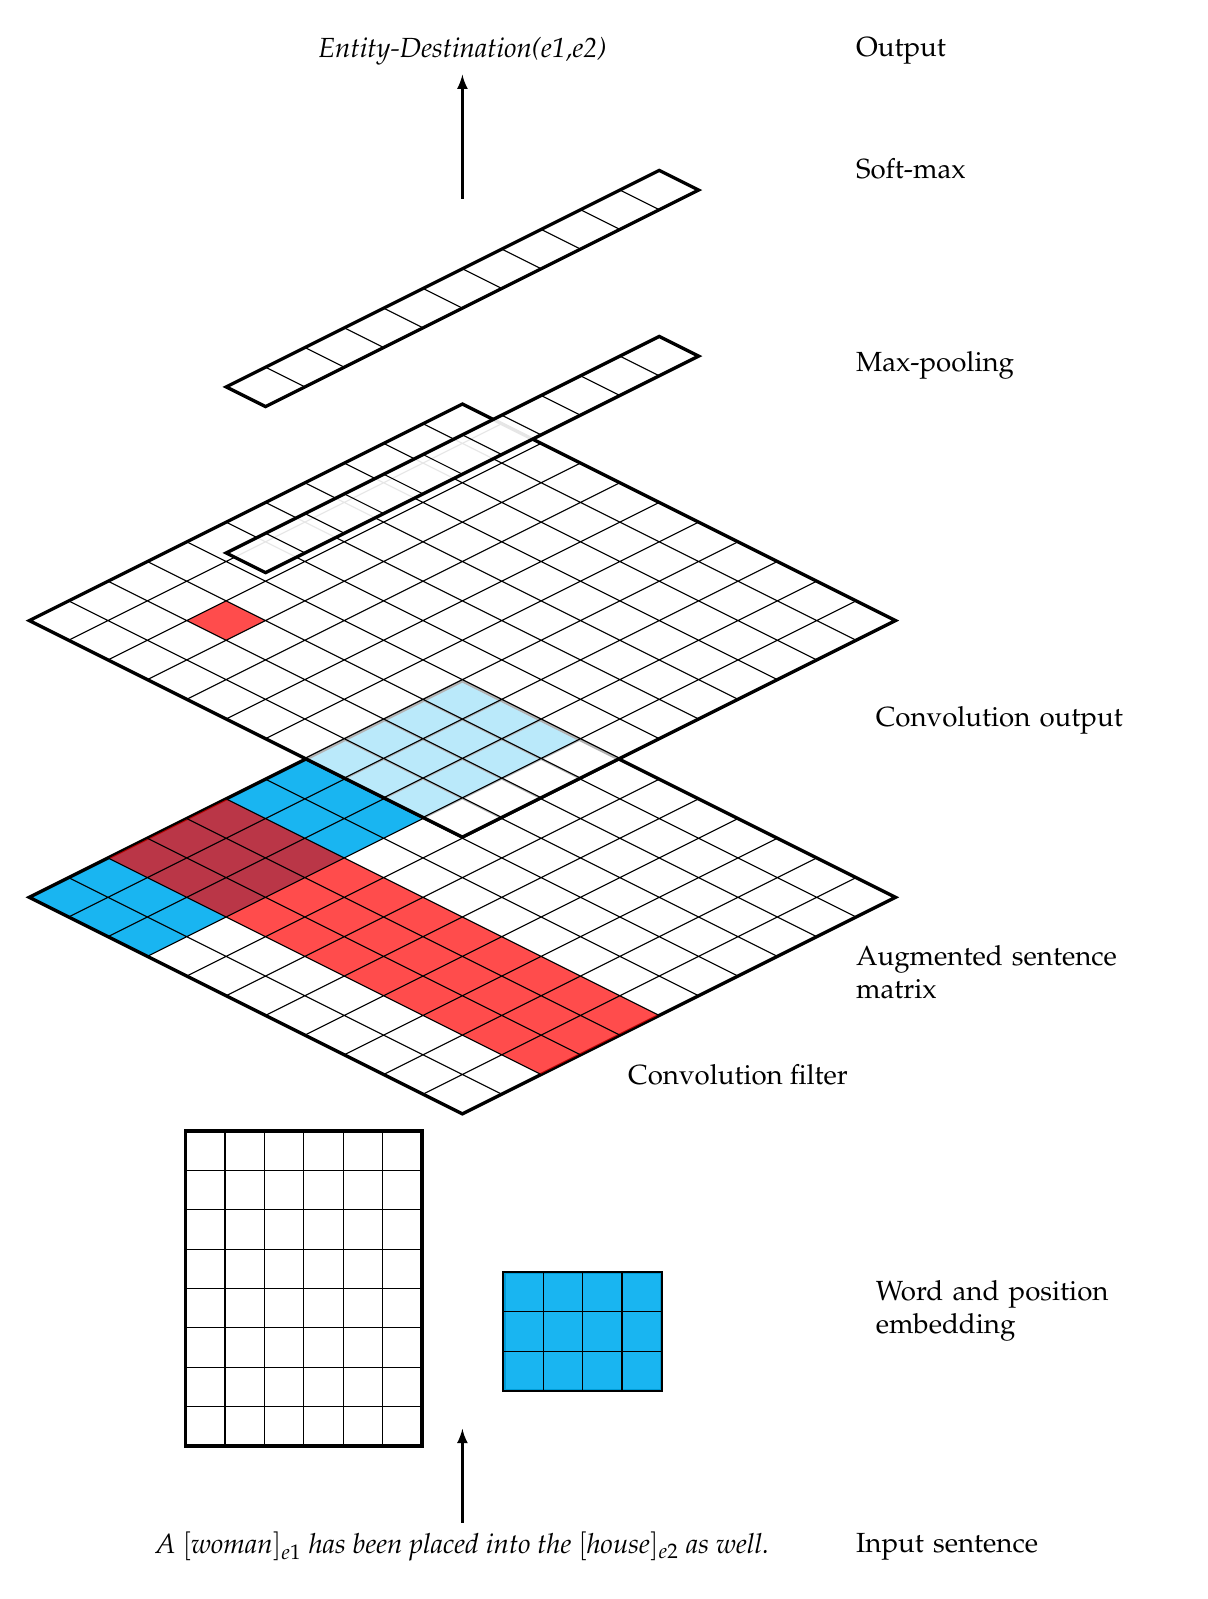
\begin{tikzpicture}[on grid]
    	\begin{scope}[yshift=0,
    				  every node/.append style={
	       	    	  	yslant=0.5,
    	    	        xslant=-1
		    	      },
    	              yslant=0.
    	              5,xslant=-1]
        	\fill[cyan,fill opacity=.9] (0,4) rectangle (5.5,5.5);
	        \draw[black,very thick] (0,0) rectangle (5.5,5.5);
	       	\fill[red,fill opacity=.7] (1,0) rectangle (2.5,5.5);
    	    \draw[step=5mm, black] (0,0) grid (5.5,5.5); 
    \end{scope}
   	\begin{scope}[yshift=100,
   				  every node/.append style={
   	    	  	    yslant=0.5,
    	    	    xslant=-1
		    	  },
    	          yslant=0.
    	          5,xslant=-1]
        	\fill[white,fill opacity=.7] (0,0) rectangle (5.5,5.5);
        	\fill[red,fill opacity=.7] (1,4.5) rectangle (1.5,4);
	        \draw[black,very thick] (0,0) rectangle (5.5,5.5);
    	    \draw[step=5mm, black] (0,0) grid (5.5,5.5);
    \end{scope}
    \begin{scope}[yshift=160,
    			  xshift=0,
    			  every node/.append style={
	       	      	yslant=0.5,
    	    	    xslant=-1
		    	  },
    	          yslant=0.
    	          5,xslant=-1]
        	\fill[white,fill opacity=.9] (0,3) rectangle (5.5,2.5);
	        \draw[black,very thick] (0,3) rectangle (5.5,2.5);
    	    \draw[step=5mm, black] (0,3) grid (5.5,2.5);
    \end{scope}
    \begin{scope}[yshift=220,
    			  xshift=0,
    			  every node/.append style={
	       	      	yslant=0.5,
    	    	    xslant=-1
		    	  },
    	          yslant=0.
    	          5,xslant=-1]
        	\fill[white,fill opacity=.9] (0,3) rectangle (5.5,2.5);
	        \draw[black,very thick] (0,3) rectangle (5.5,2.5);
    	    \draw[step=5mm, black] (0,3) grid (5.5,2.5);
    \end{scope}
    \begin{scope}[yshift=-120, xshift=-100]
    	\draw[black,very thick] (0,0) rectangle (3,4);
   	    \draw[step=5mm, black] (0,0) grid (3,4);    	
    \end{scope}
        \begin{scope}[yshift=-100, xshift=15]
    	\draw[black,very thick] (0,0) rectangle (2,1.5);
		\fill[cyan,fill opacity=.9] (0,0) rectangle (2,1.5);
   	    \draw[step=5mm, black] (0,0) grid (2,1.5);
    \end{scope}
    \node [text width=4cm] at (7,1.8) {Augmented sentence matrix};
    \node [text width=3.5cm] at (7,-2.5) {Word and position embedding};
    \node [text width=4cm] at (7,-5.5) {Input sentence};
    \node [] at (3.5,.5) {Convolution filter};
	\node [text width=3.5cm] at (7,5) {Convolution output};
	\node [text width=4cm] at (7,9.5) {Max-pooling};
	\node [text width=4cm] at (7,12) {Soft-max};
	\node [] (input) at (0,-5.5) {\textit{A $[$woman$]_{e1}$ has been placed into the $[$house$]_{e2}$ as well.}};
	\node [] (output) at (0,13.5) {\textit{Entity-Destination(e1,e2)}};
	\node [text width=4cm] at (7,13.5) {Output};
	\node [] (start) at (0,11.5) {};
	\draw [-latex, thick] (input) edge (0, -4);
	\draw [-latex, thick] (start) edge (output);	
	\end{tikzpicture}
	\caption{Diagram of convolutional neural network for relation classification. The input sentence is mapped to a sentence matrix by concatenating the word-vector for each word in the word embedding matrix and the position-vector for each word-position in the position embedding matrix. This forms an $s \times d + d'$ matrix. Convolution filters are applied along the $s$-axis of the sentence matrix to produce the convolution output. Each element in the convolution output matrix corresponds to one convolution filter applied at one position of the sentence matrix. Max-pooling is applied to the convolution output to obtain a feature-vector. This vector is used as input to a soft-max output layer.}
	\label{relation_architecture}
\end{figure}
For the relation classification tasks we use a state-of-the-art convolutional neural network architecture based on \citet{nguyen2015}. In this architecture, each word $s_i$ of an input sentence $s$ is first mapped to a word-vector $\vector{v}_i \in \mathbb{R}^d$ through a word-embedding matrix to form a sentence matrix $\vector{S}$. To ensure that the dimensionality of $\vector{S}$ is consistent across sentences, we compute the longest sentence length $K$ of the sentences in the SemEval and ACE corpora and pad shorter sentences with a padding token as a preprocessing step, such that $\vector{S} = [\vector{v}_1, \dots, \vector{v}_K]^T$.

To indicate which words in the input sentence are the head words of relation arguments, we compute the distance between each word index $i$ and the index of the head word of the relation arguments $e1$ and $e2$ as $i - e1$ and $i - e2$. These distances are mapped into real valued position vectors $\vector{p}_{1i}$ for the distance $i - e1$ for each word, and $\vector{P}_{2i}$ for the distance $i - e2$ for each word, both in  $\mathbb{R}^{d'}$. From these we construct the position matrices $\vector{P}_1 = [\vector{p}_{11},\dots,\vector{p}_{1K}]^T$ and $\vector{P}_2 = [\vector{p}_{21},\dots,\vector{p}_{2K}]^T$. We use the three matrices $\vector{S}$, $\vector{P}_1$ and $\vector{P}_2$ to form the augmented sentence matrix $\vector{S}' = [\vector{S} \mid \vector{P}_1 \mid \vector{P}_2] \in \mathbb{R}^{K \times (d + 2d')}$.
\\\\
The $K \times (d + 2d')$ dimensional augmented sentence matrix is used as input for a convolutional neural network layer. The convolution filters are applied over the full height of augmented sentence matrix in windows of $n$ tokens over the $K$ dimensional axis. In other words, each convolution filter is a weight matrix $\vector{W} \in \mathbb{R}^{n \times (d + 2d')}$. The output of the convolutional neural at position $i$ is:
$$
\sigma\left(w_0 + \sum\limits_{j = i}^{i + n}\vector{S}'_i\vector{W}_i^T\right)
$$
Where $\sigma$ is the ReLU activation function, $\vector{W}_i$ and $\vector{S}'_i$ is the $i$'th row of the convolutional filter matrix and augmented sentence matrix respectively, and $w_0$ is a bias term. In our experiment we use 150 filters of each window size, and window sizes $n$ of 2, 3, 4 and 5 for a total of 600 convolutional filters.

We apply max-pooling to the output of each convolutional filter yielding a 600 dimensional feature vector, which is used as input for a soft-max output layer. See figure \ref{relation_architecture} for a diagram.
\\\\
For the sequence classification tasks we use a convolutional neural network architecture based on \citet{collobert2011}. This architecture is virtually identical to the architecture used for the relation classification task. To predict the tag for word $s_i$ in the sentence $s$, a window of $K$ tokens around $s_i$ is transformed into a sentence matrix $\vector{S} = [\vector{v}_{i - \frac{K}{2}},\dots,\vector{v}_i,\dots,\vector{v}_{i + \frac{K}{2}}]^T \in \mathbb{R}^{K \times d}$ where $\vector{v}_i \in \mathbb{R}^d$ is taken from a word-embedding matrix. For words where $i \pm K / 2$ exceeds the sentence border a padding token is used. The sentence matrix $\vector{S}$ is used directly as input to the convolutional layer. In other words, the convolutional filter weights $\vector{W}$ for sequence classification tasks have dimensionality $n \times d$, where $n$ is the convolution filter window size.
\\\\
The subtle differences between the network architecture used for sequence and relation classification lead to some technical difficulties. Since most symbolic differentiation software used for neural network training such as TensorFlow or Theano use matrix-vector formulations, neural network weights must be expressed as matrices in these frameworks \citep{abadi2016, theano2016}. This means that the convolutional filter weights $\vector{W}$ cannot be shared between the sequence classification tasks and the relation classification tasks, since the filters have dimensionality $K \times d$ in one and $K \times d + 2d'$ in the other.
\\\\
For this reason, we share only the word-embedding matrix between the relation classification tasks and sequence classification tasks.
In our experiment, we initialize the word-embedding matrix with GloVe vectors trained on the Common Crawl corpus (commoncrawl.org). A diagram of neural network weights are shared between tasks can be seen in figure \ref{relation_sequence_weight_sharing}

\tikzstyle{box} = [rectangle, draw, node distance=3cm, align=center, minimum height=4em, minimum width=18em, thick]
\begin{figure}
	\centering
	\begin{tikzpicture}
		\node [box] (embedding) at (0,0) {Shared word-embedding matrix};
		\node [draw=none,rectangle, align=center, minimum height=4em, draw, thick, minimum width=10em] (position_embedding) at (-5.5,0) {position-embedding\\matrix};
		\node [draw=none,rectangle, align=center, minimum height=4em, draw, thick, minimum width=10em, dashed] (position_embedding2) at (5.5,0) {position-embedding\\matrix};
		\node [box] (convolutions_task1) at (4,4) {Convolutional filters and\\max-pooling};
		\node [box] (convolutions_task2) at (-4,4) {Convolutional filters and\\max-pooling};
		\node [box] (output_1) at (4,8) {Soft-max output};
		\node [box] (output_2) at (-4,8) {Soft-max output};
		\node [box] (aux_sentence) at (4,-4) {Auxiliary task input};
		\node [box] (target_sentence) at (-4,-4) {SemEval input};
		\draw[-latex, thick] (target_sentence) edge (embedding);
		\draw[-latex, thick] (target_sentence) edge (position_embedding);
		\draw[-latex, thick] (aux_sentence) edge (embedding);
		\draw[-latex, thick] (embedding) edge (convolutions_task1);
		\draw[-latex, thick] (embedding) edge (convolutions_task2);
		\draw[-latex, thick] (convolutions_task1) edge (output_1);
		\draw[-latex, thick] (convolutions_task2) edge (output_2);
		\draw[-latex, thick] (position_embedding) edge (convolutions_task2);
		\draw[-latex, thick, dashed] (aux_sentence) edge (position_embedding2);
		\draw[-latex, thick, dashed] (position_embedding2) edge (convolutions_task1);
	\end{tikzpicture}
	\caption{Diagram of how neural network weights are shared between auxiliary tasks and SemEval 2010 Task 8. The word-embedding matrix is shared between tasks, but the convolution filters are not.}
	\label{relation_sequence_weight_sharing}
\end{figure}
\section{Algorithm}

Our main goal is to investigate the sample complexity dynamics of learning a relation classification task in a multi-task learning setting. To this end, we compare the generalisation error of a deep learning model trained only on SemEval 2010 Task 8, the target task, with the generalisation error of a deep learning model trained jointly on the SemEval data and one of the auxiliary tasks described in \ref{auxiliary_tasks}.
\\\\
We proceed as follows: We vary the amount of data from the target task and auxiliary task in turn by a set of fractions. For every combination of fractional target and auxiliary data, we perform 5-fold cross validation on the target data to yield 5 macro-F1 scores. We use the training data from the 4 training folds of target data and the auxiliary data to train the architecture described in \ref{network_architecture}. This is done by uniformly selecting one of the two tasks, sampling a mini-batch of the fractional training data from that task, and performing one gradient descent update with respect to cross-entropy error using the Adam algorithm described in section \ref{adam}. 
\\\\
This process is iterated until an early stopping criterion on the target training data is met. Specifically, $1/10$ of target training data is set aside for early stopping validation. When the cross-entropy error on the early stopping dataset has not improved for 200 iterations of mini-batch gradient descent, training is halted, and the model weights are reset to their best recorded value.

When the patience is exceeded we record the cross-validation macro-F1 on the target task test fold using the best recorded weights. Since neural network training is a random search procedure with respect to weight initialization and mini-batch sampling, we run this experiment for each combination of target and auxiliary fractional data 5 times, yielding a total of 25 random cross-validation splits for each combination. We have provided the algorithm used in our experiments as pseudocode in algorithm \ref{experiment_pseudocode}.
\begin{algorithm}
\begin{algorithmic}
	\Require $miniBatchSize$: an integer giving the mini-batch size
	\Require $targetData = \{(\vector{x}_{t1},\vector{y}_{t1}),\dots,(\vector{x}_{tN},\vector{y}_{tN})\}$
	\Require $auxiliaryData = \{(\vector{x}_{a1},\vector{y}_{a1}),\dots,(\vector{x}_{aN},\vector{y}_{aN})\}$
	\Require $sample(data, fraction)$: A routine that can sample $|set| \cdot fraction$ samples from the set $data$ uniformly.
	\Require $crossValidation(data)$: A routine that returns a set of cross-validation folds over the set $data$.
	\Require $initializeWeights()$: A routine that can initialize a neural network weight vector.
	\Require $gradientDescent(data, w)$: A routine that performs gradient descent on the neural network weights $w$.
	\Require $macroF1(w, data)$: A routine that computes the macro F1 score on $data$ using neural network weights $w$.
	\Require $report(score, targetFraction, auxiliaryFraction)$: A reporting routine.
	\State $fractions \gets \{\frac{0}{5}, \frac{1}{5}, \frac{2}{5}, \frac{3}{5}, \frac{4}{5}, 1\}$
	\For{$iteration \in \{1,\dots,5\}$}
		\For{$targetFraction \in fractions$}
			\For{$auxiliaryFraction \in fractions$}
				\State $targetFractionalData \gets sample(targetData, targetFraction)$
				\State $auxiliaryFractionalData \gets sample(auxiliaryData, auxiliaryFraction)$
				\State $earlyStoppingData \gets sample(targetFractionalData, \frac{1}{10})$
				\State $targetTrainData = targetFractionalData \setminus earlyStoppingData$
				\For{$trainFold, testFold \in crossValidation(targetTrainData)$}
					\State $\vector{w} \gets initializeWeights()$
					\While{\textit{patience not exceeded}}
						\State $task \gets sample(\{trainFold, auxiliaryFractionalData\}, \frac{1}{2})$
						\State $miniBatch \gets sample(task, \frac{|task|}{miniBatchSize})$
						\State $\vector{w} \gets gradientDescent(miniBatch, \vector{w})$
					\EndWhile
					\State $score = macroF1(\vector{w}, testFold)$
					\State $report(score, targetFraction, auxiliaryFraction)$
				\EndFor
			\EndFor
		\EndFor
	\EndFor
\end{algorithmic}
\caption{Pseudocode for our deep multi-task learning experiment.}\label{experiment_pseudocode}
\end{algorithm}


\section{Summary}
In this section we have summarized the state of related work for deep multi-task learning for relation classification. We found that no previous investigation of the usefulness of deep multi-task learning for relation classification exists. 
\\\\
We have described the SemEval 2010 Task 8 dataset which we use as a benchmark in our experiments. In this context, we discussed the need for a benchmark dataset that gives us confidence about the generality of an experiment that uses it. We have called into question whether the SemEval dataset has this quality. Nevertheless, we have decided to use it as a benchmark in our experiments because of its status as the de facto standard dataset for relation classification experiments.
\\\\
Moreover, we have described each auxiliary task for which we test the impact of hard neural network weight sharing on the target task. Finally, we have described the neural network architectures used, and how we adapt them to enable weight sharing, as well as the algorithm used to train this architecture.
\\\\
We continue by presenting the results obtained from our experiments.
\chapter{Results}
In this section we present the results obtained in the experiment detailed in the previous sections. We visualize the effect of multi-task learning on generalization error estimated by cross-validation for each of the proposed weight sharing strategies. Specifically, we plot the mean macro F1 for each cross-validation experiment as a function of the fraction of target data available for training. This produces a so called \textbf{learning curve} that indicates how generalization error improves as the amount of training data is increased in both the single-task and multi-task setting.
\\\\
Moreover, we perform statistical tests of significance using one sided t-testing on the data collected for each fraction $f$ of target data in order to determine if the observed differences between single-task and multi-task learning can be explained by variation due to random weight initialization and and stochastic gradient descent.
\newpage
\section{Shared Embeddings}
\newpage
\section{Shared Side Channel Convolutional Filters}
In this section we present the results obtained for SemEval 2010 Task 8 in a single-task and multi-task setting using the multi-channel weight sharing strategy discussed in section \ref{network_architecture}. Each plot contains two curves: one learning curve for SemEval 2010 Task 8 when learnt as a single task, and one when learnt simultaneously with an auxiliary task. In addition we present tables containing the $p$-value of one-sided t-tests between the macro $F1$ scores of multi-task and single-task experiments grouped by the fraction of target data $f$.
\vspace{2cm}
\begin{figure}[h]
	\centering
	%% Creator: Matplotlib, PGF backend
%%
%% To include the figure in your LaTeX document, write
%%   \input{<filename>.pgf}
%%
%% Make sure the required packages are loaded in your preamble
%%   \usepackage{pgf}
%%
%% Figures using additional raster images can only be included by \input if
%% they are in the same directory as the main LaTeX file. For loading figures
%% from other directories you can use the `import` package
%%   \usepackage{import}
%% and then include the figures with
%%   \import{<path to file>}{<filename>.pgf}
%%
%% Matplotlib used the following preamble
%%   \usepackage{fontspec}
%%   \setmainfont{Palatino}
%%   \setsansfont{Lucida Grande}
%%   \setmonofont{Andale Mono}
%%
\begingroup%
\makeatletter%
\begin{pgfpicture}%
\pgfpathrectangle{\pgfpointorigin}{\pgfqpoint{5.004722in}{3.175278in}}%
\pgfusepath{use as bounding box, clip}%
\begin{pgfscope}%
\pgfsetbuttcap%
\pgfsetmiterjoin%
\definecolor{currentfill}{rgb}{1.000000,1.000000,1.000000}%
\pgfsetfillcolor{currentfill}%
\pgfsetlinewidth{0.000000pt}%
\definecolor{currentstroke}{rgb}{1.000000,1.000000,1.000000}%
\pgfsetstrokecolor{currentstroke}%
\pgfsetdash{}{0pt}%
\pgfpathmoveto{\pgfqpoint{0.000000in}{0.000000in}}%
\pgfpathlineto{\pgfqpoint{5.004722in}{0.000000in}}%
\pgfpathlineto{\pgfqpoint{5.004722in}{3.175278in}}%
\pgfpathlineto{\pgfqpoint{0.000000in}{3.175278in}}%
\pgfpathclose%
\pgfusepath{fill}%
\end{pgfscope}%
\begin{pgfscope}%
\pgfsetbuttcap%
\pgfsetmiterjoin%
\definecolor{currentfill}{rgb}{1.000000,1.000000,1.000000}%
\pgfsetfillcolor{currentfill}%
\pgfsetlinewidth{0.000000pt}%
\definecolor{currentstroke}{rgb}{0.000000,0.000000,0.000000}%
\pgfsetstrokecolor{currentstroke}%
\pgfsetstrokeopacity{0.000000}%
\pgfsetdash{}{0pt}%
\pgfpathmoveto{\pgfqpoint{0.430962in}{0.403645in}}%
\pgfpathlineto{\pgfqpoint{4.916179in}{0.403645in}}%
\pgfpathlineto{\pgfqpoint{4.916179in}{3.157778in}}%
\pgfpathlineto{\pgfqpoint{0.430962in}{3.157778in}}%
\pgfpathclose%
\pgfusepath{fill}%
\end{pgfscope}%
\begin{pgfscope}%
\pgfsetbuttcap%
\pgfsetroundjoin%
\definecolor{currentfill}{rgb}{0.000000,0.000000,0.000000}%
\pgfsetfillcolor{currentfill}%
\pgfsetlinewidth{0.803000pt}%
\definecolor{currentstroke}{rgb}{0.000000,0.000000,0.000000}%
\pgfsetstrokecolor{currentstroke}%
\pgfsetdash{}{0pt}%
\pgfsys@defobject{currentmarker}{\pgfqpoint{0.000000in}{-0.048611in}}{\pgfqpoint{0.000000in}{0.000000in}}{%
\pgfpathmoveto{\pgfqpoint{0.000000in}{0.000000in}}%
\pgfpathlineto{\pgfqpoint{0.000000in}{-0.048611in}}%
\pgfusepath{stroke,fill}%
}%
\begin{pgfscope}%
\pgfsys@transformshift{0.430962in}{0.403645in}%
\pgfsys@useobject{currentmarker}{}%
\end{pgfscope}%
\end{pgfscope}%
\begin{pgfscope}%
\pgftext[x=0.430962in,y=0.306423in,,top]{\rmfamily\fontsize{8.000000}{9.600000}\selectfont \(\displaystyle 0\)}%
\end{pgfscope}%
\begin{pgfscope}%
\pgfsetbuttcap%
\pgfsetroundjoin%
\definecolor{currentfill}{rgb}{0.000000,0.000000,0.000000}%
\pgfsetfillcolor{currentfill}%
\pgfsetlinewidth{0.803000pt}%
\definecolor{currentstroke}{rgb}{0.000000,0.000000,0.000000}%
\pgfsetstrokecolor{currentstroke}%
\pgfsetdash{}{0pt}%
\pgfsys@defobject{currentmarker}{\pgfqpoint{0.000000in}{-0.048611in}}{\pgfqpoint{0.000000in}{0.000000in}}{%
\pgfpathmoveto{\pgfqpoint{0.000000in}{0.000000in}}%
\pgfpathlineto{\pgfqpoint{0.000000in}{-0.048611in}}%
\pgfusepath{stroke,fill}%
}%
\begin{pgfscope}%
\pgfsys@transformshift{1.328006in}{0.403645in}%
\pgfsys@useobject{currentmarker}{}%
\end{pgfscope}%
\end{pgfscope}%
\begin{pgfscope}%
\pgftext[x=1.328006in,y=0.306423in,,top]{\rmfamily\fontsize{8.000000}{9.600000}\selectfont \(\displaystyle 20\)}%
\end{pgfscope}%
\begin{pgfscope}%
\pgfsetbuttcap%
\pgfsetroundjoin%
\definecolor{currentfill}{rgb}{0.000000,0.000000,0.000000}%
\pgfsetfillcolor{currentfill}%
\pgfsetlinewidth{0.803000pt}%
\definecolor{currentstroke}{rgb}{0.000000,0.000000,0.000000}%
\pgfsetstrokecolor{currentstroke}%
\pgfsetdash{}{0pt}%
\pgfsys@defobject{currentmarker}{\pgfqpoint{0.000000in}{-0.048611in}}{\pgfqpoint{0.000000in}{0.000000in}}{%
\pgfpathmoveto{\pgfqpoint{0.000000in}{0.000000in}}%
\pgfpathlineto{\pgfqpoint{0.000000in}{-0.048611in}}%
\pgfusepath{stroke,fill}%
}%
\begin{pgfscope}%
\pgfsys@transformshift{2.225049in}{0.403645in}%
\pgfsys@useobject{currentmarker}{}%
\end{pgfscope}%
\end{pgfscope}%
\begin{pgfscope}%
\pgftext[x=2.225049in,y=0.306423in,,top]{\rmfamily\fontsize{8.000000}{9.600000}\selectfont \(\displaystyle 40\)}%
\end{pgfscope}%
\begin{pgfscope}%
\pgfsetbuttcap%
\pgfsetroundjoin%
\definecolor{currentfill}{rgb}{0.000000,0.000000,0.000000}%
\pgfsetfillcolor{currentfill}%
\pgfsetlinewidth{0.803000pt}%
\definecolor{currentstroke}{rgb}{0.000000,0.000000,0.000000}%
\pgfsetstrokecolor{currentstroke}%
\pgfsetdash{}{0pt}%
\pgfsys@defobject{currentmarker}{\pgfqpoint{0.000000in}{-0.048611in}}{\pgfqpoint{0.000000in}{0.000000in}}{%
\pgfpathmoveto{\pgfqpoint{0.000000in}{0.000000in}}%
\pgfpathlineto{\pgfqpoint{0.000000in}{-0.048611in}}%
\pgfusepath{stroke,fill}%
}%
\begin{pgfscope}%
\pgfsys@transformshift{3.122092in}{0.403645in}%
\pgfsys@useobject{currentmarker}{}%
\end{pgfscope}%
\end{pgfscope}%
\begin{pgfscope}%
\pgftext[x=3.122092in,y=0.306423in,,top]{\rmfamily\fontsize{8.000000}{9.600000}\selectfont \(\displaystyle 60\)}%
\end{pgfscope}%
\begin{pgfscope}%
\pgfsetbuttcap%
\pgfsetroundjoin%
\definecolor{currentfill}{rgb}{0.000000,0.000000,0.000000}%
\pgfsetfillcolor{currentfill}%
\pgfsetlinewidth{0.803000pt}%
\definecolor{currentstroke}{rgb}{0.000000,0.000000,0.000000}%
\pgfsetstrokecolor{currentstroke}%
\pgfsetdash{}{0pt}%
\pgfsys@defobject{currentmarker}{\pgfqpoint{0.000000in}{-0.048611in}}{\pgfqpoint{0.000000in}{0.000000in}}{%
\pgfpathmoveto{\pgfqpoint{0.000000in}{0.000000in}}%
\pgfpathlineto{\pgfqpoint{0.000000in}{-0.048611in}}%
\pgfusepath{stroke,fill}%
}%
\begin{pgfscope}%
\pgfsys@transformshift{4.019135in}{0.403645in}%
\pgfsys@useobject{currentmarker}{}%
\end{pgfscope}%
\end{pgfscope}%
\begin{pgfscope}%
\pgftext[x=4.019135in,y=0.306423in,,top]{\rmfamily\fontsize{8.000000}{9.600000}\selectfont \(\displaystyle 80\)}%
\end{pgfscope}%
\begin{pgfscope}%
\pgfsetbuttcap%
\pgfsetroundjoin%
\definecolor{currentfill}{rgb}{0.000000,0.000000,0.000000}%
\pgfsetfillcolor{currentfill}%
\pgfsetlinewidth{0.803000pt}%
\definecolor{currentstroke}{rgb}{0.000000,0.000000,0.000000}%
\pgfsetstrokecolor{currentstroke}%
\pgfsetdash{}{0pt}%
\pgfsys@defobject{currentmarker}{\pgfqpoint{0.000000in}{-0.048611in}}{\pgfqpoint{0.000000in}{0.000000in}}{%
\pgfpathmoveto{\pgfqpoint{0.000000in}{0.000000in}}%
\pgfpathlineto{\pgfqpoint{0.000000in}{-0.048611in}}%
\pgfusepath{stroke,fill}%
}%
\begin{pgfscope}%
\pgfsys@transformshift{4.916179in}{0.403645in}%
\pgfsys@useobject{currentmarker}{}%
\end{pgfscope}%
\end{pgfscope}%
\begin{pgfscope}%
\pgftext[x=4.916179in,y=0.306423in,,top]{\rmfamily\fontsize{8.000000}{9.600000}\selectfont \(\displaystyle 100\)}%
\end{pgfscope}%
\begin{pgfscope}%
\pgftext[x=2.673571in,y=0.139431in,,top]{\rmfamily\fontsize{10.000000}{12.000000}\selectfont percentage of \(\displaystyle \mathcal{D}_t\)}%
\end{pgfscope}%
\begin{pgfscope}%
\pgfsetbuttcap%
\pgfsetroundjoin%
\definecolor{currentfill}{rgb}{0.000000,0.000000,0.000000}%
\pgfsetfillcolor{currentfill}%
\pgfsetlinewidth{0.803000pt}%
\definecolor{currentstroke}{rgb}{0.000000,0.000000,0.000000}%
\pgfsetstrokecolor{currentstroke}%
\pgfsetdash{}{0pt}%
\pgfsys@defobject{currentmarker}{\pgfqpoint{-0.048611in}{0.000000in}}{\pgfqpoint{0.000000in}{0.000000in}}{%
\pgfpathmoveto{\pgfqpoint{0.000000in}{0.000000in}}%
\pgfpathlineto{\pgfqpoint{-0.048611in}{0.000000in}}%
\pgfusepath{stroke,fill}%
}%
\begin{pgfscope}%
\pgfsys@transformshift{0.430962in}{0.702564in}%
\pgfsys@useobject{currentmarker}{}%
\end{pgfscope}%
\end{pgfscope}%
\begin{pgfscope}%
\pgftext[x=0.194851in,y=0.662145in,left,base]{\rmfamily\fontsize{8.000000}{9.600000}\selectfont 0.1}%
\end{pgfscope}%
\begin{pgfscope}%
\pgfsetbuttcap%
\pgfsetroundjoin%
\definecolor{currentfill}{rgb}{0.000000,0.000000,0.000000}%
\pgfsetfillcolor{currentfill}%
\pgfsetlinewidth{0.803000pt}%
\definecolor{currentstroke}{rgb}{0.000000,0.000000,0.000000}%
\pgfsetstrokecolor{currentstroke}%
\pgfsetdash{}{0pt}%
\pgfsys@defobject{currentmarker}{\pgfqpoint{-0.048611in}{0.000000in}}{\pgfqpoint{0.000000in}{0.000000in}}{%
\pgfpathmoveto{\pgfqpoint{0.000000in}{0.000000in}}%
\pgfpathlineto{\pgfqpoint{-0.048611in}{0.000000in}}%
\pgfusepath{stroke,fill}%
}%
\begin{pgfscope}%
\pgfsys@transformshift{0.430962in}{1.095135in}%
\pgfsys@useobject{currentmarker}{}%
\end{pgfscope}%
\end{pgfscope}%
\begin{pgfscope}%
\pgftext[x=0.194851in,y=1.054716in,left,base]{\rmfamily\fontsize{8.000000}{9.600000}\selectfont 0.2}%
\end{pgfscope}%
\begin{pgfscope}%
\pgfsetbuttcap%
\pgfsetroundjoin%
\definecolor{currentfill}{rgb}{0.000000,0.000000,0.000000}%
\pgfsetfillcolor{currentfill}%
\pgfsetlinewidth{0.803000pt}%
\definecolor{currentstroke}{rgb}{0.000000,0.000000,0.000000}%
\pgfsetstrokecolor{currentstroke}%
\pgfsetdash{}{0pt}%
\pgfsys@defobject{currentmarker}{\pgfqpoint{-0.048611in}{0.000000in}}{\pgfqpoint{0.000000in}{0.000000in}}{%
\pgfpathmoveto{\pgfqpoint{0.000000in}{0.000000in}}%
\pgfpathlineto{\pgfqpoint{-0.048611in}{0.000000in}}%
\pgfusepath{stroke,fill}%
}%
\begin{pgfscope}%
\pgfsys@transformshift{0.430962in}{1.487706in}%
\pgfsys@useobject{currentmarker}{}%
\end{pgfscope}%
\end{pgfscope}%
\begin{pgfscope}%
\pgftext[x=0.194851in,y=1.447287in,left,base]{\rmfamily\fontsize{8.000000}{9.600000}\selectfont 0.3}%
\end{pgfscope}%
\begin{pgfscope}%
\pgfsetbuttcap%
\pgfsetroundjoin%
\definecolor{currentfill}{rgb}{0.000000,0.000000,0.000000}%
\pgfsetfillcolor{currentfill}%
\pgfsetlinewidth{0.803000pt}%
\definecolor{currentstroke}{rgb}{0.000000,0.000000,0.000000}%
\pgfsetstrokecolor{currentstroke}%
\pgfsetdash{}{0pt}%
\pgfsys@defobject{currentmarker}{\pgfqpoint{-0.048611in}{0.000000in}}{\pgfqpoint{0.000000in}{0.000000in}}{%
\pgfpathmoveto{\pgfqpoint{0.000000in}{0.000000in}}%
\pgfpathlineto{\pgfqpoint{-0.048611in}{0.000000in}}%
\pgfusepath{stroke,fill}%
}%
\begin{pgfscope}%
\pgfsys@transformshift{0.430962in}{1.880276in}%
\pgfsys@useobject{currentmarker}{}%
\end{pgfscope}%
\end{pgfscope}%
\begin{pgfscope}%
\pgftext[x=0.194851in,y=1.839858in,left,base]{\rmfamily\fontsize{8.000000}{9.600000}\selectfont 0.4}%
\end{pgfscope}%
\begin{pgfscope}%
\pgfsetbuttcap%
\pgfsetroundjoin%
\definecolor{currentfill}{rgb}{0.000000,0.000000,0.000000}%
\pgfsetfillcolor{currentfill}%
\pgfsetlinewidth{0.803000pt}%
\definecolor{currentstroke}{rgb}{0.000000,0.000000,0.000000}%
\pgfsetstrokecolor{currentstroke}%
\pgfsetdash{}{0pt}%
\pgfsys@defobject{currentmarker}{\pgfqpoint{-0.048611in}{0.000000in}}{\pgfqpoint{0.000000in}{0.000000in}}{%
\pgfpathmoveto{\pgfqpoint{0.000000in}{0.000000in}}%
\pgfpathlineto{\pgfqpoint{-0.048611in}{0.000000in}}%
\pgfusepath{stroke,fill}%
}%
\begin{pgfscope}%
\pgfsys@transformshift{0.430962in}{2.272847in}%
\pgfsys@useobject{currentmarker}{}%
\end{pgfscope}%
\end{pgfscope}%
\begin{pgfscope}%
\pgftext[x=0.194851in,y=2.232429in,left,base]{\rmfamily\fontsize{8.000000}{9.600000}\selectfont 0.5}%
\end{pgfscope}%
\begin{pgfscope}%
\pgfsetbuttcap%
\pgfsetroundjoin%
\definecolor{currentfill}{rgb}{0.000000,0.000000,0.000000}%
\pgfsetfillcolor{currentfill}%
\pgfsetlinewidth{0.803000pt}%
\definecolor{currentstroke}{rgb}{0.000000,0.000000,0.000000}%
\pgfsetstrokecolor{currentstroke}%
\pgfsetdash{}{0pt}%
\pgfsys@defobject{currentmarker}{\pgfqpoint{-0.048611in}{0.000000in}}{\pgfqpoint{0.000000in}{0.000000in}}{%
\pgfpathmoveto{\pgfqpoint{0.000000in}{0.000000in}}%
\pgfpathlineto{\pgfqpoint{-0.048611in}{0.000000in}}%
\pgfusepath{stroke,fill}%
}%
\begin{pgfscope}%
\pgfsys@transformshift{0.430962in}{2.665418in}%
\pgfsys@useobject{currentmarker}{}%
\end{pgfscope}%
\end{pgfscope}%
\begin{pgfscope}%
\pgftext[x=0.194851in,y=2.624999in,left,base]{\rmfamily\fontsize{8.000000}{9.600000}\selectfont 0.6}%
\end{pgfscope}%
\begin{pgfscope}%
\pgfsetbuttcap%
\pgfsetroundjoin%
\definecolor{currentfill}{rgb}{0.000000,0.000000,0.000000}%
\pgfsetfillcolor{currentfill}%
\pgfsetlinewidth{0.803000pt}%
\definecolor{currentstroke}{rgb}{0.000000,0.000000,0.000000}%
\pgfsetstrokecolor{currentstroke}%
\pgfsetdash{}{0pt}%
\pgfsys@defobject{currentmarker}{\pgfqpoint{-0.048611in}{0.000000in}}{\pgfqpoint{0.000000in}{0.000000in}}{%
\pgfpathmoveto{\pgfqpoint{0.000000in}{0.000000in}}%
\pgfpathlineto{\pgfqpoint{-0.048611in}{0.000000in}}%
\pgfusepath{stroke,fill}%
}%
\begin{pgfscope}%
\pgfsys@transformshift{0.430962in}{3.057989in}%
\pgfsys@useobject{currentmarker}{}%
\end{pgfscope}%
\end{pgfscope}%
\begin{pgfscope}%
\pgftext[x=0.194851in,y=3.017570in,left,base]{\rmfamily\fontsize{8.000000}{9.600000}\selectfont 0.7}%
\end{pgfscope}%
\begin{pgfscope}%
\pgftext[x=0.139296in,y=1.780712in,,bottom,rotate=90.000000]{\rmfamily\fontsize{10.000000}{12.000000}\selectfont Mean macro F1}%
\end{pgfscope}%
\begin{pgfscope}%
\pgfpathrectangle{\pgfqpoint{0.430962in}{0.403645in}}{\pgfqpoint{4.485217in}{2.754132in}} %
\pgfusepath{clip}%
\pgfsetrectcap%
\pgfsetroundjoin%
\pgfsetlinewidth{1.505625pt}%
\definecolor{currentstroke}{rgb}{0.121569,0.466667,0.705882}%
\pgfsetstrokecolor{currentstroke}%
\pgfsetdash{}{0pt}%
\pgfpathmoveto{\pgfqpoint{0.430962in}{0.528833in}}%
\pgfpathlineto{\pgfqpoint{1.328006in}{2.690585in}}%
\pgfpathlineto{\pgfqpoint{2.225049in}{2.870213in}}%
\pgfpathlineto{\pgfqpoint{3.122092in}{2.927016in}}%
\pgfpathlineto{\pgfqpoint{4.019135in}{2.946813in}}%
\pgfpathlineto{\pgfqpoint{4.916179in}{2.989337in}}%
\pgfusepath{stroke}%
\end{pgfscope}%
\begin{pgfscope}%
\pgfpathrectangle{\pgfqpoint{0.430962in}{0.403645in}}{\pgfqpoint{4.485217in}{2.754132in}} %
\pgfusepath{clip}%
\pgfsetbuttcap%
\pgfsetroundjoin%
\pgfsetlinewidth{1.505625pt}%
\definecolor{currentstroke}{rgb}{1.000000,0.498039,0.054902}%
\pgfsetstrokecolor{currentstroke}%
\pgfsetdash{{5.550000pt}{2.400000pt}}{0.000000pt}%
\pgfpathmoveto{\pgfqpoint{0.430962in}{0.537862in}}%
\pgfpathlineto{\pgfqpoint{1.328006in}{2.710362in}}%
\pgfpathlineto{\pgfqpoint{2.225049in}{2.883755in}}%
\pgfpathlineto{\pgfqpoint{3.122092in}{2.983473in}}%
\pgfpathlineto{\pgfqpoint{4.019135in}{3.032590in}}%
\pgfpathlineto{\pgfqpoint{4.916179in}{3.001802in}}%
\pgfusepath{stroke}%
\end{pgfscope}%
\begin{pgfscope}%
\pgfsetrectcap%
\pgfsetmiterjoin%
\pgfsetlinewidth{0.501875pt}%
\definecolor{currentstroke}{rgb}{0.000000,0.000000,0.000000}%
\pgfsetstrokecolor{currentstroke}%
\pgfsetdash{}{0pt}%
\pgfpathmoveto{\pgfqpoint{0.430962in}{0.403645in}}%
\pgfpathlineto{\pgfqpoint{0.430962in}{3.157778in}}%
\pgfusepath{stroke}%
\end{pgfscope}%
\begin{pgfscope}%
\pgfsetrectcap%
\pgfsetmiterjoin%
\pgfsetlinewidth{0.501875pt}%
\definecolor{currentstroke}{rgb}{0.000000,0.000000,0.000000}%
\pgfsetstrokecolor{currentstroke}%
\pgfsetdash{}{0pt}%
\pgfpathmoveto{\pgfqpoint{0.430962in}{0.403645in}}%
\pgfpathlineto{\pgfqpoint{4.916179in}{0.403645in}}%
\pgfusepath{stroke}%
\end{pgfscope}%
\begin{pgfscope}%
\pgfsetrectcap%
\pgfsetroundjoin%
\pgfsetlinewidth{1.505625pt}%
\definecolor{currentstroke}{rgb}{0.121569,0.466667,0.705882}%
\pgfsetstrokecolor{currentstroke}%
\pgfsetdash{}{0pt}%
\pgfpathmoveto{\pgfqpoint{3.315617in}{0.782185in}}%
\pgfpathlineto{\pgfqpoint{3.565617in}{0.782185in}}%
\pgfusepath{stroke}%
\end{pgfscope}%
\begin{pgfscope}%
\pgftext[x=3.665617in,y=0.738435in,left,base]{\rmfamily\fontsize{9.000000}{10.800000}\selectfont SemEval 2010 Task 8}%
\end{pgfscope}%
\begin{pgfscope}%
\pgfsetbuttcap%
\pgfsetroundjoin%
\pgfsetlinewidth{1.505625pt}%
\definecolor{currentstroke}{rgb}{1.000000,0.498039,0.054902}%
\pgfsetstrokecolor{currentstroke}%
\pgfsetdash{{5.550000pt}{2.400000pt}}{0.000000pt}%
\pgfpathmoveto{\pgfqpoint{3.315617in}{0.594319in}}%
\pgfpathlineto{\pgfqpoint{3.565617in}{0.594319in}}%
\pgfusepath{stroke}%
\end{pgfscope}%
\begin{pgfscope}%
\pgftext[x=3.665617in,y=0.550569in,left,base]{\rmfamily\fontsize{9.000000}{10.800000}\selectfont +ACE 2005}%
\end{pgfscope}%
\end{pgfpicture}%
\makeatother%
\endgroup%

	
	\vspace*{1cm}
	
	\begin{tabular}{r | l | l | l | l | l | l}
		\textbf{Percentage of $\data_t$} & 0 & 20 & 40 & 60 & 80 & 100 \\  \hline
		\textbf{Mean single-task macro $F1$} & .056 & .606 & .652 & .667 & .672 & .683\\
		\textbf{Mean multi-task macro $F1$} & 0 & 0 & 0 & 0 & 0 & 0\\
		$p$\textbf{-value} & 0 & 0 & 0 & 0 & 0 & 0
	\end{tabular}
	\caption{Learning curves and hypothesis tests for SemEval 2010 Task 8 trained as a single task and in a multi-task setting with ACE 2005. The learning curves indicate a slight improvement of multi-task learning over single-task learning in the 60-80\% range}
\end{figure}
\begin{figure}
	\centering
	\input{img/shared_filters_Conll2000POS_learning_curve.pgf}
	\vspace*{1cm}
	
	\begin{tabular}{r | l | l | l | l | l | l}
		\textbf{Percentage of $\data_t$} & 0 & 20 & 40 & 60 & 80 & 100 \\  \hline
		\textbf{Mean single-task macro $F1$} & .056 & .606 & .652 & .667 & .672 & .683\\
		\textbf{Mean multi-task macro $F1$} & 0 & 0 & 0 & 0 & 0 & 0\\
		$p$\textbf{-value} & 0 & 0 & 0 & 0 & 0 & 0
	\end{tabular}
	\caption{Learning curves and hypothesis tests for SemEval 2010 Task 8 trained as a single task and in a multi-task setting with CONLL2000 part-of-speech. The learning curves indicate a slight improvement of multi-task learning over single-task learning in the 60-80\% range}
\end{figure}
\begin{figure}
	\centering
	%% Creator: Matplotlib, PGF backend
%%
%% To include the figure in your LaTeX document, write
%%   \input{<filename>.pgf}
%%
%% Make sure the required packages are loaded in your preamble
%%   \usepackage{pgf}
%%
%% Figures using additional raster images can only be included by \input if
%% they are in the same directory as the main LaTeX file. For loading figures
%% from other directories you can use the `import` package
%%   \usepackage{import}
%% and then include the figures with
%%   \import{<path to file>}{<filename>.pgf}
%%
%% Matplotlib used the following preamble
%%   \usepackage{fontspec}
%%   \setmainfont{Palatino}
%%   \setsansfont{Lucida Grande}
%%   \setmonofont{Andale Mono}
%%
\begingroup%
\makeatletter%
\begin{pgfpicture}%
\pgfpathrectangle{\pgfpointorigin}{\pgfqpoint{5.004722in}{3.175278in}}%
\pgfusepath{use as bounding box, clip}%
\begin{pgfscope}%
\pgfsetbuttcap%
\pgfsetmiterjoin%
\definecolor{currentfill}{rgb}{1.000000,1.000000,1.000000}%
\pgfsetfillcolor{currentfill}%
\pgfsetlinewidth{0.000000pt}%
\definecolor{currentstroke}{rgb}{1.000000,1.000000,1.000000}%
\pgfsetstrokecolor{currentstroke}%
\pgfsetdash{}{0pt}%
\pgfpathmoveto{\pgfqpoint{0.000000in}{0.000000in}}%
\pgfpathlineto{\pgfqpoint{5.004722in}{0.000000in}}%
\pgfpathlineto{\pgfqpoint{5.004722in}{3.175278in}}%
\pgfpathlineto{\pgfqpoint{0.000000in}{3.175278in}}%
\pgfpathclose%
\pgfusepath{fill}%
\end{pgfscope}%
\begin{pgfscope}%
\pgfsetbuttcap%
\pgfsetmiterjoin%
\definecolor{currentfill}{rgb}{1.000000,1.000000,1.000000}%
\pgfsetfillcolor{currentfill}%
\pgfsetlinewidth{0.000000pt}%
\definecolor{currentstroke}{rgb}{0.000000,0.000000,0.000000}%
\pgfsetstrokecolor{currentstroke}%
\pgfsetstrokeopacity{0.000000}%
\pgfsetdash{}{0pt}%
\pgfpathmoveto{\pgfqpoint{0.430962in}{0.403645in}}%
\pgfpathlineto{\pgfqpoint{4.916179in}{0.403645in}}%
\pgfpathlineto{\pgfqpoint{4.916179in}{3.157778in}}%
\pgfpathlineto{\pgfqpoint{0.430962in}{3.157778in}}%
\pgfpathclose%
\pgfusepath{fill}%
\end{pgfscope}%
\begin{pgfscope}%
\pgfsetbuttcap%
\pgfsetroundjoin%
\definecolor{currentfill}{rgb}{0.000000,0.000000,0.000000}%
\pgfsetfillcolor{currentfill}%
\pgfsetlinewidth{0.803000pt}%
\definecolor{currentstroke}{rgb}{0.000000,0.000000,0.000000}%
\pgfsetstrokecolor{currentstroke}%
\pgfsetdash{}{0pt}%
\pgfsys@defobject{currentmarker}{\pgfqpoint{0.000000in}{-0.048611in}}{\pgfqpoint{0.000000in}{0.000000in}}{%
\pgfpathmoveto{\pgfqpoint{0.000000in}{0.000000in}}%
\pgfpathlineto{\pgfqpoint{0.000000in}{-0.048611in}}%
\pgfusepath{stroke,fill}%
}%
\begin{pgfscope}%
\pgfsys@transformshift{0.430962in}{0.403645in}%
\pgfsys@useobject{currentmarker}{}%
\end{pgfscope}%
\end{pgfscope}%
\begin{pgfscope}%
\pgftext[x=0.430962in,y=0.306423in,,top]{\rmfamily\fontsize{8.000000}{9.600000}\selectfont \(\displaystyle 0\)}%
\end{pgfscope}%
\begin{pgfscope}%
\pgfsetbuttcap%
\pgfsetroundjoin%
\definecolor{currentfill}{rgb}{0.000000,0.000000,0.000000}%
\pgfsetfillcolor{currentfill}%
\pgfsetlinewidth{0.803000pt}%
\definecolor{currentstroke}{rgb}{0.000000,0.000000,0.000000}%
\pgfsetstrokecolor{currentstroke}%
\pgfsetdash{}{0pt}%
\pgfsys@defobject{currentmarker}{\pgfqpoint{0.000000in}{-0.048611in}}{\pgfqpoint{0.000000in}{0.000000in}}{%
\pgfpathmoveto{\pgfqpoint{0.000000in}{0.000000in}}%
\pgfpathlineto{\pgfqpoint{0.000000in}{-0.048611in}}%
\pgfusepath{stroke,fill}%
}%
\begin{pgfscope}%
\pgfsys@transformshift{1.328006in}{0.403645in}%
\pgfsys@useobject{currentmarker}{}%
\end{pgfscope}%
\end{pgfscope}%
\begin{pgfscope}%
\pgftext[x=1.328006in,y=0.306423in,,top]{\rmfamily\fontsize{8.000000}{9.600000}\selectfont \(\displaystyle 20\)}%
\end{pgfscope}%
\begin{pgfscope}%
\pgfsetbuttcap%
\pgfsetroundjoin%
\definecolor{currentfill}{rgb}{0.000000,0.000000,0.000000}%
\pgfsetfillcolor{currentfill}%
\pgfsetlinewidth{0.803000pt}%
\definecolor{currentstroke}{rgb}{0.000000,0.000000,0.000000}%
\pgfsetstrokecolor{currentstroke}%
\pgfsetdash{}{0pt}%
\pgfsys@defobject{currentmarker}{\pgfqpoint{0.000000in}{-0.048611in}}{\pgfqpoint{0.000000in}{0.000000in}}{%
\pgfpathmoveto{\pgfqpoint{0.000000in}{0.000000in}}%
\pgfpathlineto{\pgfqpoint{0.000000in}{-0.048611in}}%
\pgfusepath{stroke,fill}%
}%
\begin{pgfscope}%
\pgfsys@transformshift{2.225049in}{0.403645in}%
\pgfsys@useobject{currentmarker}{}%
\end{pgfscope}%
\end{pgfscope}%
\begin{pgfscope}%
\pgftext[x=2.225049in,y=0.306423in,,top]{\rmfamily\fontsize{8.000000}{9.600000}\selectfont \(\displaystyle 40\)}%
\end{pgfscope}%
\begin{pgfscope}%
\pgfsetbuttcap%
\pgfsetroundjoin%
\definecolor{currentfill}{rgb}{0.000000,0.000000,0.000000}%
\pgfsetfillcolor{currentfill}%
\pgfsetlinewidth{0.803000pt}%
\definecolor{currentstroke}{rgb}{0.000000,0.000000,0.000000}%
\pgfsetstrokecolor{currentstroke}%
\pgfsetdash{}{0pt}%
\pgfsys@defobject{currentmarker}{\pgfqpoint{0.000000in}{-0.048611in}}{\pgfqpoint{0.000000in}{0.000000in}}{%
\pgfpathmoveto{\pgfqpoint{0.000000in}{0.000000in}}%
\pgfpathlineto{\pgfqpoint{0.000000in}{-0.048611in}}%
\pgfusepath{stroke,fill}%
}%
\begin{pgfscope}%
\pgfsys@transformshift{3.122092in}{0.403645in}%
\pgfsys@useobject{currentmarker}{}%
\end{pgfscope}%
\end{pgfscope}%
\begin{pgfscope}%
\pgftext[x=3.122092in,y=0.306423in,,top]{\rmfamily\fontsize{8.000000}{9.600000}\selectfont \(\displaystyle 60\)}%
\end{pgfscope}%
\begin{pgfscope}%
\pgfsetbuttcap%
\pgfsetroundjoin%
\definecolor{currentfill}{rgb}{0.000000,0.000000,0.000000}%
\pgfsetfillcolor{currentfill}%
\pgfsetlinewidth{0.803000pt}%
\definecolor{currentstroke}{rgb}{0.000000,0.000000,0.000000}%
\pgfsetstrokecolor{currentstroke}%
\pgfsetdash{}{0pt}%
\pgfsys@defobject{currentmarker}{\pgfqpoint{0.000000in}{-0.048611in}}{\pgfqpoint{0.000000in}{0.000000in}}{%
\pgfpathmoveto{\pgfqpoint{0.000000in}{0.000000in}}%
\pgfpathlineto{\pgfqpoint{0.000000in}{-0.048611in}}%
\pgfusepath{stroke,fill}%
}%
\begin{pgfscope}%
\pgfsys@transformshift{4.019135in}{0.403645in}%
\pgfsys@useobject{currentmarker}{}%
\end{pgfscope}%
\end{pgfscope}%
\begin{pgfscope}%
\pgftext[x=4.019135in,y=0.306423in,,top]{\rmfamily\fontsize{8.000000}{9.600000}\selectfont \(\displaystyle 80\)}%
\end{pgfscope}%
\begin{pgfscope}%
\pgfsetbuttcap%
\pgfsetroundjoin%
\definecolor{currentfill}{rgb}{0.000000,0.000000,0.000000}%
\pgfsetfillcolor{currentfill}%
\pgfsetlinewidth{0.803000pt}%
\definecolor{currentstroke}{rgb}{0.000000,0.000000,0.000000}%
\pgfsetstrokecolor{currentstroke}%
\pgfsetdash{}{0pt}%
\pgfsys@defobject{currentmarker}{\pgfqpoint{0.000000in}{-0.048611in}}{\pgfqpoint{0.000000in}{0.000000in}}{%
\pgfpathmoveto{\pgfqpoint{0.000000in}{0.000000in}}%
\pgfpathlineto{\pgfqpoint{0.000000in}{-0.048611in}}%
\pgfusepath{stroke,fill}%
}%
\begin{pgfscope}%
\pgfsys@transformshift{4.916179in}{0.403645in}%
\pgfsys@useobject{currentmarker}{}%
\end{pgfscope}%
\end{pgfscope}%
\begin{pgfscope}%
\pgftext[x=4.916179in,y=0.306423in,,top]{\rmfamily\fontsize{8.000000}{9.600000}\selectfont \(\displaystyle 100\)}%
\end{pgfscope}%
\begin{pgfscope}%
\pgftext[x=2.673571in,y=0.139431in,,top]{\rmfamily\fontsize{10.000000}{12.000000}\selectfont percentage of \(\displaystyle \mathcal{D}_t\)}%
\end{pgfscope}%
\begin{pgfscope}%
\pgfsetbuttcap%
\pgfsetroundjoin%
\definecolor{currentfill}{rgb}{0.000000,0.000000,0.000000}%
\pgfsetfillcolor{currentfill}%
\pgfsetlinewidth{0.803000pt}%
\definecolor{currentstroke}{rgb}{0.000000,0.000000,0.000000}%
\pgfsetstrokecolor{currentstroke}%
\pgfsetdash{}{0pt}%
\pgfsys@defobject{currentmarker}{\pgfqpoint{-0.048611in}{0.000000in}}{\pgfqpoint{0.000000in}{0.000000in}}{%
\pgfpathmoveto{\pgfqpoint{0.000000in}{0.000000in}}%
\pgfpathlineto{\pgfqpoint{-0.048611in}{0.000000in}}%
\pgfusepath{stroke,fill}%
}%
\begin{pgfscope}%
\pgfsys@transformshift{0.430962in}{0.703407in}%
\pgfsys@useobject{currentmarker}{}%
\end{pgfscope}%
\end{pgfscope}%
\begin{pgfscope}%
\pgftext[x=0.194851in,y=0.662988in,left,base]{\rmfamily\fontsize{8.000000}{9.600000}\selectfont 0.1}%
\end{pgfscope}%
\begin{pgfscope}%
\pgfsetbuttcap%
\pgfsetroundjoin%
\definecolor{currentfill}{rgb}{0.000000,0.000000,0.000000}%
\pgfsetfillcolor{currentfill}%
\pgfsetlinewidth{0.803000pt}%
\definecolor{currentstroke}{rgb}{0.000000,0.000000,0.000000}%
\pgfsetstrokecolor{currentstroke}%
\pgfsetdash{}{0pt}%
\pgfsys@defobject{currentmarker}{\pgfqpoint{-0.048611in}{0.000000in}}{\pgfqpoint{0.000000in}{0.000000in}}{%
\pgfpathmoveto{\pgfqpoint{0.000000in}{0.000000in}}%
\pgfpathlineto{\pgfqpoint{-0.048611in}{0.000000in}}%
\pgfusepath{stroke,fill}%
}%
\begin{pgfscope}%
\pgfsys@transformshift{0.430962in}{1.097884in}%
\pgfsys@useobject{currentmarker}{}%
\end{pgfscope}%
\end{pgfscope}%
\begin{pgfscope}%
\pgftext[x=0.194851in,y=1.057465in,left,base]{\rmfamily\fontsize{8.000000}{9.600000}\selectfont 0.2}%
\end{pgfscope}%
\begin{pgfscope}%
\pgfsetbuttcap%
\pgfsetroundjoin%
\definecolor{currentfill}{rgb}{0.000000,0.000000,0.000000}%
\pgfsetfillcolor{currentfill}%
\pgfsetlinewidth{0.803000pt}%
\definecolor{currentstroke}{rgb}{0.000000,0.000000,0.000000}%
\pgfsetstrokecolor{currentstroke}%
\pgfsetdash{}{0pt}%
\pgfsys@defobject{currentmarker}{\pgfqpoint{-0.048611in}{0.000000in}}{\pgfqpoint{0.000000in}{0.000000in}}{%
\pgfpathmoveto{\pgfqpoint{0.000000in}{0.000000in}}%
\pgfpathlineto{\pgfqpoint{-0.048611in}{0.000000in}}%
\pgfusepath{stroke,fill}%
}%
\begin{pgfscope}%
\pgfsys@transformshift{0.430962in}{1.492361in}%
\pgfsys@useobject{currentmarker}{}%
\end{pgfscope}%
\end{pgfscope}%
\begin{pgfscope}%
\pgftext[x=0.194851in,y=1.451942in,left,base]{\rmfamily\fontsize{8.000000}{9.600000}\selectfont 0.3}%
\end{pgfscope}%
\begin{pgfscope}%
\pgfsetbuttcap%
\pgfsetroundjoin%
\definecolor{currentfill}{rgb}{0.000000,0.000000,0.000000}%
\pgfsetfillcolor{currentfill}%
\pgfsetlinewidth{0.803000pt}%
\definecolor{currentstroke}{rgb}{0.000000,0.000000,0.000000}%
\pgfsetstrokecolor{currentstroke}%
\pgfsetdash{}{0pt}%
\pgfsys@defobject{currentmarker}{\pgfqpoint{-0.048611in}{0.000000in}}{\pgfqpoint{0.000000in}{0.000000in}}{%
\pgfpathmoveto{\pgfqpoint{0.000000in}{0.000000in}}%
\pgfpathlineto{\pgfqpoint{-0.048611in}{0.000000in}}%
\pgfusepath{stroke,fill}%
}%
\begin{pgfscope}%
\pgfsys@transformshift{0.430962in}{1.886838in}%
\pgfsys@useobject{currentmarker}{}%
\end{pgfscope}%
\end{pgfscope}%
\begin{pgfscope}%
\pgftext[x=0.194851in,y=1.846419in,left,base]{\rmfamily\fontsize{8.000000}{9.600000}\selectfont 0.4}%
\end{pgfscope}%
\begin{pgfscope}%
\pgfsetbuttcap%
\pgfsetroundjoin%
\definecolor{currentfill}{rgb}{0.000000,0.000000,0.000000}%
\pgfsetfillcolor{currentfill}%
\pgfsetlinewidth{0.803000pt}%
\definecolor{currentstroke}{rgb}{0.000000,0.000000,0.000000}%
\pgfsetstrokecolor{currentstroke}%
\pgfsetdash{}{0pt}%
\pgfsys@defobject{currentmarker}{\pgfqpoint{-0.048611in}{0.000000in}}{\pgfqpoint{0.000000in}{0.000000in}}{%
\pgfpathmoveto{\pgfqpoint{0.000000in}{0.000000in}}%
\pgfpathlineto{\pgfqpoint{-0.048611in}{0.000000in}}%
\pgfusepath{stroke,fill}%
}%
\begin{pgfscope}%
\pgfsys@transformshift{0.430962in}{2.281315in}%
\pgfsys@useobject{currentmarker}{}%
\end{pgfscope}%
\end{pgfscope}%
\begin{pgfscope}%
\pgftext[x=0.194851in,y=2.240896in,left,base]{\rmfamily\fontsize{8.000000}{9.600000}\selectfont 0.5}%
\end{pgfscope}%
\begin{pgfscope}%
\pgfsetbuttcap%
\pgfsetroundjoin%
\definecolor{currentfill}{rgb}{0.000000,0.000000,0.000000}%
\pgfsetfillcolor{currentfill}%
\pgfsetlinewidth{0.803000pt}%
\definecolor{currentstroke}{rgb}{0.000000,0.000000,0.000000}%
\pgfsetstrokecolor{currentstroke}%
\pgfsetdash{}{0pt}%
\pgfsys@defobject{currentmarker}{\pgfqpoint{-0.048611in}{0.000000in}}{\pgfqpoint{0.000000in}{0.000000in}}{%
\pgfpathmoveto{\pgfqpoint{0.000000in}{0.000000in}}%
\pgfpathlineto{\pgfqpoint{-0.048611in}{0.000000in}}%
\pgfusepath{stroke,fill}%
}%
\begin{pgfscope}%
\pgfsys@transformshift{0.430962in}{2.675791in}%
\pgfsys@useobject{currentmarker}{}%
\end{pgfscope}%
\end{pgfscope}%
\begin{pgfscope}%
\pgftext[x=0.194851in,y=2.635373in,left,base]{\rmfamily\fontsize{8.000000}{9.600000}\selectfont 0.6}%
\end{pgfscope}%
\begin{pgfscope}%
\pgfsetbuttcap%
\pgfsetroundjoin%
\definecolor{currentfill}{rgb}{0.000000,0.000000,0.000000}%
\pgfsetfillcolor{currentfill}%
\pgfsetlinewidth{0.803000pt}%
\definecolor{currentstroke}{rgb}{0.000000,0.000000,0.000000}%
\pgfsetstrokecolor{currentstroke}%
\pgfsetdash{}{0pt}%
\pgfsys@defobject{currentmarker}{\pgfqpoint{-0.048611in}{0.000000in}}{\pgfqpoint{0.000000in}{0.000000in}}{%
\pgfpathmoveto{\pgfqpoint{0.000000in}{0.000000in}}%
\pgfpathlineto{\pgfqpoint{-0.048611in}{0.000000in}}%
\pgfusepath{stroke,fill}%
}%
\begin{pgfscope}%
\pgfsys@transformshift{0.430962in}{3.070268in}%
\pgfsys@useobject{currentmarker}{}%
\end{pgfscope}%
\end{pgfscope}%
\begin{pgfscope}%
\pgftext[x=0.194851in,y=3.029849in,left,base]{\rmfamily\fontsize{8.000000}{9.600000}\selectfont 0.7}%
\end{pgfscope}%
\begin{pgfscope}%
\pgftext[x=0.139296in,y=1.780712in,,bottom,rotate=90.000000]{\rmfamily\fontsize{10.000000}{12.000000}\selectfont Mean macro F1}%
\end{pgfscope}%
\begin{pgfscope}%
\pgfpathrectangle{\pgfqpoint{0.430962in}{0.403645in}}{\pgfqpoint{4.485217in}{2.754132in}} %
\pgfusepath{clip}%
\pgfsetrectcap%
\pgfsetroundjoin%
\pgfsetlinewidth{1.505625pt}%
\definecolor{currentstroke}{rgb}{0.121569,0.466667,0.705882}%
\pgfsetstrokecolor{currentstroke}%
\pgfsetdash{}{0pt}%
\pgfpathmoveto{\pgfqpoint{0.430962in}{0.528833in}}%
\pgfpathlineto{\pgfqpoint{1.328006in}{2.701080in}}%
\pgfpathlineto{\pgfqpoint{2.225049in}{2.881580in}}%
\pgfpathlineto{\pgfqpoint{3.122092in}{2.938659in}}%
\pgfpathlineto{\pgfqpoint{4.019135in}{2.958552in}}%
\pgfpathlineto{\pgfqpoint{4.916179in}{3.001283in}}%
\pgfusepath{stroke}%
\end{pgfscope}%
\begin{pgfscope}%
\pgfpathrectangle{\pgfqpoint{0.430962in}{0.403645in}}{\pgfqpoint{4.485217in}{2.754132in}} %
\pgfusepath{clip}%
\pgfsetbuttcap%
\pgfsetroundjoin%
\pgfsetlinewidth{1.505625pt}%
\definecolor{currentstroke}{rgb}{1.000000,0.498039,0.054902}%
\pgfsetstrokecolor{currentstroke}%
\pgfsetdash{{5.550000pt}{2.400000pt}}{0.000000pt}%
\pgfpathmoveto{\pgfqpoint{0.430962in}{0.547977in}}%
\pgfpathlineto{\pgfqpoint{1.328006in}{2.665344in}}%
\pgfpathlineto{\pgfqpoint{2.225049in}{2.907726in}}%
\pgfpathlineto{\pgfqpoint{3.122092in}{2.987286in}}%
\pgfpathlineto{\pgfqpoint{4.019135in}{3.032590in}}%
\pgfpathlineto{\pgfqpoint{4.916179in}{2.987650in}}%
\pgfusepath{stroke}%
\end{pgfscope}%
\begin{pgfscope}%
\pgfsetrectcap%
\pgfsetmiterjoin%
\pgfsetlinewidth{0.501875pt}%
\definecolor{currentstroke}{rgb}{0.000000,0.000000,0.000000}%
\pgfsetstrokecolor{currentstroke}%
\pgfsetdash{}{0pt}%
\pgfpathmoveto{\pgfqpoint{0.430962in}{0.403645in}}%
\pgfpathlineto{\pgfqpoint{0.430962in}{3.157778in}}%
\pgfusepath{stroke}%
\end{pgfscope}%
\begin{pgfscope}%
\pgfsetrectcap%
\pgfsetmiterjoin%
\pgfsetlinewidth{0.501875pt}%
\definecolor{currentstroke}{rgb}{0.000000,0.000000,0.000000}%
\pgfsetstrokecolor{currentstroke}%
\pgfsetdash{}{0pt}%
\pgfpathmoveto{\pgfqpoint{0.430962in}{0.403645in}}%
\pgfpathlineto{\pgfqpoint{4.916179in}{0.403645in}}%
\pgfusepath{stroke}%
\end{pgfscope}%
\begin{pgfscope}%
\pgfsetrectcap%
\pgfsetroundjoin%
\pgfsetlinewidth{1.505625pt}%
\definecolor{currentstroke}{rgb}{0.121569,0.466667,0.705882}%
\pgfsetstrokecolor{currentstroke}%
\pgfsetdash{}{0pt}%
\pgfpathmoveto{\pgfqpoint{3.095524in}{0.788533in}}%
\pgfpathlineto{\pgfqpoint{3.345524in}{0.788533in}}%
\pgfusepath{stroke}%
\end{pgfscope}%
\begin{pgfscope}%
\pgftext[x=3.445524in,y=0.744783in,left,base]{\rmfamily\fontsize{9.000000}{10.800000}\selectfont SemEval 2010 Task 8}%
\end{pgfscope}%
\begin{pgfscope}%
\pgfsetbuttcap%
\pgfsetroundjoin%
\pgfsetlinewidth{1.505625pt}%
\definecolor{currentstroke}{rgb}{1.000000,0.498039,0.054902}%
\pgfsetstrokecolor{currentstroke}%
\pgfsetdash{{5.550000pt}{2.400000pt}}{0.000000pt}%
\pgfpathmoveto{\pgfqpoint{3.095524in}{0.594441in}}%
\pgfpathlineto{\pgfqpoint{3.345524in}{0.594441in}}%
\pgfusepath{stroke}%
\end{pgfscope}%
\begin{pgfscope}%
\pgftext[x=3.445524in,y=0.550691in,left,base]{\rmfamily\fontsize{9.000000}{10.800000}\selectfont +CONLL2000 Chunking}%
\end{pgfscope}%
\end{pgfpicture}%
\makeatother%
\endgroup%

	\vspace*{1cm}
	
	\begin{tabular}{r | l | l | l | l | l | l}
		\textbf{Percentage of $\data_t$} & 0 & 20 & 40 & 60 & 80 & 100 \\  \hline
		\textbf{Mean single-task macro $F1$} & .056 & .606 & .652 & .667 & .672 & .683\\
		\textbf{Mean multi-task macro $F1$} & 0 & 0 & 0 & 0 & 0 & 0\\
		$p$\textbf{-value} & 0 & 0 & 0 & 0 & 0 & 0
	\end{tabular}
	\caption{Learning curves and hypothesis tests for SemEval 2010 Task 8 trained as a single task and in a multi-task setting with CONLL2000 Chunking. The learning curves indicate a slight improvement of multi-task learning over single-task learning in the 60-80\% range}
\end{figure}
\begin{figure}
	\centering
	\input{img/shared_filters_GMB-NER_learning_curve.pgf}
	\vspace*{1cm}
	
	\begin{tabular}{r | l | l | l | l | l | l}
		\textbf{Percentage of $\data_t$} & 0 & 20 & 40 & 60 & 80 & 100 \\  \hline
		\textbf{Mean single-task macro $F1$} & .056 & .606 & .652 & .667 & .672 & .683\\
		\textbf{Mean multi-task macro $F1$} & 0 & 0 & 0 & 0 & 0 & 0\\
		$p$\textbf{-value} & 0 & 0 & 0 & 0 & 0 & 0
	\end{tabular}
	\caption{Learning curves and hypothesis tests for SemEval 2010 Task 8 trained as a single task and in a multi-task setting with GMB named entity recognition. The learning curves indicate a slight improvement of multi-task learning over single-task learning in the 60-80\% range}
\end{figure}
\newpage
\section{Shared Convolutional Filters}
\begin{figure}[h]
	\centering
	\input{img/shared_filters_ACE_share_all_filters_learning_curve.pgf}
		\vspace*{1cm}
	
	\begin{tabular}{r | l | l | l | l | l | l}
		\textbf{Percentage of $\data_t$} & 0 & 20 & 40 & 60 & 80 & 100 \\  \hline
		\textbf{Mean single-task macro $F1$} & .056 & .606 & .652 & .667 & .672 & .683\\
		\textbf{Mean multi-task macro $F1$} & 0 & 0 & 0 & 0 & 0 & 0\\
		$p$\textbf{-value} & 0 & 0 & 0 & 0 & 0 & 0
	\end{tabular}
	\caption{Learning curves and hypothesis tests for SemEval 2010 Task 8 trained as a single task and in a multi-task setting with ACE 2005. The learning curves indicate a general improvement across the entirety of the curves.}
\end{figure}



\section{Summary}
\chapter{Discussion}
In the previous section we saw that the particular type of weight sharing tested in our experiments did not lead to significant improvements in generalization error for relation classification. In this section, we reflect on this result in order to outline the conclusions we can draw.

\section{Impact of Limited Weight Sharing}
As discussed, the neural network architecture adopted from \citet{nguyen2015} puts certain limitations on how neural network weights can be shared between tasks in practice. We believe the solution we chose, sharing only the word embedding weights, may reduce the effectiveness of multi-task learning. This choice was motivated by \citet{collobert2008} in which they show that sharing the word vector weights leads to significant improvements in generalization error for a semantic role labeling task. 
\\\\
However, all their learning tasks are derived from annotations of the same sections of the PropBank corpus \citep{kingsbury2002}. When annotations for auxiliary tasks are taken from different corpora, the potential benefits made possible by sharing only the word embedding is limited by the degree of overlap of words occurring in both corpora. The set of words that occur in a corpora is commonly referred to as the \textbf{vocabulary}. The only way an auxiliary can benefit the target task, is if the weights that are updated while learning from an auxiliary task are also used by the target task. When sharing only the word embedding, this happens only when a word is in both the auxiliary vocabulary and in the target vocabulary.
\\\\
In \citet{collobert2008} the vocabulary overlap is maximal since all annotations for all tasks pertain to the same text. This is not the case for the corpora used in our experiments as seen in figure \ref{vocab_overlap}. We speculate that when combining text from different corpora for multi-task learning using word-vectors, it's more beneficial to share the convolutional filters than the word-embedding since the filters are guaranteed to be used by both tasks. Intuitively, one task may then benefit the other if the features detected by a filter learnt by one task is useful for the other.
\newpage
\thispagestyle{empty}
\begin{figure}
	\centering
	%% Creator: Matplotlib, PGF backend
%%
%% To include the figure in your LaTeX document, write
%%   \input{<filename>.pgf}
%%
%% Make sure the required packages are loaded in your preamble
%%   \usepackage{pgf}
%%
%% Figures using additional raster images can only be included by \input if
%% they are in the same directory as the main LaTeX file. For loading figures
%% from other directories you can use the `import` package
%%   \usepackage{import}
%% and then include the figures with
%%   \import{<path to file>}{<filename>.pgf}
%%
%% Matplotlib used the following preamble
%%   \usepackage{fontspec}
%%   \setmainfont{Palatino}
%%   \setsansfont{Lucida Grande}
%%   \setmonofont{Andale Mono}
%%
\begingroup%
\makeatletter%
\begin{pgfpicture}%
\pgfpathrectangle{\pgfpointorigin}{\pgfqpoint{3.609844in}{2.809440in}}%
\pgfusepath{use as bounding box, clip}%
\begin{pgfscope}%
\pgfsetbuttcap%
\pgfsetmiterjoin%
\definecolor{currentfill}{rgb}{1.000000,1.000000,1.000000}%
\pgfsetfillcolor{currentfill}%
\pgfsetlinewidth{0.000000pt}%
\definecolor{currentstroke}{rgb}{1.000000,1.000000,1.000000}%
\pgfsetstrokecolor{currentstroke}%
\pgfsetdash{}{0pt}%
\pgfpathmoveto{\pgfqpoint{0.000000in}{0.000000in}}%
\pgfpathlineto{\pgfqpoint{3.609844in}{0.000000in}}%
\pgfpathlineto{\pgfqpoint{3.609844in}{2.809440in}}%
\pgfpathlineto{\pgfqpoint{0.000000in}{2.809440in}}%
\pgfpathclose%
\pgfusepath{fill}%
\end{pgfscope}%
\begin{pgfscope}%
\pgfpathrectangle{\pgfqpoint{0.140349in}{0.037807in}}{\pgfqpoint{3.451995in}{2.754132in}} %
\pgfusepath{clip}%
\pgfsetbuttcap%
\pgfsetmiterjoin%
\definecolor{currentfill}{rgb}{1.000000,0.000000,0.000000}%
\pgfsetfillcolor{currentfill}%
\pgfsetfillopacity{0.400000}%
\pgfsetlinewidth{0.000000pt}%
\definecolor{currentstroke}{rgb}{0.000000,0.000000,0.000000}%
\pgfsetstrokecolor{currentstroke}%
\pgfsetstrokeopacity{0.400000}%
\pgfsetdash{}{0pt}%
\pgfpathmoveto{\pgfqpoint{2.358725in}{0.631126in}}%
\pgfpathcurveto{\pgfqpoint{2.184302in}{0.675189in}}{\pgfqpoint{2.029483in}{0.776243in}}{\pgfqpoint{1.918943in}{0.918179in}}%
\pgfpathcurveto{\pgfqpoint{1.808404in}{1.060116in}}{\pgfqpoint{1.748348in}{1.234971in}}{\pgfqpoint{1.748348in}{1.414873in}}%
\pgfpathcurveto{\pgfqpoint{1.748348in}{1.594776in}}{\pgfqpoint{1.808404in}{1.769631in}}{\pgfqpoint{1.918943in}{1.911567in}}%
\pgfpathcurveto{\pgfqpoint{2.029483in}{2.053504in}}{\pgfqpoint{2.184302in}{2.154558in}}{\pgfqpoint{2.358725in}{2.198621in}}%
\pgfpathcurveto{\pgfqpoint{2.280479in}{2.282613in}}{\pgfqpoint{2.190095in}{2.354417in}}{\pgfqpoint{2.090583in}{2.411639in}}%
\pgfpathcurveto{\pgfqpoint{1.991070in}{2.468861in}}{\pgfqpoint{1.883548in}{2.510860in}}{\pgfqpoint{1.771596in}{2.536236in}}%
\pgfpathcurveto{\pgfqpoint{1.659645in}{2.561612in}}{\pgfqpoint{1.544521in}{2.570081in}}{\pgfqpoint{1.430062in}{2.561360in}}%
\pgfpathcurveto{\pgfqpoint{1.315602in}{2.552639in}}{\pgfqpoint{1.203091in}{2.526826in}}{\pgfqpoint{1.096276in}{2.484782in}}%
\pgfpathcurveto{\pgfqpoint{0.989462in}{2.442737in}}{\pgfqpoint{0.889543in}{2.384933in}}{\pgfqpoint{0.799849in}{2.313295in}}%
\pgfpathcurveto{\pgfqpoint{0.710155in}{2.241656in}}{\pgfqpoint{0.631692in}{2.156988in}}{\pgfqpoint{0.567075in}{2.062111in}}%
\pgfpathcurveto{\pgfqpoint{0.502458in}{1.967233in}}{\pgfqpoint{0.452412in}{1.863212in}}{\pgfqpoint{0.418604in}{1.753512in}}%
\pgfpathcurveto{\pgfqpoint{0.384796in}{1.643812in}}{\pgfqpoint{0.367606in}{1.529665in}}{\pgfqpoint{0.367606in}{1.414873in}}%
\pgfpathcurveto{\pgfqpoint{0.367606in}{1.300082in}}{\pgfqpoint{0.384796in}{1.185935in}}{\pgfqpoint{0.418604in}{1.076235in}}%
\pgfpathcurveto{\pgfqpoint{0.452412in}{0.966535in}}{\pgfqpoint{0.502458in}{0.862513in}}{\pgfqpoint{0.567075in}{0.767636in}}%
\pgfpathcurveto{\pgfqpoint{0.631692in}{0.672759in}}{\pgfqpoint{0.710155in}{0.588090in}}{\pgfqpoint{0.799849in}{0.516452in}}%
\pgfpathcurveto{\pgfqpoint{0.889543in}{0.444814in}}{\pgfqpoint{0.989462in}{0.387009in}}{\pgfqpoint{1.096276in}{0.344965in}}%
\pgfpathcurveto{\pgfqpoint{1.203091in}{0.302920in}}{\pgfqpoint{1.315602in}{0.277108in}}{\pgfqpoint{1.430062in}{0.268387in}}%
\pgfpathcurveto{\pgfqpoint{1.544521in}{0.259666in}}{\pgfqpoint{1.659645in}{0.268134in}}{\pgfqpoint{1.771596in}{0.293511in}}%
\pgfpathcurveto{\pgfqpoint{1.883548in}{0.318887in}}{\pgfqpoint{1.991070in}{0.360886in}}{\pgfqpoint{2.090583in}{0.418108in}}%
\pgfpathcurveto{\pgfqpoint{2.190095in}{0.475330in}}{\pgfqpoint{2.280479in}{0.547133in}}{\pgfqpoint{2.358725in}{0.631126in}}%
\pgfusepath{fill}%
\end{pgfscope}%
\begin{pgfscope}%
\pgfpathrectangle{\pgfqpoint{0.140349in}{0.037807in}}{\pgfqpoint{3.451995in}{2.754132in}} %
\pgfusepath{clip}%
\pgfsetbuttcap%
\pgfsetmiterjoin%
\definecolor{currentfill}{rgb}{0.000000,0.500000,0.000000}%
\pgfsetfillcolor{currentfill}%
\pgfsetfillopacity{0.400000}%
\pgfsetlinewidth{0.000000pt}%
\definecolor{currentstroke}{rgb}{0.000000,0.000000,0.000000}%
\pgfsetstrokecolor{currentstroke}%
\pgfsetstrokeopacity{0.400000}%
\pgfsetdash{}{0pt}%
\pgfpathmoveto{\pgfqpoint{2.358725in}{2.198621in}}%
\pgfpathcurveto{\pgfqpoint{2.556925in}{1.985864in}}{\pgfqpoint{2.667225in}{1.705647in}}{\pgfqpoint{2.667225in}{1.414873in}}%
\pgfpathcurveto{\pgfqpoint{2.667225in}{1.124100in}}{\pgfqpoint{2.556925in}{0.843883in}}{\pgfqpoint{2.358725in}{0.631126in}}%
\pgfpathcurveto{\pgfqpoint{2.477987in}{0.600997in}}{\pgfqpoint{2.602568in}{0.598485in}}{\pgfqpoint{2.722949in}{0.623780in}}%
\pgfpathcurveto{\pgfqpoint{2.843329in}{0.649075in}}{\pgfqpoint{2.956362in}{0.701517in}}{\pgfqpoint{3.053412in}{0.777099in}}%
\pgfpathcurveto{\pgfqpoint{3.150462in}{0.852680in}}{\pgfqpoint{3.228992in}{0.949426in}}{\pgfqpoint{3.283001in}{1.059944in}}%
\pgfpathcurveto{\pgfqpoint{3.337010in}{1.170463in}}{\pgfqpoint{3.365088in}{1.291864in}}{\pgfqpoint{3.365088in}{1.414873in}}%
\pgfpathcurveto{\pgfqpoint{3.365088in}{1.537883in}}{\pgfqpoint{3.337010in}{1.659284in}}{\pgfqpoint{3.283001in}{1.769802in}}%
\pgfpathcurveto{\pgfqpoint{3.228992in}{1.880320in}}{\pgfqpoint{3.150462in}{1.977066in}}{\pgfqpoint{3.053412in}{2.052648in}}%
\pgfpathcurveto{\pgfqpoint{2.956362in}{2.128230in}}{\pgfqpoint{2.843329in}{2.180672in}}{\pgfqpoint{2.722949in}{2.205967in}}%
\pgfpathcurveto{\pgfqpoint{2.602568in}{2.231262in}}{\pgfqpoint{2.477987in}{2.228749in}}{\pgfqpoint{2.358725in}{2.198621in}}%
\pgfusepath{fill}%
\end{pgfscope}%
\begin{pgfscope}%
\pgfpathrectangle{\pgfqpoint{0.140349in}{0.037807in}}{\pgfqpoint{3.451995in}{2.754132in}} %
\pgfusepath{clip}%
\pgfsetbuttcap%
\pgfsetmiterjoin%
\definecolor{currentfill}{rgb}{0.700000,0.350000,0.000000}%
\pgfsetfillcolor{currentfill}%
\pgfsetfillopacity{0.400000}%
\pgfsetlinewidth{0.000000pt}%
\definecolor{currentstroke}{rgb}{0.000000,0.000000,0.000000}%
\pgfsetstrokecolor{currentstroke}%
\pgfsetstrokeopacity{0.400000}%
\pgfsetdash{}{0pt}%
\pgfpathmoveto{\pgfqpoint{2.358725in}{0.631126in}}%
\pgfpathcurveto{\pgfqpoint{2.556925in}{0.843883in}}{\pgfqpoint{2.667225in}{1.124100in}}{\pgfqpoint{2.667225in}{1.414873in}}%
\pgfpathcurveto{\pgfqpoint{2.667225in}{1.705647in}}{\pgfqpoint{2.556925in}{1.985864in}}{\pgfqpoint{2.358725in}{2.198621in}}%
\pgfpathcurveto{\pgfqpoint{2.184302in}{2.154558in}}{\pgfqpoint{2.029483in}{2.053504in}}{\pgfqpoint{1.918943in}{1.911567in}}%
\pgfpathcurveto{\pgfqpoint{1.808404in}{1.769631in}}{\pgfqpoint{1.748348in}{1.594776in}}{\pgfqpoint{1.748348in}{1.414873in}}%
\pgfpathcurveto{\pgfqpoint{1.748348in}{1.234971in}}{\pgfqpoint{1.808404in}{1.060116in}}{\pgfqpoint{1.918943in}{0.918179in}}%
\pgfpathcurveto{\pgfqpoint{2.029483in}{0.776243in}}{\pgfqpoint{2.184302in}{0.675189in}}{\pgfqpoint{2.358725in}{0.631126in}}%
\pgfusepath{fill}%
\end{pgfscope}%
\begin{pgfscope}%
\pgftext[x=1.057977in,y=1.414873in,,]{\rmfamily\fontsize{10.000000}{12.000000}\selectfont 22898}%
\end{pgfscope}%
\begin{pgfscope}%
\pgftext[x=3.016156in,y=1.414873in,,]{\rmfamily\fontsize{10.000000}{12.000000}\selectfont 7441}%
\end{pgfscope}%
\begin{pgfscope}%
\pgftext[x=2.207787in,y=1.414873in,,]{\rmfamily\fontsize{10.000000}{12.000000}\selectfont 7666}%
\end{pgfscope}%
\begin{pgfscope}%
\pgftext[x=1.517415in,y=0.167155in,right,top]{\rmfamily\fontsize{12.000000}{14.400000}\selectfont SemEval 2010 Task 8}%
\end{pgfscope}%
\begin{pgfscope}%
\pgftext[x=2.556718in,y=0.508595in,left,top]{\rmfamily\fontsize{12.000000}{14.400000}\selectfont ACE 2005}%
\end{pgfscope}%
\end{pgfpicture}%
\makeatother%
\endgroup%

	%% Creator: Matplotlib, PGF backend
%%
%% To include the figure in your LaTeX document, write
%%   \input{<filename>.pgf}
%%
%% Make sure the required packages are loaded in your preamble
%%   \usepackage{pgf}
%%
%% Figures using additional raster images can only be included by \input if
%% they are in the same directory as the main LaTeX file. For loading figures
%% from other directories you can use the `import` package
%%   \usepackage{import}
%% and then include the figures with
%%   \import{<path to file>}{<filename>.pgf}
%%
%% Matplotlib used the following preamble
%%   \usepackage{fontspec}
%%   \setmainfont{Palatino}
%%   \setsansfont{Lucida Grande}
%%   \setmonofont{Andale Mono}
%%
\begingroup%
\makeatletter%
\begin{pgfpicture}%
\pgfpathrectangle{\pgfpointorigin}{\pgfqpoint{4.223620in}{2.792784in}}%
\pgfusepath{use as bounding box, clip}%
\begin{pgfscope}%
\pgfsetbuttcap%
\pgfsetmiterjoin%
\definecolor{currentfill}{rgb}{1.000000,1.000000,1.000000}%
\pgfsetfillcolor{currentfill}%
\pgfsetlinewidth{0.000000pt}%
\definecolor{currentstroke}{rgb}{1.000000,1.000000,1.000000}%
\pgfsetstrokecolor{currentstroke}%
\pgfsetdash{}{0pt}%
\pgfpathmoveto{\pgfqpoint{0.000000in}{0.000000in}}%
\pgfpathlineto{\pgfqpoint{4.223620in}{0.000000in}}%
\pgfpathlineto{\pgfqpoint{4.223620in}{2.792784in}}%
\pgfpathlineto{\pgfqpoint{0.000000in}{2.792784in}}%
\pgfpathclose%
\pgfusepath{fill}%
\end{pgfscope}%
\begin{pgfscope}%
\pgfpathrectangle{\pgfqpoint{0.140349in}{0.021152in}}{\pgfqpoint{4.065771in}{2.754132in}} %
\pgfusepath{clip}%
\pgfsetbuttcap%
\pgfsetmiterjoin%
\definecolor{currentfill}{rgb}{1.000000,0.000000,0.000000}%
\pgfsetfillcolor{currentfill}%
\pgfsetfillopacity{0.400000}%
\pgfsetlinewidth{0.000000pt}%
\definecolor{currentstroke}{rgb}{0.000000,0.000000,0.000000}%
\pgfsetstrokecolor{currentstroke}%
\pgfsetstrokeopacity{0.400000}%
\pgfsetdash{}{0pt}%
\pgfpathmoveto{\pgfqpoint{2.388270in}{0.682347in}}%
\pgfpathcurveto{\pgfqpoint{2.285688in}{0.771284in}}{\pgfqpoint{2.203411in}{0.881241in}}{\pgfqpoint{2.147028in}{1.004748in}}%
\pgfpathcurveto{\pgfqpoint{2.090645in}{1.128255in}}{\pgfqpoint{2.061462in}{1.262450in}}{\pgfqpoint{2.061462in}{1.398218in}}%
\pgfpathcurveto{\pgfqpoint{2.061462in}{1.533986in}}{\pgfqpoint{2.090645in}{1.668181in}}{\pgfqpoint{2.147028in}{1.791688in}}%
\pgfpathcurveto{\pgfqpoint{2.203411in}{1.915195in}}{\pgfqpoint{2.285688in}{2.025151in}}{\pgfqpoint{2.388270in}{2.114089in}}%
\pgfpathcurveto{\pgfqpoint{2.314943in}{2.203292in}}{\pgfqpoint{2.228342in}{2.280701in}}{\pgfqpoint{2.131505in}{2.343603in}}%
\pgfpathcurveto{\pgfqpoint{2.034668in}{2.406505in}}{\pgfqpoint{1.928738in}{2.454157in}}{\pgfqpoint{1.817428in}{2.484888in}}%
\pgfpathcurveto{\pgfqpoint{1.706119in}{2.515619in}}{\pgfqpoint{1.590746in}{2.529066in}}{\pgfqpoint{1.475353in}{2.524757in}}%
\pgfpathcurveto{\pgfqpoint{1.359959in}{2.520448in}}{\pgfqpoint{1.245910in}{2.498436in}}{\pgfqpoint{1.137202in}{2.459490in}}%
\pgfpathcurveto{\pgfqpoint{1.028495in}{2.420544in}}{\pgfqpoint{0.926413in}{2.365126in}}{\pgfqpoint{0.834536in}{2.295177in}}%
\pgfpathcurveto{\pgfqpoint{0.742659in}{2.225229in}}{\pgfqpoint{0.662073in}{2.141577in}}{\pgfqpoint{0.595601in}{2.047154in}}%
\pgfpathcurveto{\pgfqpoint{0.529129in}{1.952731in}}{\pgfqpoint{0.477559in}{1.848653in}}{\pgfqpoint{0.442696in}{1.738568in}}%
\pgfpathcurveto{\pgfqpoint{0.407833in}{1.628483in}}{\pgfqpoint{0.390091in}{1.513692in}}{\pgfqpoint{0.390091in}{1.398218in}}%
\pgfpathcurveto{\pgfqpoint{0.390091in}{1.282744in}}{\pgfqpoint{0.407833in}{1.167953in}}{\pgfqpoint{0.442696in}{1.057868in}}%
\pgfpathcurveto{\pgfqpoint{0.477559in}{0.947783in}}{\pgfqpoint{0.529129in}{0.843705in}}{\pgfqpoint{0.595601in}{0.749282in}}%
\pgfpathcurveto{\pgfqpoint{0.662073in}{0.654859in}}{\pgfqpoint{0.742659in}{0.571207in}}{\pgfqpoint{0.834536in}{0.501259in}}%
\pgfpathcurveto{\pgfqpoint{0.926413in}{0.431310in}}{\pgfqpoint{1.028495in}{0.375892in}}{\pgfqpoint{1.137202in}{0.336946in}}%
\pgfpathcurveto{\pgfqpoint{1.245910in}{0.298000in}}{\pgfqpoint{1.359959in}{0.275987in}}{\pgfqpoint{1.475353in}{0.271679in}}%
\pgfpathcurveto{\pgfqpoint{1.590746in}{0.267370in}}{\pgfqpoint{1.706119in}{0.280817in}}{\pgfqpoint{1.817428in}{0.311548in}}%
\pgfpathcurveto{\pgfqpoint{1.928738in}{0.342279in}}{\pgfqpoint{2.034668in}{0.389930in}}{\pgfqpoint{2.131505in}{0.452833in}}%
\pgfpathcurveto{\pgfqpoint{2.228342in}{0.515735in}}{\pgfqpoint{2.314943in}{0.593144in}}{\pgfqpoint{2.388270in}{0.682347in}}%
\pgfusepath{fill}%
\end{pgfscope}%
\begin{pgfscope}%
\pgfpathrectangle{\pgfqpoint{0.140349in}{0.021152in}}{\pgfqpoint{4.065771in}{2.754132in}} %
\pgfusepath{clip}%
\pgfsetbuttcap%
\pgfsetmiterjoin%
\definecolor{currentfill}{rgb}{0.000000,0.500000,0.000000}%
\pgfsetfillcolor{currentfill}%
\pgfsetfillopacity{0.400000}%
\pgfsetlinewidth{0.000000pt}%
\definecolor{currentstroke}{rgb}{0.000000,0.000000,0.000000}%
\pgfsetstrokecolor{currentstroke}%
\pgfsetstrokeopacity{0.400000}%
\pgfsetdash{}{0pt}%
\pgfpathmoveto{\pgfqpoint{2.388270in}{2.114089in}}%
\pgfpathcurveto{\pgfqpoint{2.554052in}{1.912415in}}{\pgfqpoint{2.644739in}{1.659285in}}{\pgfqpoint{2.644739in}{1.398218in}}%
\pgfpathcurveto{\pgfqpoint{2.644739in}{1.137151in}}{\pgfqpoint{2.554052in}{0.884020in}}{\pgfqpoint{2.388270in}{0.682347in}}%
\pgfpathcurveto{\pgfqpoint{2.525508in}{0.563364in}}{\pgfqpoint{2.694109in}{0.486318in}}{\pgfqpoint{2.873890in}{0.460431in}}%
\pgfpathcurveto{\pgfqpoint{3.053670in}{0.434545in}}{\pgfqpoint{3.237159in}{0.460895in}}{\pgfqpoint{3.402390in}{0.536326in}}%
\pgfpathcurveto{\pgfqpoint{3.567621in}{0.611757in}}{\pgfqpoint{3.707727in}{0.733135in}}{\pgfqpoint{3.805937in}{0.885929in}}%
\pgfpathcurveto{\pgfqpoint{3.904147in}{1.038723in}}{\pgfqpoint{3.956378in}{1.216583in}}{\pgfqpoint{3.956378in}{1.398218in}}%
\pgfpathcurveto{\pgfqpoint{3.956378in}{1.579853in}}{\pgfqpoint{3.904147in}{1.757713in}}{\pgfqpoint{3.805937in}{1.910507in}}%
\pgfpathcurveto{\pgfqpoint{3.707727in}{2.063301in}}{\pgfqpoint{3.567621in}{2.184679in}}{\pgfqpoint{3.402390in}{2.260110in}}%
\pgfpathcurveto{\pgfqpoint{3.237159in}{2.335541in}}{\pgfqpoint{3.053670in}{2.361891in}}{\pgfqpoint{2.873890in}{2.336004in}}%
\pgfpathcurveto{\pgfqpoint{2.694109in}{2.310118in}}{\pgfqpoint{2.525508in}{2.233072in}}{\pgfqpoint{2.388270in}{2.114089in}}%
\pgfusepath{fill}%
\end{pgfscope}%
\begin{pgfscope}%
\pgfpathrectangle{\pgfqpoint{0.140349in}{0.021152in}}{\pgfqpoint{4.065771in}{2.754132in}} %
\pgfusepath{clip}%
\pgfsetbuttcap%
\pgfsetmiterjoin%
\definecolor{currentfill}{rgb}{0.700000,0.350000,0.000000}%
\pgfsetfillcolor{currentfill}%
\pgfsetfillopacity{0.400000}%
\pgfsetlinewidth{0.000000pt}%
\definecolor{currentstroke}{rgb}{0.000000,0.000000,0.000000}%
\pgfsetstrokecolor{currentstroke}%
\pgfsetstrokeopacity{0.400000}%
\pgfsetdash{}{0pt}%
\pgfpathmoveto{\pgfqpoint{2.388270in}{0.682347in}}%
\pgfpathcurveto{\pgfqpoint{2.554052in}{0.884020in}}{\pgfqpoint{2.644739in}{1.137151in}}{\pgfqpoint{2.644739in}{1.398218in}}%
\pgfpathcurveto{\pgfqpoint{2.644739in}{1.659285in}}{\pgfqpoint{2.554052in}{1.912415in}}{\pgfqpoint{2.388270in}{2.114089in}}%
\pgfpathcurveto{\pgfqpoint{2.285688in}{2.025151in}}{\pgfqpoint{2.203411in}{1.915195in}}{\pgfqpoint{2.147028in}{1.791688in}}%
\pgfpathcurveto{\pgfqpoint{2.090645in}{1.668181in}}{\pgfqpoint{2.061462in}{1.533986in}}{\pgfqpoint{2.061462in}{1.398218in}}%
\pgfpathcurveto{\pgfqpoint{2.061462in}{1.262450in}}{\pgfqpoint{2.090645in}{1.128255in}}{\pgfqpoint{2.147028in}{1.004748in}}%
\pgfpathcurveto{\pgfqpoint{2.203411in}{0.881241in}}{\pgfqpoint{2.285688in}{0.771284in}}{\pgfqpoint{2.388270in}{0.682347in}}%
\pgfusepath{fill}%
\end{pgfscope}%
\begin{pgfscope}%
\pgftext[x=1.225776in,y=1.398218in,,]{\rmfamily\fontsize{10.000000}{12.000000}\selectfont 26158}%
\end{pgfscope}%
\begin{pgfscope}%
\pgftext[x=3.300559in,y=1.398218in,,]{\rmfamily\fontsize{10.000000}{12.000000}\selectfont 17183}%
\end{pgfscope}%
\begin{pgfscope}%
\pgftext[x=2.353101in,y=1.398218in,,]{\rmfamily\fontsize{10.000000}{12.000000}\selectfont 4406}%
\end{pgfscope}%
\begin{pgfscope}%
\pgftext[x=1.517415in,y=0.167155in,right,top]{\rmfamily\fontsize{12.000000}{14.400000}\selectfont SemEval 2010 Task 8}%
\end{pgfscope}%
\begin{pgfscope}%
\pgftext[x=3.008920in,y=0.347021in,left,top]{\rmfamily\fontsize{12.000000}{14.400000}\selectfont CONLL2000}%
\end{pgfscope}%
\end{pgfpicture}%
\makeatother%
\endgroup%

	\input{img/gmb_vocab_overlap.pgf}
	\caption{Vocabulary overlap between the corpora used in our experiments. The Venn diagrams show the number of tokens occurring in both the SemEval 2010 Task 8 vocabulary and each of the vocabularies of the auxiliary tasks.}
	\label{vocab_overlap}
\end{figure}
\FloatBarrier

\section{Why is ACE not a Useful Auxiliary task?}
The reasoning in the previous section does not explain why there is no observable improvement when sharing both the word embeddings and the convolutional filters between between the hypotheses for SemEval 2010 Task 8 and the ACE 2005 relation classification task.
\section{Are the Sequence Classification Tasks Useful?}
In the absence of a full fledged theory of how tasks should be related and neural network weights be shared in order for multi-task learning to improve generalization, the most reliable way to investigate the theses dynamics for a specific application is trial and error. In other words, there is no real way of knowing whether our informal reasoning on why the auxiliary tasks should benefit a target relation classification task may be totally wrong.

Something about tests...
\chapter{Conclusion}
This thesis represents a first step towards understanding whether multi-task learning is a useful technique for improving generalization performance of a deep learning model for relation classification. We began our investigation by exploring relation classification as a natural language processing task. We found that relation classification is a difficult problem because of the high degree of variance and ambiguity of natural language. Because of these challenges, hand-crafted rules that depend on syntactic parses of the input text do not scale well to large inventories of target relations and large scale corpora.
\\\\
We then proceeded to explain how supervised machine learning techniques can be used to solve the relation classification problem as an alternative. We saw how Vapnik-Chervonenkis analysis tells us that the number of training examples $N$ and the complexity of the hypothesis space $m(N, \mathcal{H})$ are the two main conditions governing the success of supervised machine learning techniques.

In continuation, we have introduced convolutional neural networks as a concrete way to implement a hypothesis space that is well suited for multi-task learning. We have discussed how to search this hypothesis space using iterative gradient based methods, and the challenges that comes with this approach.
\\\\
We have explored extensions of Vapnik-Chervonenkis analysis to the multi-task learning setting. These theoretical results in general tells us that learning multiple tasks simultaneously can strengthen the statistical guarantees on the distance between training error $\hat{E}$ and generalization error $E$. However, these theoretical contributions do not show how multi-task learning can lead to increased generalization performance in an absolute sense, by decreasing the training error and the complexity of the hypothesis space simultaneously.
\\\\
We have designed and carried out an experiment that tests the effectiveness of deep multi-task learning on a benchmark relation classification task. Specifically we have searched the research literature and found a convolutional neural network architecture that achieves good results for the relation classification problem. We found however that this architecture made multi-task learning by hard weight sharing impractical. For this reason we adapted this network architecture by proposing three weight sharing strategies:
\begin{itemize}
	\item Shared word and position embeddings in which only the embedding matrices of the target and auxiliary model is shared.
	\item Shared side channel convolutional filters in which we extend the original architecture to a multi-channel convolutional network that allows sharing convolutional filters over a sentence matrix without appended relation argument position information.
	\item Shared convolutional filters in which we share convolutional filters across the augmented sentence matrix that contains information about the relation argument positions. This approach is only practically feasibly when the auxiliary task is another relation classification task.
\end{itemize}
We have empirically compared the sample complexity dynamics of single-task learning and multi-task learning of the target task. Our results are mixed: The shared word and position embedding architecture does not in general lead to statistically significant improvements in target task generalization. The shared side channel architecture leads to occasional improvements of target task generalization. The weight sharing strategy that shares convolutional filters over the augmented sentence matrix reliably produces improvements in generalization error.
\\\\
We have analyzed these results. We have explained that sharing only embedding matrices leads to a low degree of weight sharing when the learning tasks are defined over different corpora. Moreover, we have suggested that the disparate results when using an auxiliary relation classification task may be caused by inconsistent definitions of what constitutes a valid semantic relation. This suggests a need for a consensus on the goal of relation classification as a task if we want to re-use annotated data. Finally, we have discussed the need for a unifying theory of multi-task learning that can provide statistical tests on datasets that can reveal whether implementing a learning system that uses these sets as auxiliary data is wasted effort.
\\\\
We have proposed a number of experiments that might be carried out as future work. Specifically, we have proposed alternative neural network architectures and auxiliary tasks that may lead to better results than we have presented here. We have also suggested a study that compares the sample complexity dynamics of pipelining vs. multi-task learning in order to determine which approach is best suited to reduce the data annotation burden.
\\\\
Our initial results show that deep multi-task learning of relation classification is a feasible strategy for reducing the data annotation burden, provided the designer of the learning system is able to identify the right auxiliary tasks and the right network architecture. As discussed however, in the absence of a theory of multi-task learning that reveals precisely what that entails, this process mostly consists of trail and error. Therefore, there is much work still to be done to better our understanding of how learning several tasks simultaneously can help machines learn how to classify semantic relations.
\clearpage
\bibliographystyle{plainnat}
\addcontentsline{toc}{chapter}{References}
\renewcommand\bibname{References}
\bibliography{references}

\appendix
\chapter{Appendix}
\input{First}


\end{document}
